\documentclass[11pt,a4paper,oneside]{book}
\usepackage[utf8]{inputenc}
\usepackage[margin=1.8cm, top=2.2cm, bottom=2.2cm]{geometry}
\usepackage{amsmath,amssymb,amsfonts}
\usepackage{booktabs}
\usepackage{array}
\usepackage{xcolor}
\usepackage{tikz}
\usepackage{titlesec}
\usepackage{fancyhdr}
\usepackage{tcolorbox}
\tcbuselibrary{skins,breakable}
\usepackage{hyperref}
\usepackage{enumitem}
\usepackage{setspace}

\usetikzlibrary{shapes.gates.logic.US,positioning,calc,automata,arrows.meta}

% Line Spacing and Paragraph Spacing
\setstretch{1.22}
\setlength{\parskip}{0.5em}
\setlength{\parindent}{0pt}
\setlist[enumerate]{itemsep=0.35em, topsep=0.35em, parsep=0.15em}
\setlist[itemize]{itemsep=0.35em, topsep=0.35em, parsep=0.15em}

% Custom Color Palette
\definecolor{primarydark}{HTML}{0f172a}
\definecolor{secondaryblue}{HTML}{1e3a8a}
\definecolor{accentteal}{HTML}{0f766e}
\definecolor{boxbg}{HTML}{f8fafc}
\definecolor{boxborder}{HTML}{cbd5e1}
\definecolor{alertborder}{HTML}{0284c7}
\definecolor{ansbg}{HTML}{f0fdf4}
\definecolor{ansborder}{HTML}{16a34a}
\definecolor{diagbg}{HTML}{ffffff}
\definecolor{diagborder}{HTML}{0f766e}

% Typography & Headings
\titleformat{\chapter}[display]
{\normalfont\huge\bfseries\color{primarydark}}{\chaptertitlename\ \thechapter}{12pt}{\Huge}
\titleformat{\section}
{\normalfont\Large\bfseries\color{secondaryblue}}{\thesection}{1em}{}
\titleformat{\subsection}
{\normalfont\large\bfseries\color{accentteal}}{\thesubsection}{1em}{}

% Headers & Footers
\pagestyle{fancy}
\fancyhf{}
\fancyhead[L]{\small\bfseries\sffamily\color{secondaryblue} Digital Logic (ENEX 152) --- IOE Master Solutions}
\fancyhead[R]{\small\sffamily\color{gray} Tribhuvan University}
\fancyfoot[C]{\sffamily\bfseries\thepage}
\renewcommand{\headrulewidth}{0.6pt}

% Custom TColorBoxes with Enhanced Internal Spacing
\newtcolorbox{questionbox}[1]{
  colback=boxbg,
  colframe=alertborder,
  coltitle=white,
  fonttitle=\bfseries\sffamily,
  title={#1},
  arc=2.5mm,
  boxrule=1pt,
  boxsep=5pt,
  top=7pt,
  bottom=7pt,
  left=8pt,
  right=8pt,
  before upper={\setstretch{1.2}},
  breakable,
  enhanced
}

\newtcolorbox{answerbox}{
  colback=ansbg,
  colframe=ansborder,
  coltitle=white,
  fonttitle=\bfseries\sffamily,
  title={Final Verified Result},
  arc=2.5mm,
  boxrule=1pt,
  boxsep=5pt,
  top=6pt,
  bottom=6pt,
  left=8pt,
  right=8pt,
  before upper={\setstretch{1.2}},
  breakable,
  enhanced
}

\newtcolorbox{schematicbox}[1]{
  colback=diagbg,
  colframe=diagborder,
  coltitle=white,
  fonttitle=\bfseries\sffamily,
  title={Logic Schematic / Circuit Diagram: #1},
  arc=2.5mm,
  boxrule=1pt,
  boxsep=6pt,
  top=8pt,
  bottom=8pt,
  left=8pt,
  right=8pt,
  breakable,
  enhanced
}

\begin{document}

% Title Page
\begin{titlepage}
  \centering
  \vspace*{1.5cm}
  {\Huge \bfseries \color{primarydark} TRIBHUVAN UNIVERSITY\par}
  \vspace{0.4cm}
  {\Large \bfseries \color{secondaryblue} INSTITUTE OF ENGINEERING (IOE)\par}
  \vspace{1.5cm}
  {\Huge \bfseries \color{accentteal} DIGITAL LOGIC\par}
  \vspace{0.5cm}
  {\LARGE Course Code: ENEX 152 / EX 152 / CT 152\par}
  \vspace{0.3cm}
  {\large BE Computer (BCT) \& BE Electronics, Information and Communication (BEI)\par}
  \vspace{2.0cm}
  
  \begin{tcolorbox}[colback=boxbg,colframe=alertborder,width=0.88\textwidth,arc=3mm,center]
    \centering
    \Large \textbf{Comprehensive Master Examination Solutions}\par
    \vspace{0.3cm}
    \normalsize \textit{Complete step-by-step analytical solutions, excitation tables, full K-maps, state transition diagrams, timing waveforms, and publication-grade TikZ logic schematics for all exam sittings.}
  \end{tcolorbox}
  
  \vfill
  {\large \textbf{Academic Exam Papers Covered:}\par}
  {\normalsize 2083 Baishakh $\cdot$ 2082 Bhadra $\cdot$ 2082 Baishakh $\cdot$ 2081 Ashwin\par}
  \vspace{1.0cm}
  {\small IOE Examination Reference Edition $\cdot$ August 2026\par}
\end{titlepage}

\tableofcontents
\newpage

\chapter{2083 Baishakh Examination Solutions}

\section*{Examination Overview}
\begin{tabular}{@{}ll@{}}
\textbf{Level:} Bachelor in Engineering (BE) & \textbf{Full Marks:} 60 \\
\textbf{Programme:} BCT, BEI & \textbf{Pass Marks:} 24 \\
\textbf{Year / Part:} I / II & \textbf{Time:} 3 Hours \\
\textbf{Subject:} Digital Logic (ENEX 152) & \textbf{Examination Type:} Regular \\
\end{tabular}

\vspace{0.6cm}
\hrule
\vspace{0.6cm}

% =========================================================================
% QUESTION 1
% =========================================================================
\subsection{Question 1: Gray Code to Binary Conversion [2 + 2 = 4 Marks]}
\begin{questionbox}{Problem Statement (2083 Baishakh, Q1)}
Convert the following gray codes to binary codes:
\begin{enumerate}[label=(\alph*)]
  \item $(10011)_{\text{Gray}}$
  \item $(110001)_{\text{Gray}}$
\end{enumerate}
\end{questionbox}

\paragraph{Conversion Principle and Algorithm:}
Let an $n$-bit Gray code word be $G = g_{n-1} g_{n-2} \dots g_1 g_0$ and the corresponding binary code word be $B = b_{n-1} b_{n-2} \dots b_1 b_0$.
\begin{enumerate}
  \item The Most Significant Bit (MSB) of the binary code is identical to the MSB of the Gray code:
  \[
  b_{n-1} = g_{n-1}
  \]
  \item Each subsequent binary bit $b_i$ (for $i = n-2$ down to $0$) is obtained by XORing the previously determined binary bit $b_{i+1}$ with the current Gray code bit $g_i$:
  \[
  b_i = b_{i+1} \oplus g_i \quad \text{for } i = n-2, n-3, \dots, 0
  \]
\end{enumerate}

\paragraph{Part (a): Conversion of $(10011)_{\text{Gray}}$ ($5$-bit code)}
Given $g_4 g_3 g_2 g_1 g_0 = 10011_2$:
\begin{itemize}
  \item $b_4 = g_4 = 1$
  \item $b_3 = b_4 \oplus g_3 = 1 \oplus 0 = 1$
  \item $b_2 = b_3 \oplus g_2 = 1 \oplus 0 = 1$
  \item $b_1 = b_2 \oplus g_1 = 1 \oplus 1 = 0$
  \item $b_0 = b_1 \oplus g_0 = 0 \oplus 1 = 1$
\end{itemize}
Thus, $(10011)_{\text{Gray}} = (11101)_2$.

\paragraph{Part (b): Conversion of $(110001)_{\text{Gray}}$ ($6$-bit code)}
Given $g_5 g_4 g_3 g_2 g_1 g_0 = 110001_2$:
\begin{itemize}
  \item $b_5 = g_5 = 1$
  \item $b_4 = b_5 \oplus g_4 = 1 \oplus 1 = 0$
  \item $b_3 = b_4 \oplus g_3 = 0 \oplus 0 = 0$
  \item $b_2 = b_3 \oplus g_2 = 0 \oplus 0 = 0$
  \item $b_1 = b_2 \oplus g_1 = 0 \oplus 0 = 0$
  \item $b_0 = b_1 \oplus g_0 = 0 \oplus 1 = 1$
\end{itemize}
Thus, $(110001)_{\text{Gray}} = (100001)_2$.

\begin{answerbox}
\begin{align*}
\text{(a)}\quad (10011)_{\text{Gray}} &= \mathbf{(11101)_2} = (29)_{10} \\
\text{(b)}\quad (110001)_{\text{Gray}} &= \mathbf{(100001)_2} = (33)_{10}
\end{align*}
\end{answerbox}

\vspace{0.6cm}

% =========================================================================
% QUESTION 2
% =========================================================================
\subsection{Question 2: Analog vs. Digital Signals \& Excess-3 Code [1 + 2 = 3 Marks]}
\begin{questionbox}{Problem Statement (2083 Baishakh, Q2)}
Differentiate between analog and digital signal. Convert $(159)_{10}$ to excess-3 code.
\end{questionbox}

\paragraph{Part (a): Comparison between Analog and Digital Signals [1 Mark]}
\begin{center}
\small
\begin{tabular}{@{}p{3.2cm}p{6.8cm}p{6.8cm}@{}}
\toprule
\textbf{Parameter} & \textbf{Analog Signal} & \textbf{Digital Signal} \\
\midrule
\textbf{Definition} & Continuous in both time and amplitude over a continuous range. & Discrete in time and quantized into distinct binary logic levels (`0' and `1'). \\
\textbf{Information Representation} & Expressed as continuous physical variations (voltage, current, pressure). & Expressed as discrete binary words / pulses. \\
\textbf{Noise Immunity} & Low; noise and distortion add directly to the signal and accumulate. & High; noise margins allow threshold regeneration via digital buffers without degradation. \\
\textbf{Storage \& Processing} & Bulky magnetic tape, analog filters; prone to aging and drift. & Stored compactly in semiconductor memory / disk; easily processed by microprocessors and DSPs. \\
\textbf{Error Correction} & Extremely difficult to detect and correct transmission errors. & Error detection and correction codes (Parity, CRC, Hamming codes) easily implemented. \\
\bottomrule
\end{tabular}
\end{center}

\paragraph{Part (b): Conversion of $(159)_{10}$ to Excess-3 Code [2 Marks]}
The \textbf{Excess-3 (XS-3)} code is an unweighted, self-complementing binary-coded decimal code. To convert a decimal number to Excess-3:
\begin{enumerate}
  \item Add $3$ ($0011_2$) to each decimal digit individually.
  \item Convert each resulting sum ($0$ to $12$) into its $4$-bit binary representation.
\end{enumerate}
For $(159)_{10}$:
\begin{itemize}
  \item \textbf{Hundreds digit ($1$):} $1 + 3 = 4 \implies 0100_2$
  \item \textbf{Tens digit ($5$):} $5 + 3 = 8 \implies 1000_2$
  \item \textbf{Units digit ($9$):} $9 + 3 = 12 \implies 1100_2$
\end{itemize}

\begin{answerbox}
$$(159)_{10} = \mathbf{(0100\ 1000\ 1100)_{\text{Excess-3}}}$$
\end{answerbox}

\vspace{0.6cm}

% =========================================================================
% QUESTION 3
% =========================================================================
\subsection{Question 3: Universal Logic Gates Schematics [3 Marks]}
\begin{questionbox}{Problem Statement (2083 Baishakh, Q3)}
Show that NAND and NOR gates are universal gates.
\end{questionbox}

A logic gate is termed \textbf{universal} if any arbitrary Boolean function (or the complete set of primitive logic operations $\{\text{NOT}, \text{AND}, \text{OR}\}$) can be synthesized solely using that gate type without requiring any additional gates.

\paragraph{1. Realization of Basic Gates Using NAND Gates Only:}
\begin{itemize}
  \item \textbf{NOT Gate:} Tie both inputs together: $Y = \overline{A \cdot A} = \bar{A}$.
  \item \textbf{AND Gate:} A NAND gate followed by a NAND-inverter: $Y = \overline{\overline{A \cdot B}} = A \cdot B$.
  \item \textbf{OR Gate:} By De Morgan's Law, $A + B = \overline{\bar{A} \cdot \bar{B}}$. Invert $A$ and $B$ with NAND inverters, then apply to a NAND gate: $Y = \overline{\bar{A} \cdot \bar{B}} = A + B$.
\end{itemize}

\begin{schematicbox}{Basic Logic Gates Synthesized from NAND Gates}
\centering
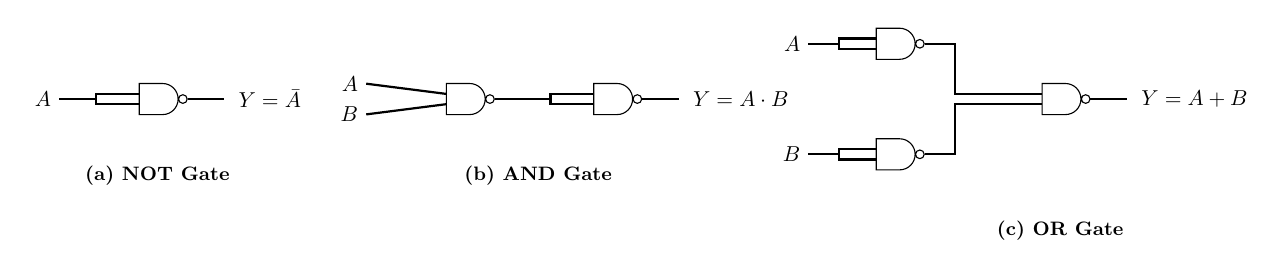
\begin{tikzpicture}[scale=0.78, transform shape]
  % (a) NOT from NAND
  \node[nand gate US, draw, logic gate inputs=nn] (n1) at (1.8, 0) {};
  \draw[thick] (0.2, 0) -- (0.8, 0) node[left, at start] {$A$};
  \draw[thick] (0.8, 0) |- (n1.input 1);
  \draw[thick] (0.8, 0) |- (n1.input 2);
  \draw[thick] (n1.output) -- ++(0.6, 0) node[right, xshift=1mm] {$Y = \bar{A}$};
  \node[below=0.7cm of n1] {\small \textbf{(a) NOT Gate}};

  % (b) AND from NAND
  \node[nand gate US, draw, logic gate inputs=nn] (n2) at (6.8, 0) {};
  \node[nand gate US, draw, logic gate inputs=nn] (n3) at (9.2, 0) {};
  \draw[thick] (5.2, 0.25) -- (n2.input 1) node[left, at start] {$A$};
  \draw[thick] (5.2, -0.25) -- (n2.input 2) node[left, at start] {$B$};
  \draw[thick] (n2.output) -- (8.2, 0);
  \draw[thick] (8.2, 0) |- (n3.input 1);
  \draw[thick] (8.2, 0) |- (n3.input 2);
  \draw[thick] (n3.output) -- ++(0.6, 0) node[right, xshift=1mm] {$Y = A \cdot B$};
  \node[below=0.7cm of n2, xshift=1.2cm] {\small \textbf{(b) AND Gate}};

  % (c) OR from NAND
  \node[nand gate US, draw, logic gate inputs=nn] (n4) at (13.8, 0.9) {};
  \node[nand gate US, draw, logic gate inputs=nn] (n5) at (13.8, -0.9) {};
  \node[nand gate US, draw, logic gate inputs=nn] (n6) at (16.5, 0) {};
  \draw[thick] (12.4, 0.9) -- (12.9, 0.9) node[left, at start] {$A$};
  \draw[thick] (12.9, 0.9) |- (n4.input 1); \draw[thick] (12.9, 0.9) |- (n4.input 2);
  \draw[thick] (12.4, -0.9) -- (12.9, -0.9) node[left, at start] {$B$};
  \draw[thick] (12.9, -0.9) |- (n5.input 1); \draw[thick] (12.9, -0.9) |- (n5.input 2);
  \draw[thick] (n4.output) -- ++(0.5, 0) |- (n6.input 1);
  \draw[thick] (n5.output) -- ++(0.5, 0) |- (n6.input 2);
  \draw[thick] (n6.output) -- ++(0.6, 0) node[right, xshift=1mm] {$Y = A + B$};
  \node[below=1.6cm of n6] {\small \textbf{(c) OR Gate}};
\end{tikzpicture}
\end{schematicbox}

\paragraph{2. Realization of Basic Gates Using NOR Gates Only:}
\begin{itemize}
  \item \textbf{NOT Gate:} Tie both inputs together: $Y = \overline{A + A} = \bar{A}$.
  \item \textbf{OR Gate:} A NOR gate followed by a NOR-inverter: $Y = \overline{\overline{A + B}} = A + B$.
  \item \textbf{AND Gate:} By De Morgan's Law, $A \cdot B = \overline{\bar{A} + \bar{B}}$. Invert $A$ and $B$ with NOR inverters, then apply to a NOR gate: $Y = \overline{\bar{A} + \bar{B}} = A \cdot B$.
\end{itemize}

\begin{schematicbox}{Basic Logic Gates Synthesized from NOR Gates}
\centering
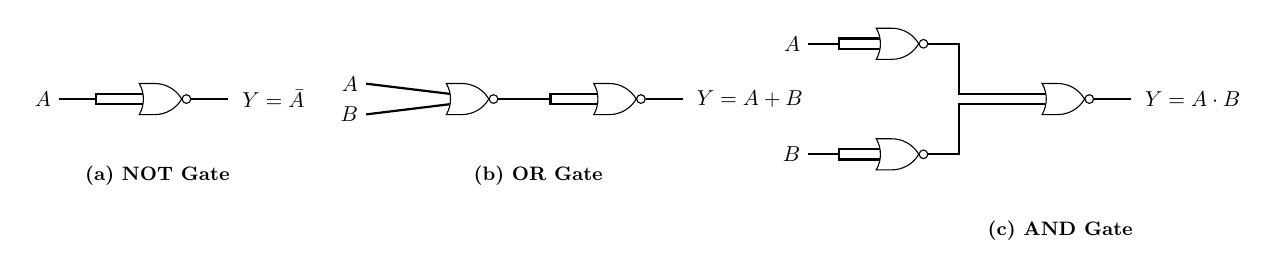
\begin{tikzpicture}[scale=0.78, transform shape]
  % (a) NOT from NOR
  \node[nor gate US, draw, logic gate inputs=nn] (r1) at (1.8, 0) {};
  \draw[thick] (0.2, 0) -- (0.8, 0) node[left, at start] {$A$};
  \draw[thick] (0.8, 0) |- (r1.input 1);
  \draw[thick] (0.8, 0) |- (r1.input 2);
  \draw[thick] (r1.output) -- ++(0.6, 0) node[right, xshift=1mm] {$Y = \bar{A}$};
  \node[below=0.7cm of r1] {\small \textbf{(a) NOT Gate}};

  % (b) OR from NOR
  \node[nor gate US, draw, logic gate inputs=nn] (r2) at (6.8, 0) {};
  \node[nor gate US, draw, logic gate inputs=nn] (r3) at (9.2, 0) {};
  \draw[thick] (5.2, 0.25) -- (r2.input 1) node[left, at start] {$A$};
  \draw[thick] (5.2, -0.25) -- (r2.input 2) node[left, at start] {$B$};
  \draw[thick] (r2.output) -- (8.2, 0);
  \draw[thick] (8.2, 0) |- (r3.input 1);
  \draw[thick] (8.2, 0) |- (r3.input 2);
  \draw[thick] (r3.output) -- ++(0.6, 0) node[right, xshift=1mm] {$Y = A + B$};
  \node[below=0.7cm of r2, xshift=1.2cm] {\small \textbf{(b) OR Gate}};

  % (c) AND from NOR
  \node[nor gate US, draw, logic gate inputs=nn] (r4) at (13.8, 0.9) {};
  \node[nor gate US, draw, logic gate inputs=nn] (r5) at (13.8, -0.9) {};
  \node[nor gate US, draw, logic gate inputs=nn] (r6) at (16.5, 0) {};
  \draw[thick] (12.4, 0.9) -- (12.9, 0.9) node[left, at start] {$A$};
  \draw[thick] (12.9, 0.9) |- (r4.input 1); \draw[thick] (12.9, 0.9) |- (r4.input 2);
  \draw[thick] (12.4, -0.9) -- (12.9, -0.9) node[left, at start] {$B$};
  \draw[thick] (12.9, -0.9) |- (r5.input 1); \draw[thick] (12.9, -0.9) |- (r5.input 2);
  \draw[thick] (r4.output) -- ++(0.5, 0) |- (r6.input 1);
  \draw[thick] (r5.output) -- ++(0.5, 0) |- (r6.input 2);
  \draw[thick] (r6.output) -- ++(0.6, 0) node[right, xshift=1mm] {$Y = A \cdot B$};
  \node[below=1.6cm of r6] {\small \textbf{(c) AND Gate}};
\end{tikzpicture}
\end{schematicbox}

\begin{answerbox}
Since both NAND and NOR gates can independently synthesize the complete set of Boolean operators $\{\text{NOT}, \text{AND}, \text{OR}\}$, they are universally complete logic gates.
\end{answerbox}

\vspace{0.6cm}

% =========================================================================
% QUESTION 4
% =========================================================================
\subsection{Question 4: 4-Variable K-Map Minimization \& Circuit [5 Marks]}
\begin{questionbox}{Problem Statement (2083 Baishakh, Q4)}
Minimize the function $F(A, B, C, D) = \sum m(1, 2, 4, 5, 6, 8, 10, 11, 13, 15)$ using K-Map and realize it with suitable logic gates.
\end{questionbox}

\paragraph{1. Karnaugh Map Plotting (4-Variable K-Map):}
The given minterms are plotted into the $4 \times 4$ Gray-coded map:
\begin{center}
\begin{tabular}{|c|c|c|c|c|}
\hline
$AB \ \backslash \ CD$ & \textbf{00} & \textbf{01} & \textbf{11} & \textbf{10} \\ \hline
\textbf{00} & $0\ (m_0)$ & $\mathbf{1}\ (m_1)$ & $0\ (m_3)$ & $\mathbf{1}\ (m_2)$ \\ \hline
\textbf{01} & $\mathbf{1}\ (m_4)$ & $\mathbf{1}\ (m_5)$ & $0\ (m_7)$ & $\mathbf{1}\ (m_6)$ \\ \hline
\textbf{11} & $0\ (m_{12})$ & $\mathbf{1}\ (m_{13})$ & $\mathbf{1}\ (m_{15})$ & $0\ (m_{14})$ \\ \hline
\textbf{10} & $\mathbf{1}\ (m_8)$ & $0\ (m_9)$ & $\mathbf{1}\ (m_{11})$ & $\mathbf{1}\ (m_{10})$ \\ \hline
\end{tabular}
\end{center}

\paragraph{2. Systematic Grouping (Prime Implicants):}
\begin{enumerate}
  \item \textbf{Group 1 (Quad in column 01):} Minterms $(m_1, m_5, m_{13}, m_{15}) \implies \mathbf{\bar{C}D}$.
  \item \textbf{Group 2 (Pair in row 01):} Minterms $(m_4, m_6) \implies \mathbf{\bar{A}B\bar{D}}$.
  \item \textbf{Group 3 (Pair in column 10):} Minterms $(m_2, m_6) \implies \mathbf{\bar{A}C\bar{D}}$.
  \item \textbf{Group 4 (Pair in row 10):} Minterms $(m_8, m_{10}) \implies \mathbf{A\bar{B}\bar{D}}$.
  \item \textbf{Group 5 (Pair in column 11):} Minterms $(m_{11}, m_{15}) \implies \mathbf{ACD}$.
  \item \textbf{Group 6 (Pair in row 11):} Minterms $(m_{13}, m_{15}) \implies \mathbf{ABD}$.
\end{enumerate}
The minimal Sum of Products (SOP) expression is:
\[
F(A,B,C,D) = \bar{A}\bar{C}D + \bar{A}B\bar{D} + \bar{A}C\bar{D} + A\bar{B}\bar{D} + ACD + ABD
\]

\begin{schematicbox}{Two-Level AND-OR Logic Realization for Minimized $F(A,B,C,D)$}
\centering
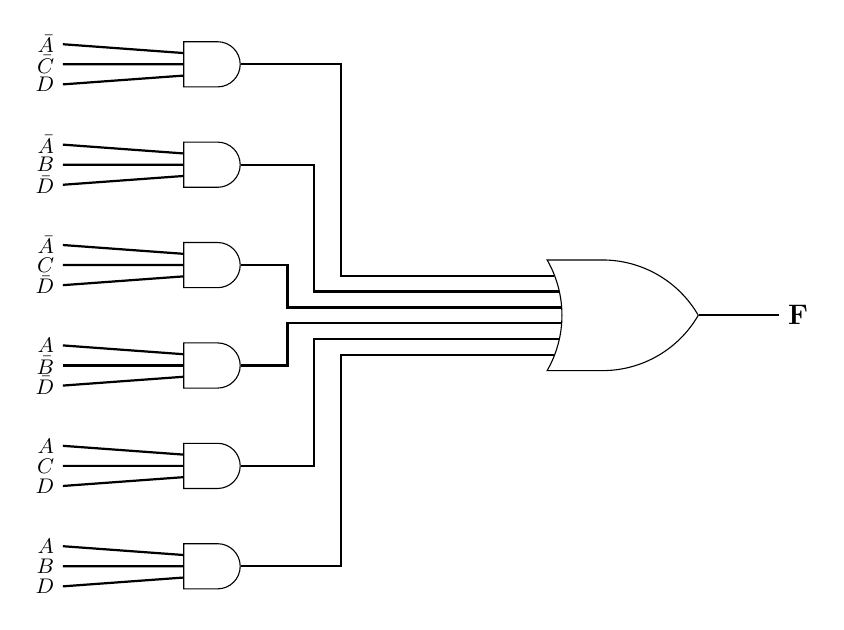
\begin{tikzpicture}[scale=0.85, transform shape]
  % 6 AND Gates
  \foreach \i/\label/\inA/\inB/\inC in {
    1/{$\bar{A}\bar{C}D$}/$\bar{A}$/$\bar{C}$/$D$,
    2/{$\bar{A}B\bar{D}$}/$\bar{A}$/$B$/$\bar{D}$,
    3/{$\bar{A}C\bar{D}$}/$\bar{A}$/$C$/$\bar{D}$,
    4/{\smash{$A\bar{B}\bar{D}$}}/$A$/$\bar{B}$/$\bar{D}$,
    5/{$ACD$}/$A$/$C$/$D$,
    6/{$ABD$}/$A$/$B$/$D$
  } {
    \node[and gate US, draw, logic gate inputs=nnn] (and\i) at (4, {4.5 - (\i - 1)*1.5}) {};
    \draw[thick] (1.8, {4.5 - (\i - 1)*1.5 + 0.3}) node[left] {\small \inA} -- (and\i.input 1);
    \draw[thick] (1.8, {4.5 - (\i - 1)*1.5}) node[left] {\small \inB} -- (and\i.input 2);
    \draw[thick] (1.8, {4.5 - (\i - 1)*1.5 - 0.3}) node[left] {\small \inC} -- (and\i.input 3);
  }

  % 6-input OR Gate
  \node[or gate US, draw, logic gate inputs=nnnnnn, scale=1.4] (orgate) at (10, 0.75) {};
  
  \draw[thick] (and1.output) -- ++(1.5, 0) |- (orgate.input 1);
  \draw[thick] (and2.output) -- ++(1.1, 0) |- (orgate.input 2);
  \draw[thick] (and3.output) -- ++(0.7, 0) |- (orgate.input 3);
  \draw[thick] (and4.output) -- ++(0.7, 0) |- (orgate.input 4);
  \draw[thick] (and5.output) -- ++(1.1, 0) |- (orgate.input 5);
  \draw[thick] (and6.output) -- ++(1.5, 0) |- (orgate.input 6);
  
  \draw[thick] (orgate.output) -- ++(1.2, 0) node[right] {\large $\mathbf{F}$};
\end{tikzpicture}
\end{schematicbox}

\begin{answerbox}
$$\mathbf{F(A,B,C,D) = \bar{A}\bar{C}D + \bar{A}B\bar{D} + \bar{A}C\bar{D} + A\bar{B}\bar{D} + ACD + ABD}$$
\end{answerbox}

\vspace{0.6cm}

% =========================================================================
% QUESTION 5
% =========================================================================
\subsection{Question 5: Octal-to-Binary Encoder Logic Circuit [2 + 4 = 6 Marks]}
\begin{questionbox}{Problem Statement (2083 Baishakh, Q5)}
Differentiate between encoder and decoder. Design an octal-to-binary encoder with necessary diagrams.
\end{questionbox}

\paragraph{Part (a): Comparison between Encoder and Decoder [2 Marks]}
\begin{center}
\small
\begin{tabular}{@{}p{3.2cm}p{6.8cm}p{6.8cm}@{}}
\toprule
\textbf{Feature} & \textbf{Encoder} & \textbf{Decoder} \\
\midrule
\textbf{Functional Operation} & Converts $2^n$ (or fewer) input active lines into an $n$-bit coded binary output. & Converts an $n$-bit coded binary input into $2^n$ unique active output lines. \\
\textbf{Inputs / Outputs} & $2^n$ input lines, $n$ output lines. & $n$ input lines, $2^n$ output lines. \\
\textbf{Internal Logic Gate} & Constructed using \textbf{OR} gates. & Constructed using \textbf{AND} / \textbf{NAND} gates. \\
\textbf{Typical Applications} & Keyboards, priority encoders, Flash Analog-to-Digital Converters (ADCs). & Memory address decoding, 7-segment display drivers, demultiplexers. \\
\bottomrule
\end{tabular}
\end{center}

\paragraph{Part (b): Design of Octal-to-Binary Encoder (8-to-3 Encoder) [4 Marks]}
An octal-to-binary encoder accepts 8 active-high input lines $D_0, D_1, \dots, D_7$ (where exactly one input is HIGH at any instant) and produces a 3-bit binary equivalent $A, B, C$ ($A$ is MSB, $C$ is LSB).

\paragraph{Truth Table:}
\begin{center}
\begin{tabular}{|cccccccc||ccc|}
\hline
$D_7$ & $D_6$ & $D_5$ & $D_4$ & $D_3$ & $D_2$ & $D_1$ & $D_0$ & $\mathbf{A\ (MSB)}$ & $\mathbf{B}$ & $\mathbf{C\ (LSB)}$ \\ \hline
0 & 0 & 0 & 0 & 0 & 0 & 0 & 1 & 0 & 0 & 0 \\ \hline
0 & 0 & 0 & 0 & 0 & 0 & 1 & 0 & 0 & 0 & 1 \\ \hline
0 & 0 & 0 & 0 & 0 & 1 & 0 & 0 & 0 & 1 & 0 \\ \hline
0 & 0 & 0 & 0 & 1 & 0 & 0 & 0 & 0 & 1 & 1 \\ \hline
0 & 0 & 0 & 1 & 0 & 0 & 0 & 0 & 1 & 0 & 0 \\ \hline
0 & 0 & 1 & 0 & 0 & 0 & 0 & 0 & 1 & 0 & 1 \\ \hline
0 & 1 & 0 & 0 & 0 & 0 & 0 & 0 & 1 & 1 & 0 \\ \hline
1 & 0 & 0 & 0 & 0 & 0 & 0 & 0 & 1 & 1 & 1 \\ \hline
\end{tabular}
\end{center}

\paragraph{Boolean Output Equations:}
Output bits are HIGH whenever any input corresponding to that binary position is active:
\begin{align*}
A &= D_4 + D_5 + D_6 + D_7 \\
B &= D_2 + D_3 + D_6 + D_7 \\
C &= D_1 + D_3 + D_5 + D_7
\end{align*}
(Note: $D_0$ is not required in the equations since $A=B=C=0$ when $D_0=1$.)

\begin{schematicbox}{Octal-to-Binary (8-to-3) Encoder Logic Schematic}
\centering
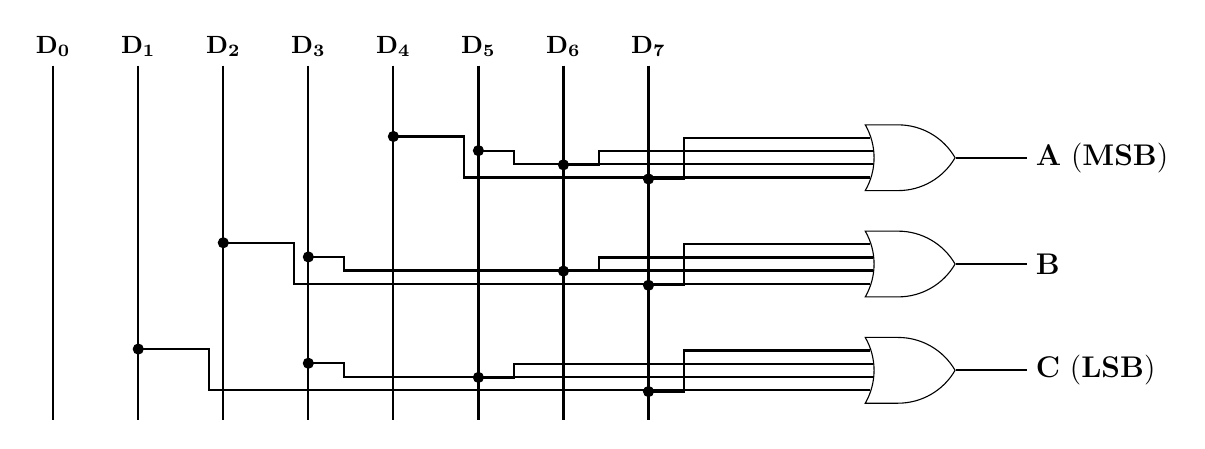
\begin{tikzpicture}[scale=0.9, transform shape]
  % Vertical input lines D0 to D7
  \foreach \i in {0,1,...,7} {
    \draw[thick] ({1.2*\i}, 5.5) -- ({1.2*\i}, 0.5);
    \node[above] at ({1.2*\i}, 5.5) {$\mathbf{D_\i}$};
  }

  % Horizontal OR gates on the right
  \node[or gate US, draw, logic gate inputs=nnnn, scale=1.1] (orA) at (12.0, 4.2) {};
  \node[or gate US, draw, logic gate inputs=nnnn, scale=1.1] (orB) at (12.0, 2.7) {};
  \node[or gate US, draw, logic gate inputs=nnnn, scale=1.1] (orC) at (12.0, 1.2) {};

  % Output lines
  \draw[thick] (orA.output) -- ++(1.0, 0) node[right] {\large $\mathbf{A\ (MSB)}$};
  \draw[thick] (orB.output) -- ++(1.0, 0) node[right] {\large $\mathbf{B}$};
  \draw[thick] (orC.output) -- ++(1.0, 0) node[right] {\large $\mathbf{C\ (LSB)}$};

  % Wiring for OR A: D4, D5, D6, D7
  \filldraw[black] ({1.2*4}, 4.5) circle (2pt); \draw[thick] ({1.2*4}, 4.5) -- ++(1.0, 0) |- (orA.input 4);
  \filldraw[black] ({1.2*5}, 4.3) circle (2pt); \draw[thick] ({1.2*5}, 4.3) -- ++(0.5, 0) |- (orA.input 3);
  \filldraw[black] ({1.2*6}, 4.1) circle (2pt); \draw[thick] ({1.2*6}, 4.1) -- ++(0.5, 0) |- (orA.input 2);
  \filldraw[black] ({1.2*7}, 3.9) circle (2pt); \draw[thick] ({1.2*7}, 3.9) -- ++(0.5, 0) |- (orA.input 1);

  % Wiring for OR B: D2, D3, D6, D7
  \filldraw[black] ({1.2*2}, 3.0) circle (2pt); \draw[thick] ({1.2*2}, 3.0) -- ++(1.0, 0) |- (orB.input 4);
  \filldraw[black] ({1.2*3}, 2.8) circle (2pt); \draw[thick] ({1.2*3}, 2.8) -- ++(0.5, 0) |- (orB.input 3);
  \filldraw[black] ({1.2*6}, 2.6) circle (2pt); \draw[thick] ({1.2*6}, 2.6) -- ++(0.5, 0) |- (orB.input 2);
  \filldraw[black] ({1.2*7}, 2.4) circle (2pt); \draw[thick] ({1.2*7}, 2.4) -- ++(0.5, 0) |- (orB.input 1);

  % Wiring for OR C: D1, D3, D5, D7
  \filldraw[black] ({1.2*1}, 1.5) circle (2pt); \draw[thick] ({1.2*1}, 1.5) -- ++(1.0, 0) |- (orC.input 4);
  \filldraw[black] ({1.2*3}, 1.3) circle (2pt); \draw[thick] ({1.2*3}, 1.3) -- ++(0.5, 0) |- (orC.input 3);
  \filldraw[black] ({1.2*5}, 1.1) circle (2pt); \draw[thick] ({1.2*5}, 1.1) -- ++(0.5, 0) |- (orC.input 2);
  \filldraw[black] ({1.2*7}, 0.9) circle (2pt); \draw[thick] ({1.2*7}, 0.9) -- ++(0.5, 0) |- (orC.input 1);
\end{tikzpicture}
\end{schematicbox}

\begin{answerbox}
$$\mathbf{A = D_4 + D_5 + D_6 + D_7, \quad B = D_2 + D_3 + D_6 + D_7, \quad C = D_1 + D_3 + D_5 + D_7}$$
\end{answerbox}

\vspace{0.6cm}

% =========================================================================
% QUESTION 6
% =========================================================================
\subsection{Question 6: Full Subtractor Using Multiplexers [4 Marks]}
\begin{questionbox}{Problem Statement (2083 Baishakh, Q6)}
Implement a full subtractor circuit using multiplexer.
\end{questionbox}

A full subtractor performs subtraction on three 1-bit inputs: Minuend ($A$), Subtrahend ($B$), and Borrow In ($B_{\text{in}}$). It generates Difference ($D$) and Borrow Out ($B_{\text{out}}$).

\paragraph{Truth Table:}
\begin{center}
\begin{tabular}{|ccc||cc|}
\hline
$A$ & $B$ & $B_{\text{in}}$ & $\mathbf{D\ (Difference)}$ & $\mathbf{B_{\text{out}}\ (Borrow)}$ \\ \hline
0 & 0 & 0 & 0 & 0 \\ \hline
0 & 0 & 1 & 1 & 1 \\ \hline
0 & 1 & 0 & 1 & 1 \\ \hline
0 & 1 & 1 & 0 & 1 \\ \hline
1 & 0 & 0 & 1 & 0 \\ \hline
1 & 0 & 1 & 0 & 0 \\ \hline
1 & 1 & 0 & 0 & 0 \\ \hline
1 & 1 & 1 & 1 & 1 \\ \hline
\end{tabular}
\end{center}
Minterm canonical forms:
\[
D(A,B,B_{\text{in}}) = \sum m(1, 2, 4, 7), \qquad B_{\text{out}}(A,B,B_{\text{in}}) = \sum m(1, 2, 3, 7)
\]

\paragraph{Multiplexer Implementation using Two $4:1$ MUXes:}
Let select lines be $S_1 = A$ and $S_0 = B$, and data inputs be expressed in terms of $B_{\text{in}}$:
\begin{center}
\begin{tabular}{|c|c|c|c|}
\hline
\textbf{Select Inputs} $(A, B)$ & \textbf{Data Channel} & \textbf{Difference ($D$)} & \textbf{Borrow Out ($B_{\text{out}}$)} \\ \hline
$00$ & $I_0$ & $B_{\text{in}}$ & $B_{\text{in}}$ \\ \hline
$01$ & $I_1$ & $\bar{B}_{\text{in}}$ & $1\ (V_{CC})$ \\ \hline
$10$ & $I_2$ & $\bar{B}_{\text{in}}$ & $0\ (\text{GND})$ \\ \hline
$11$ & $I_3$ & $B_{\text{in}}$ & $B_{\text{in}}$ \\ \hline
\end{tabular}
\end{center}

\begin{schematicbox}{Full Subtractor Implementation Using Two 4:1 Multiplexers}
\centering
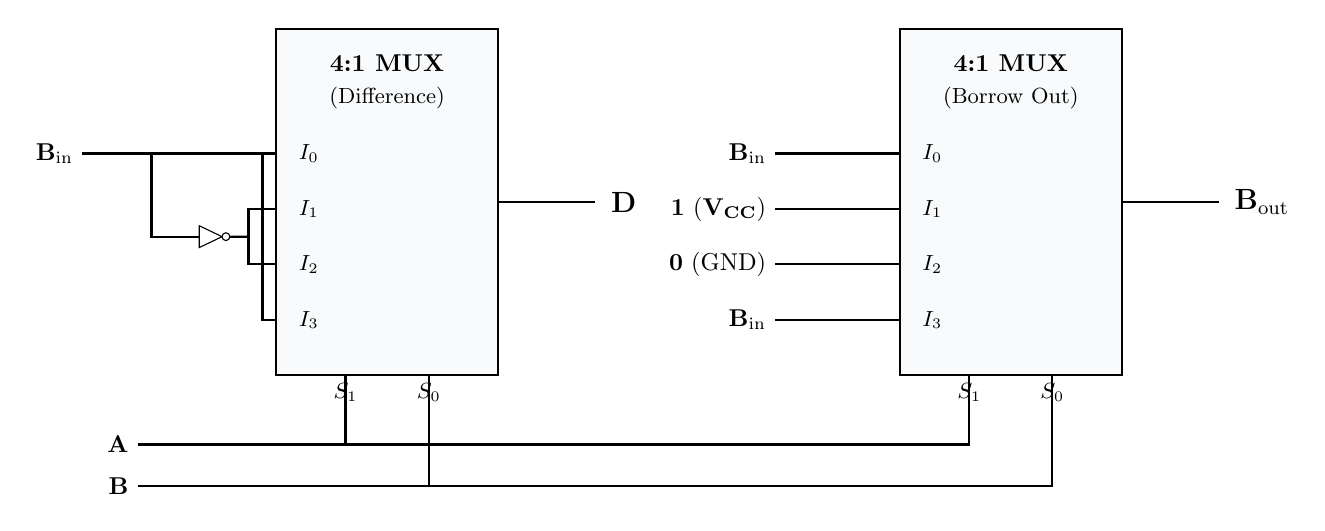
\begin{tikzpicture}[scale=0.88, transform shape]
  % MUX 1: Difference (x: 0 to 3.2)
  \draw[thick, fill=boxbg] (0, 0) rectangle (3.2, 5.0);
  \node at (1.6, 4.5) {\textbf{4:1 MUX}};
  \node at (1.6, 4.0) {\small (Difference)};
  \node[anchor=west] at (0.2, 3.2) {\small $I_0$};
  \node[anchor=west] at (0.2, 2.4) {\small $I_1$};
  \node[anchor=west] at (0.2, 1.6) {\small $I_2$};
  \node[anchor=west] at (0.2, 0.8) {\small $I_3$};
  \node[anchor=north] at (1.0, 0) {\small $S_1$};
  \node[anchor=north] at (2.2, 0) {\small $S_0$};
  \draw[thick] (3.2, 2.5) -- ++(1.4, 0) node[right, xshift=1mm] {\large $\mathbf{D}$};

  % MUX 2: Borrow Out (x: 9.0 to 12.2)
  \draw[thick, fill=boxbg] (9.0, 0) rectangle (12.2, 5.0);
  \node at (10.6, 4.5) {\textbf{4:1 MUX}};
  \node at (10.6, 4.0) {\small (Borrow Out)};
  \node[anchor=west] at (9.2, 3.2) {\small $I_0$};
  \node[anchor=west] at (9.2, 2.4) {\small $I_1$};
  \node[anchor=west] at (9.2, 1.6) {\small $I_2$};
  \node[anchor=west] at (9.2, 0.8) {\small $I_3$};
  \node[anchor=north] at (10.0, 0) {\small $S_1$};
  \node[anchor=north] at (11.2, 0) {\small $S_0$};
  \draw[thick] (12.2, 2.5) -- ++(1.4, 0) node[right, xshift=1mm] {\large $\mathbf{B_{\text{out}}}$};

  % Input Rails on Left for MUX 1
  \draw[thick] (-2.8, 3.2) node[left] {$\mathbf{B_{\text{in}}}$} -- (-1.8, 3.2);
  \node[not gate US, draw, scale=0.8] (not1) at (-1.0, 2.0) {};
  \draw[thick] (-1.8, 3.2) -- (-0.2, 3.2) -- (0, 3.2);
  \draw[thick] (-1.8, 3.2) |- (not1.input);
  \draw[thick] (not1.output) -- (-0.4, 2.0);
  \draw[thick] (-0.4, 2.0) |- (0, 2.4);
  \draw[thick] (-0.4, 2.0) |- (0, 1.6);
  \draw[thick] (-0.2, 3.2) |- (0, 0.8);

  % Inputs for MUX 2
  \draw[thick] (7.2, 3.2) node[left] {$\mathbf{B_{\text{in}}}$} -- (9.0, 3.2);
  \draw[thick] (7.2, 2.4) node[left] {$\mathbf{1\ (V_{CC})}$} -- (9.0, 2.4);
  \draw[thick] (7.2, 1.6) node[left] {$\mathbf{0\ (\text{GND})}$} -- (9.0, 1.6);
  \draw[thick] (7.2, 0.8) node[left] {$\mathbf{B_{\text{in}}}$} -- (9.0, 0.8);

  % Common Select lines A, B
  \draw[thick] (-2.0, -1.0) node[left] {$\mathbf{A}$} -- (1.0, -1.0) -- (1.0, 0);
  \draw[thick] (1.0, -1.0) -- (10.0, -1.0) -- (10.0, 0);
  \draw[thick] (-2.0, -1.6) node[left] {$\mathbf{B}$} -- (2.2, -1.6) -- (2.2, 0);
  \draw[thick] (2.2, -1.6) -- (11.2, -1.6) -- (11.2, 0);
\end{tikzpicture}
\end{schematicbox}

\begin{answerbox}
\textbf{Difference ($D$):} $I_0 = B_{\text{in}}, I_1 = \bar{B}_{\text{in}}, I_2 = \bar{B}_{\text{in}}, I_3 = B_{\text{in}}$.\\
\textbf{Borrow Out ($B_{\text{out}}$):} $I_0 = B_{\text{in}}, I_1 = 1, I_2 = 0, I_3 = B_{\text{in}}$, with select lines $S_1 = A, S_0 = B$.
\end{answerbox}

\vspace{0.6cm}

% =========================================================================
% QUESTION 7
% =========================================================================
\subsection{Question 7: D Flip-Flop to JK Flip-Flop Conversion Schematic [2 + 5 = 7 Marks]}
\begin{questionbox}{Problem Statement (2083 Baishakh, Q7)}
Differentiate between latch and flipflop. Modify a D flip-flop such that it functions as a JK flip-flop.
\end{questionbox}

\paragraph{Part (a): Comparison between Latch and Flip-Flop [2 Marks]}
\begin{center}
\small
\begin{tabular}{@{}p{3.2cm}p{6.8cm}p{6.8cm}@{}}
\toprule
\textbf{Parameter} & \textbf{Latch} & \textbf{Flip-Flop} \\
\midrule
\textbf{Triggering Method} & \textbf{Level-triggered}: transparent to input changes as long as Enable (EN) is active HIGH/LOW. & \textbf{Edge-triggered}: state transition occurs only during an active clock transition ($\uparrow$ positive or $\downarrow$ negative edge). \\
\textbf{Clock Requirement} & Does not require a periodic clock signal; operates on control/enable gates. & Requires a synchronous periodic clock signal for synchronized state updates. \\
\textbf{Race Condition} & Highly susceptible to race-around conditions when pulse width exceeds propagation delay. & Immune to race-around condition because input sampling occurs only during infinitesimal clock edges. \\
\textbf{Circuit Role} & Asynchronous registers, temporary storage buffers. & Synchronous counters, state machines, pipelines, CPU registers. \\
\bottomrule
\end{tabular}
\end{center}

\paragraph{Part (b): Conversion of D Flip-Flop to JK Flip-Flop [5 Marks]}
\begin{enumerate}
  \item \textbf{Target Behavior:} JK Flip-Flop with inputs $J, K$, present state $Q_n$, and next state $Q_{n+1}$.
  \item \textbf{Available Device:} D Flip-Flop whose characteristic equation is $Q_{n+1} = D$. Thus, $D = Q_{n+1}$.
\end{enumerate}

\paragraph{Conversion Table:}
\begin{center}
\begin{tabular}{|ccc||c||c|}
\hline
$\mathbf{J}$ & $\mathbf{K}$ & $\mathbf{Q_n}$ & $\mathbf{Q_{n+1}}$ & $\mathbf{D\ \text{Input}\ (D = Q_{n+1})}$ \\ \hline
0 & 0 & 0 & 0 & 0 \\ \hline
0 & 0 & 1 & 1 & 1 \\ \hline
0 & 1 & 0 & 0 & 0 \\ \hline
0 & 1 & 1 & 0 & 0 \\ \hline
1 & 0 & 0 & 1 & 1 \\ \hline
1 & 0 & 1 & 1 & 1 \\ \hline
1 & 1 & 0 & 1 & 1 \\ \hline
1 & 1 & 1 & 0 & 0 \\ \hline
\end{tabular}
\end{center}

\paragraph{K-Map for Input $D(J, K, Q_n)$:}
\begin{center}
\begin{tabular}{|c|c|c|}
\hline
$JK \ \backslash \ Q_n$ & $\mathbf{0}$ & $\mathbf{1}$ \\ \hline
\textbf{00} & $0$ & $1$ \\ \hline
\textbf{01} & $0$ & $0$ \\ \hline
\textbf{11} & $1$ & $0$ \\ \hline
\textbf{10} & $1$ & $1$ \\ \hline
\end{tabular}
\end{center}
\begin{itemize}
  \item Group 1: Minterms for $Q_n=0$ where $J=1 \implies \mathbf{J\bar{Q}_n}$
  \item Group 2: Minterms for $Q_n=1$ where $K=0 \implies \mathbf{\bar{K}Q_n}$
\end{itemize}
\[
D = J\bar{Q} + \bar{K}Q
\]

\begin{schematicbox}{JK Flip-Flop Realized by Modifying a D Flip-Flop}
\centering
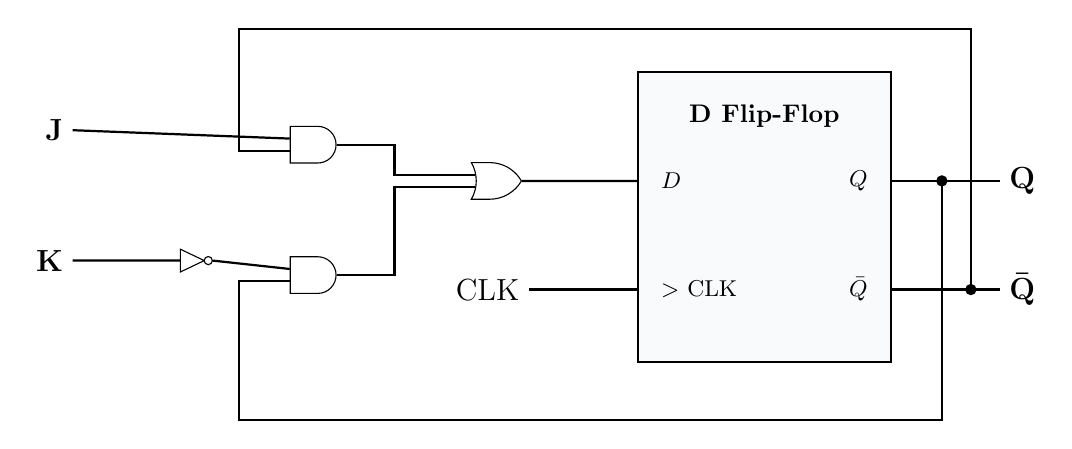
\begin{tikzpicture}[scale=0.92, transform shape]
  % D Flip Flop Box
  \draw[thick, fill=boxbg] (7.0, 0) rectangle (10.5, 4.0);
  \node at (8.75, 3.4) {\textbf{D Flip-Flop}};
  \node[anchor=west] at (7.2, 2.5) {\small $D$};
  \node[anchor=west] at (7.2, 1.0) {\small $>$ \text{CLK}};
  \node[anchor=east] at (10.3, 2.5) {\small $Q$};
  \node[anchor=east] at (10.3, 1.0) {\small $\bar{Q}$};

  % Clock line
  \draw[thick] (5.5, 1.0) -- (7.0, 1.0) node[left, at start] {\large $\mathbf{\text{CLK}}$};

  % Logic gates on the left
  \node[and gate US, draw, logic gate inputs=nn] (and1) at (2.5, 3.0) {};
  \node[and gate US, draw, logic gate inputs=nn] (and2) at (2.5, 1.2) {};
  \node[not gate US, draw, scale=0.8] (notK) at (0.8, 1.4) {};
  \node[or gate US, draw, logic gate inputs=nn] (orgate) at (5.0, 2.5) {};

  % Inputs J and K
  \draw[thick] (-0.8, 3.2) -- (and1.input 1) node[left, at start] {\large $\mathbf{J}$};
  \draw[thick] (-0.8, 1.4) -- (notK.input) node[left, at start] {\large $\mathbf{K}$};
  \draw[thick] (notK.output) -- (and2.input 1);

  % OR gate to D input
  \draw[thick] (and1.output) -- ++(0.8, 0) |- (orgate.input 1);
  \draw[thick] (and2.output) -- ++(0.8, 0) |- (orgate.input 2);
  \draw[thick] (orgate.output) -- (7.0, 2.5);

  % Feedback paths Q and Q_bar
  \draw[thick] (10.5, 2.5) -- ++(1.5, 0) node[right] {\large $\mathbf{Q}$};
  \draw[thick] (10.5, 1.0) -- ++(1.5, 0) node[right] {\large $\mathbf{\bar{Q}}$};

  % Feedback Q to and2.input 2
  \filldraw[black] (11.2, 2.5) circle (2pt);
  \draw[thick] (11.2, 2.5) -- (11.2, -0.8) -- (1.5, -0.8) |- (and2.input 2);

  % Feedback Q_bar to and1.input 2
  \filldraw[black] (11.6, 1.0) circle (2pt);
  \draw[thick] (11.6, 1.0) -- (11.6, 4.6) -- (1.5, 4.6) |- (and1.input 2);
\end{tikzpicture}
\end{schematicbox}

\begin{answerbox}
$$\mathbf{D = J\bar{Q} + \bar{K}Q}$$
A D flip-flop is transformed into a JK flip-flop by driving its $D$ input with the combinational network $J\bar{Q} + \bar{K}Q$.
\end{answerbox}

\vspace{0.6cm}

% =========================================================================
% QUESTION 8
% =========================================================================
\subsection{Question 8: 4-Bit SIPO Shift Register Schematic \& Timing Diagram [5 Marks]}
\begin{questionbox}{Problem Statement (2083 Baishakh, Q8)}
Explain the working of 4-bit SIPO register with timing diagram of 1010 data input.
\end{questionbox}

A \textbf{Serial-In Parallel-Out (SIPO)} shift register accepts binary data sequentially (bit-by-bit) over a single input line, shifting it through cascaded flip-flops on each clock edge. After 4 clock cycles, all 4 bits are simultaneously accessible on parallel output pins $Q_3, Q_2, Q_1, Q_0$.

\begin{schematicbox}{4-Bit Serial-In Parallel-Out (SIPO) Shift Register}
\centering
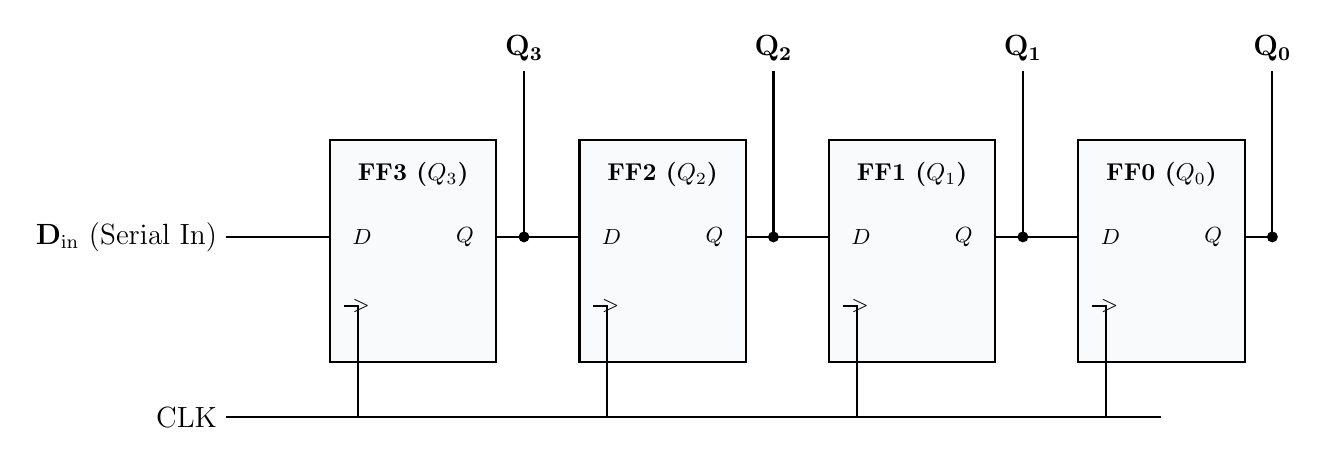
\begin{tikzpicture}[scale=0.88, transform shape]
  % 4 D Flip-Flops
  \foreach \i/\ffname in {3/FF3 ($Q_3$), 2/FF2 ($Q_2$), 1/FF1 ($Q_1$), 0/FF0 ($Q_0$)} {
    \draw[thick, fill=boxbg] ({3.6*(3 - \i)}, 0) rectangle ({3.6*(3 - \i) + 2.4}, 3.2);
    \node at ({3.6*(3 - \i) + 1.2}, 2.7) {\textbf{\ffname}};
    \node[anchor=west] at ({3.6*(3 - \i) + 0.2}, 1.8) {\small $D$};
    \node[anchor=west] at ({3.6*(3 - \i) + 0.2}, 0.8) {\small $>$};
    \node[anchor=east] at ({3.6*(3 - \i) + 2.2}, 1.8) {\small $Q$};
    
    % Parallel output taps
    \filldraw[black] ({3.6*(3 - \i) + 2.8}, 1.8) circle (2pt);
    \draw[thick] ({3.6*(3 - \i) + 2.8}, 1.8) -- ({3.6*(3 - \i) + 2.8}, 4.2) node[above] {\large $\mathbf{Q_\i}$};
  }

  % Serial Input to FF3
  \draw[thick] (-1.5, 1.8) node[left] {\large $\mathbf{D_{\text{in}}\ (\text{Serial In})}$} -- (0, 1.8);

  % Inter-stage connections
  \draw[thick] (2.4, 1.8) -- (3.6, 1.8);
  \draw[thick] (6.0, 1.8) -- (7.2, 1.8);
  \draw[thick] (9.6, 1.8) -- (10.8, 1.8);
  \draw[thick] (13.2, 1.8) -- (13.6, 1.8);

  % Common Clock Rail
  \draw[thick] (-1.5, -0.8) node[left] {\large $\mathbf{\text{CLK}}$} -- (12.0, -0.8);
  \foreach \i in {0,1,2,3} {
    \draw[thick] ({3.6*\i + 0.4}, -0.8) -- ({3.6*\i + 0.4}, 0.8) -- ({3.6*\i + 0.2}, 0.8);
  }
\end{tikzpicture}
\end{schematicbox}

\paragraph{Step-by-Step Operation for Input Sequence $1010_2$ (MSB entered first):}
Assume initial contents are $Q_3 Q_2 Q_1 Q_0 = 0000_2$.
\begin{center}
\begin{tabular}{|c|c|cccc|l|}
\hline
\textbf{Clock Pulse} & \textbf{Serial Input ($D_{\text{in}}$)} & $\mathbf{Q_3}$ & $\mathbf{Q_2}$ & $\mathbf{Q_1}$ & $\mathbf{Q_0}$ & \textbf{Remarks} \\ \hline
\textbf{Initial} & $-$ & 0 & 0 & 0 & 0 & Cleared state \\ \hline
\textbf{CLK 1} & $1$ (MSB) & 1 & 0 & 0 & 0 & First bit enters FF3 \\ \hline
\textbf{CLK 2} & $0$ & 0 & 1 & 0 & 0 & Shift right, second bit enters \\ \hline
\textbf{CLK 3} & $1$ & 1 & 0 & 1 & 0 & Shift right, third bit enters \\ \hline
\textbf{CLK 4} & $0$ (LSB) & 0 & 1 & 0 & 1 & Complete word loaded ($1010_2$) \\ \hline
\end{tabular}
\end{center}

\begin{schematicbox}{Timing Waveforms for 4-Bit SIPO Shift Register Loading $1010_2$}
\centering
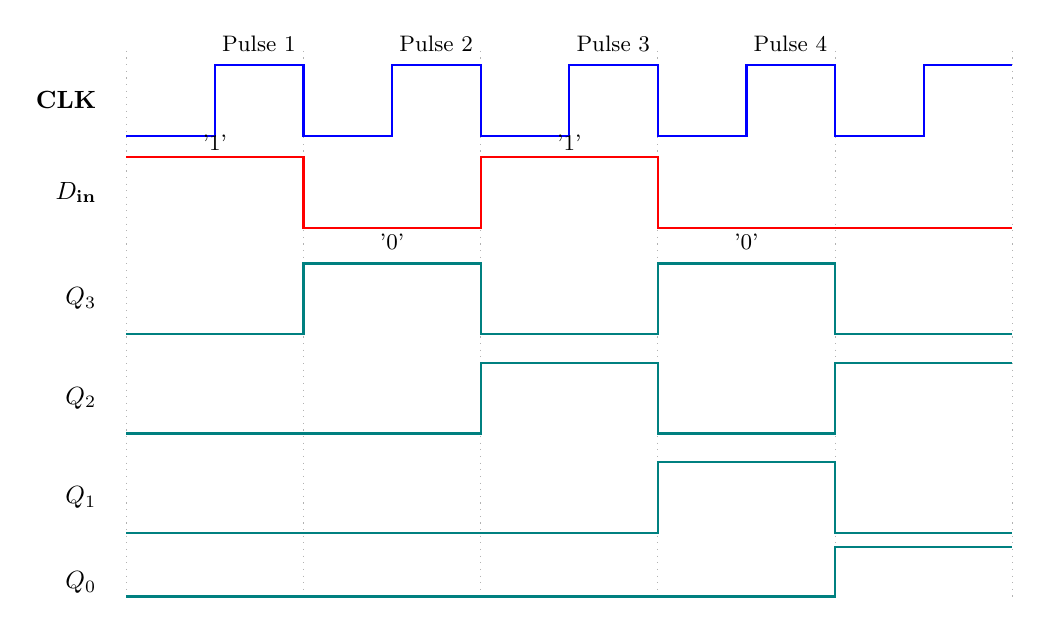
\begin{tikzpicture}[scale=0.9, transform shape]
  % Vertical grid lines
  \foreach \x in {0, 2.5, 5.0, 7.5, 10.0, 12.5} {
    \draw[dotted, gray!60] (\x, 1.2) -- (\x, -6.5);
  }
  
  % Clock Waveform
  \node[left] at (-0.3, 0.5) {\textbf{CLK}};
  \draw[thick, blue] (0,0) -- (1.25,0) -- (1.25,1) -- (2.5,1) -- (2.5,0) -- (3.75,0) -- (3.75,1) -- (5.0,1) -- (5.0,0) -- (6.25,0) -- (6.25,1) -- (7.5,1) -- (7.5,0) -- (8.75,0) -- (8.75,1) -- (10.0,1) -- (10.0,0) -- (11.25,0) -- (11.25,1) -- (12.5,1);
  \node at (1.87, 1.3) {\small Pulse 1};
  \node at (4.37, 1.3) {\small Pulse 2};
  \node at (6.87, 1.3) {\small Pulse 3};
  \node at (9.37, 1.3) {\small Pulse 4};

  % Serial In (1, 0, 1, 0)
  \node[left] at (-0.3, -0.8) {\textbf{$D_{\text{in}}$}};
  \draw[thick, red] (0, -0.3) -- (2.5, -0.3) -- (2.5, -1.3) -- (5.0, -1.3) -- (5.0, -0.3) -- (7.5, -0.3) -- (7.5, -1.3) -- (12.5, -1.3);
  \node at (1.25, -0.1) {\small '1'}; \node at (3.75, -1.5) {\small '0'}; \node at (6.25, -0.1) {\small '1'}; \node at (8.75, -1.5) {\small '0'};

  % Q3
  \node[left] at (-0.3, -2.3) {\textbf{$Q_3$}};
  \draw[thick, teal] (0, -2.8) -- (2.5, -2.8) -- (2.5, -1.8) -- (5.0, -1.8) -- (5.0, -2.8) -- (7.5, -2.8) -- (7.5, -1.8) -- (10.0, -1.8) -- (10.0, -2.8) -- (12.5, -2.8);

  % Q2
  \node[left] at (-0.3, -3.7) {\textbf{$Q_2$}};
  \draw[thick, teal] (0, -4.2) -- (5.0, -4.2) -- (5.0, -3.2) -- (7.5, -3.2) -- (7.5, -4.2) -- (10.0, -4.2) -- (10.0, -3.2) -- (12.5, -3.2);

  % Q1
  \node[left] at (-0.3, -5.1) {\textbf{$Q_1$}};
  \draw[thick, teal] (0, -5.6) -- (7.5, -5.6) -- (7.5, -4.6) -- (10.0, -4.6) -- (10.0, -5.6) -- (12.5, -5.6);

  % Q0
  \node[left] at (-0.3, -6.3) {\textbf{$Q_0$}};
  \draw[thick, teal] (0, -6.5) -- (10.0, -6.5) -- (10.0, -5.8) -- (12.5, -5.8);
\end{tikzpicture}
\end{schematicbox}

\begin{answerbox}
After 4 clock pulses, serial word $1010_2$ is converted to parallel outputs: $\mathbf{Q_3 Q_2 Q_1 Q_0 = 0101_2}$ (or $1010_2$ when read in arrival sequence $Q_0 Q_1 Q_2 Q_3$).
\end{answerbox}

\vspace{0.6cm}

% =========================================================================
% QUESTION 9
% =========================================================================
\subsection{Question 9: Asynchronous BCD (Decade) Counter Schematic [5 Marks]}
\begin{questionbox}{Problem Statement (2083 Baishakh, Q9)}
Describe the operation of asynchronous BCD (decade) counter with necessary diagrams.
\end{questionbox}

An \textbf{Asynchronous BCD (Decade) Counter} (Mod-10 ripple counter) counts through $10$ discrete binary states from $0000_2$ ($0_{10}$) up to $1001_2$ ($9_{10}$) and automatically recycles to $0000_2$ on the tenth clock pulse.

\paragraph{Design Principle:}
\begin{itemize}
  \item 4 negative edge-triggered JK (or T) flip-flops are connected in toggle mode ($J=K=1$).
  \item Ripple clocking: $Q_0 \to \text{CLK}_1$, $Q_1 \to \text{CLK}_2$, $Q_2 \to \text{CLK}_3$.
  \item Modulo reset: At the 10th clock pulse, the count momentarily enters transient state $1010_2$ ($Q_3=1, Q_2=0, Q_1=1, Q_0=0$).
  \item A 2-input NAND gate detects $Q_3 \cdot Q_1 = 1$ and outputs an active-LOW reset pulse ($\overline{\text{CLR}} = 0$) to all flip-flops:
  \[
  \overline{\text{CLR}} = \overline{Q_3 \cdot Q_1}
  \]
\end{itemize}

\begin{schematicbox}{Asynchronous BCD (Decade) Counter Logic Circuit}
\centering
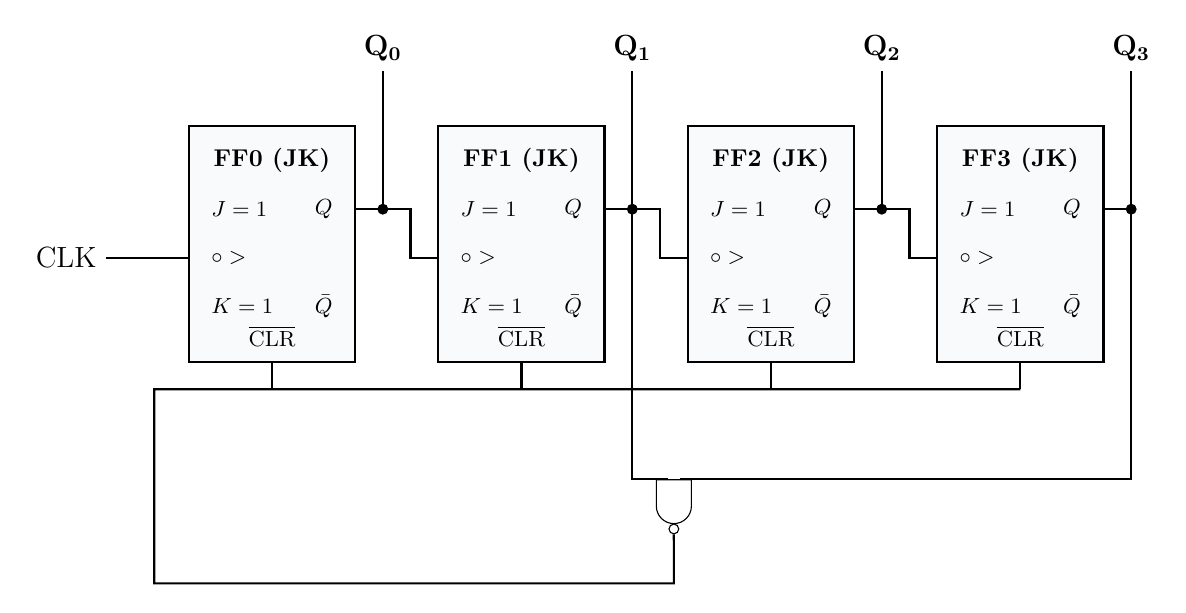
\begin{tikzpicture}[scale=0.88, transform shape]
  % 4 JK Flip Flops
  \foreach \i in {0,1,2,3} {
    \draw[thick, fill=boxbg] ({3.6*\i}, 0) rectangle ({3.6*\i + 2.4}, 3.4);
    \node at ({3.6*\i + 1.2}, 2.9) {\textbf{FF\i\ (JK)}};
    \node[anchor=west] at ({3.6*\i + 0.2}, 2.2) {\small $J=1$};
    \node[anchor=west] at ({3.6*\i + 0.2}, 1.5) {\small $\circ>$};
    \node[anchor=west] at ({3.6*\i + 0.2}, 0.8) {\small $K=1$};
    \node[anchor=east] at ({3.6*\i + 2.2}, 2.2) {\small $Q$};
    \node[anchor=east] at ({3.6*\i + 2.2}, 0.8) {\small $\bar{Q}$};
    \node[anchor=south] at ({3.6*\i + 1.2}, 0.1) {\small $\overline{\text{CLR}}$};

    % Output lines
    \filldraw[black] ({3.6*\i + 2.8}, 2.2) circle (2pt);
    \draw[thick] ({3.6*\i + 2.4}, 2.2) -- ({3.6*\i + 2.8}, 2.2) -- ({3.6*\i + 2.8}, 4.2) node[above] {\large $\mathbf{Q_\i}$};
  }

  % External Clock to FF0
  \draw[thick] (-1.2, 1.5) node[left] {\large $\mathbf{\text{CLK}}$} -- (0, 1.5);

  % Ripple clock connections (Q_i -> CLK_{i+1})
  \draw[thick] (2.8, 2.2) -- (3.2, 2.2) |- (3.6, 1.5);
  \draw[thick] (6.4, 2.2) -- (6.8, 2.2) |- (7.2, 1.5);
  \draw[thick] (10.0, 2.2) -- (10.4, 2.2) |- (10.8, 1.5);

  % NAND Reset Gate
  \node[nand gate US, draw, logic gate inputs=nn, rotate=-90] (nandRst) at (7.0, -2.0) {};
  \draw[thick] (13.6, 2.2) -- (13.6, -1.2) |- (nandRst.input 1); % Q3
  \draw[thick] (6.4, 2.2) -- (6.4, -1.2) |- (nandRst.input 2);  % Q1

  % Reset Bus to CLR pins
  \draw[thick] (nandRst.output) -- (7.0, -3.2) -- (-0.5, -3.2) -- (-0.5, -0.4) -- (12.0, -0.4);
  \foreach \i in {0,1,2,3} {
    \draw[thick] ({3.6*\i + 1.2}, -0.4) -- ({3.6*\i + 1.2}, 0);
  }
\end{tikzpicture}
\end{schematicbox}

\begin{answerbox}
The asynchronous BCD counter cycles through states $0000 \to 0001 \to \dots \to 1001 \to (1010 \text{ glitch}) \xrightarrow{\overline{\text{CLR}}=0} 0000$, implementing a stable Mod-10 frequency divider.
\end{answerbox}

\vspace{0.6cm}

% =========================================================================
% QUESTION 10
% =========================================================================
\subsection{Question 10: Synchronous Mod-10 UP Counter Schematic [7 Marks]}
\begin{questionbox}{Problem Statement (2083 Baishakh, Q10)}
Design the synchronous mod-10 up counter using T flip-flop and draw its timing diagram also.
\end{questionbox}

\paragraph{1. State Transition and T Excitation Table ($T = Q_n \oplus Q_{n+1}$):}
\begin{center}
\begin{tabular}{|c|cccc|cccc|cccc|}
\hline
\textbf{State} & \multicolumn{4}{c|}{\textbf{Present State}} & \multicolumn{4}{c|}{\textbf{Next State}} & \multicolumn{4}{c|}{\textbf{T Inputs}} \\
& $Q_3$ & $Q_2$ & $Q_1$ & $Q_0$ & $Q_3^+$ & $Q_2^+$ & $Q_1^+$ & $Q_0^+$ & $\mathbf{T_3}$ & $\mathbf{T_2}$ & $\mathbf{T_1}$ & $\mathbf{T_0}$ \\ \hline
0 & 0 & 0 & 0 & 0 & 0 & 0 & 0 & 1 & 0 & 0 & 0 & 1 \\ \hline
1 & 0 & 0 & 0 & 1 & 0 & 0 & 1 & 0 & 0 & 0 & 1 & 1 \\ \hline
2 & 0 & 0 & 1 & 0 & 0 & 0 & 1 & 1 & 0 & 0 & 0 & 1 \\ \hline
3 & 0 & 0 & 1 & 1 & 0 & 1 & 0 & 0 & 0 & 1 & 1 & 1 \\ \hline
4 & 0 & 1 & 0 & 0 & 0 & 1 & 0 & 1 & 0 & 0 & 0 & 1 \\ \hline
5 & 0 & 1 & 0 & 1 & 0 & 1 & 1 & 0 & 0 & 0 & 1 & 1 \\ \hline
6 & 0 & 1 & 1 & 0 & 0 & 1 & 1 & 1 & 0 & 0 & 0 & 1 \\ \hline
7 & 0 & 1 & 1 & 1 & 1 & 0 & 0 & 0 & 1 & 1 & 1 & 1 \\ \hline
8 & 1 & 0 & 0 & 0 & 1 & 0 & 0 & 1 & 0 & 0 & 0 & 1 \\ \hline
9 & 1 & 0 & 0 & 1 & 0 & 0 & 0 & 0 & 1 & 0 & 0 & 1 \\ \hline
\end{tabular}
\end{center}
(Unused states 10 to 15 are treated as Don't Cares $X$).

\paragraph{2. K-Map Derivations for T Inputs:}
\begin{itemize}
  \item $\mathbf{T_0 = 1}$ ($Q_0$ toggles on every single clock pulse).
  \item $\mathbf{T_1 = \bar{Q}_3 Q_0}$ ($Q_1$ toggles when $Q_0=1$ except when transitioning from 9 to 0).
  \item $\mathbf{T_2 = Q_1 Q_0}$ ($Q_2$ toggles when $Q_1 Q_0 = 1$).
  \item $\mathbf{T_3 = Q_2 Q_1 Q_0 + Q_3 Q_0}$ ($Q_3$ toggles at state 7 to become 1, and at state 9 to reset to 0).
\end{itemize}

\begin{schematicbox}{Synchronous Mod-10 UP Counter Logic Circuit}
\centering
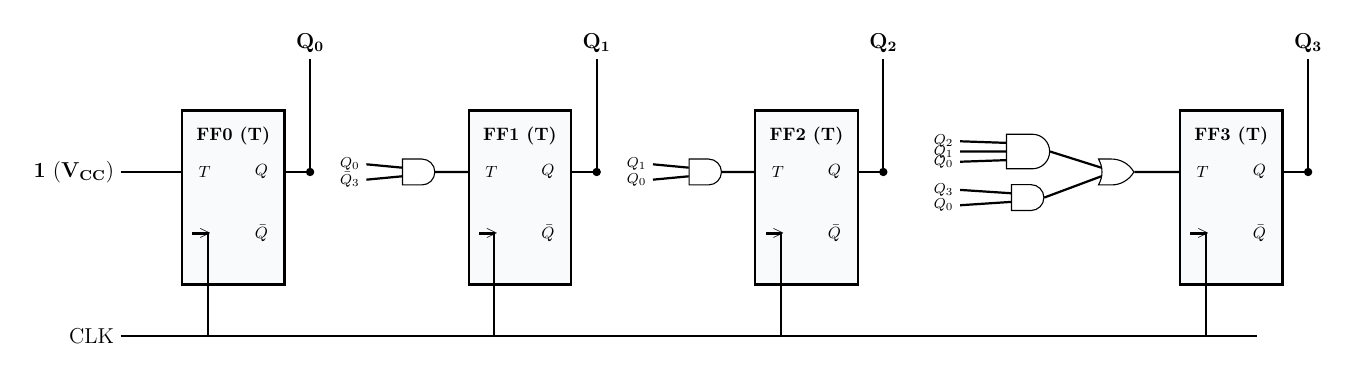
\begin{tikzpicture}[scale=0.65, transform shape]
  % 4 T Flip Flops (Width 2.0 each, wide inter-stage gaps)
  % FF0: x in [0, 2.0]
  % FF1: x in [5.6, 7.6]
  % FF2: x in [11.2, 13.2]
  % FF3: x in [19.5, 21.5]
  
  \foreach \i/\xpos in {0/0, 1/5.6, 2/11.2, 3/19.5} {
    \draw[thick, fill=boxbg] (\xpos, 0) rectangle (\xpos + 2.0, 3.4);
    \node at (\xpos + 1.0, 2.9) {\textbf{FF\i\ (T)}};
    \node[anchor=west] at (\xpos + 0.2, 2.2) {\small $T$};
    \node[anchor=west] at (\xpos + 0.2, 1.0) {\small $>$};
    \node[anchor=east] at (\xpos + 1.8, 2.2) {\small $Q$};
    \node[anchor=east] at (\xpos + 1.8, 1.0) {\small $\bar{Q}$};

    % Output pins Q_i
    \filldraw[black] (\xpos + 2.5, 2.2) circle (2pt);
    \draw[thick] (\xpos + 2.0, 2.2) -- (\xpos + 2.5, 2.2) -- (\xpos + 2.5, 4.4) node[above] {\large $\mathbf{Q_\i}$};
  }

  % T0 = 1 (VCC)
  \draw[thick] (-1.2, 2.2) node[left] {\large $\mathbf{1\ (V_{CC})}$} -- (0, 2.2);

  % Common Synchronous Clock Rail
  \draw[thick] (-1.2, -1.0) node[left] {\large $\mathbf{\text{CLK}}$} -- (21.0, -1.0);
  \foreach \xpos in {0, 5.6, 11.2, 19.5} {
    \draw[thick] (\xpos + 0.5, -1.0) -- (\xpos + 0.5, 1.0) -- (\xpos + 0.2, 1.0);
  }

  % T1 Gate = Q0 . Q3_bar (placed at x = 4.6 in gap [2.0, 5.6])
  \node[and gate US, draw, logic gate inputs=nn] (andT1) at (4.6, 2.2) {};
  \draw[thick] (3.6, 2.35) node[left] {\footnotesize $Q_0$} -- (andT1.input 1);
  \draw[thick] (3.6, 2.05) node[left] {\footnotesize $\bar{Q}_3$} -- (andT1.input 2);
  \draw[thick] (andT1.output) -- (5.6, 2.2);

  % T2 Gate = Q1 . Q0 (placed at x = 10.2 in gap [7.6, 11.2])
  \node[and gate US, draw, logic gate inputs=nn] (andT2) at (10.2, 2.2) {};
  \draw[thick] (9.2, 2.35) node[left] {\footnotesize $Q_1$} -- (andT2.input 1);
  \draw[thick] (9.2, 2.05) node[left] {\footnotesize $Q_0$} -- (andT2.input 2);
  \draw[thick] (andT2.output) -- (11.2, 2.2);

  % T3 Gates: andT3a, andT3b + orT3 (placed in wide gap [13.2, 19.5])
  \node[and gate US, draw, logic gate inputs=nnn] (andT3a) at (16.5, 2.6) {};
  \node[and gate US, draw, logic gate inputs=nn] (andT3b) at (16.5, 1.7) {};
  \node[or gate US, draw, logic gate inputs=nn] (orT3) at (18.2, 2.2) {};
  
  \draw[thick] (15.2, 2.8) node[left] {\footnotesize $Q_2$} -- (andT3a.input 1);
  \draw[thick] (15.2, 2.6) node[left] {\footnotesize $Q_1$} -- (andT3a.input 2);
  \draw[thick] (15.2, 2.4) node[left] {\footnotesize $Q_0$} -- (andT3a.input 3);
  
  \draw[thick] (15.2, 1.85) node[left] {\footnotesize $Q_3$} -- (andT3b.input 1);
  \draw[thick] (15.2, 1.55) node[left] {\footnotesize $Q_0$} -- (andT3b.input 2);
  
  \draw[thick] (andT3a.output) -- (orT3.input 1);
  \draw[thick] (andT3b.output) -- (orT3.input 2);
  \draw[thick] (orT3.output) -- (19.5, 2.2);
\end{tikzpicture}
\end{schematicbox}

\begin{answerbox}
$$\mathbf{T_0 = 1, \quad T_1 = \bar{Q}_3 Q_0, \quad T_2 = Q_1 Q_0, \quad T_3 = Q_2 Q_1 Q_0 + Q_3 Q_0}$$
\end{answerbox}

\vspace{0.6cm}

% =========================================================================
% QUESTION 11
% =========================================================================
\subsection{Question 11: Synchronous FSM Sequence Detector '011' [7 Marks]}
\begin{questionbox}{Problem Statement (2083 Baishakh, Q11)}
Design a synchronous sequential machine that has 1-bit serial input $X$ and output $Z$ which will be high when the input contains the message `011' (Use T Flip-Flop).
\end{questionbox}

\paragraph{1. State Definitions and State Diagram (Mealy Model):}
\begin{itemize}
  \item $S_0 (00)$: Reset state / No relevant bit detected.
  \item $S_1 (01)$: Sequence `0' detected.
  \item $S_2 (10)$: Sequence `01' detected.
  \item When in $S_2$ and next bit $X=1 \implies$ `011' detected $\implies Z=1$, next state $S_0$.
\end{itemize}

\begin{schematicbox}{State Transition Automaton for '011' Sequence Detector}
\centering
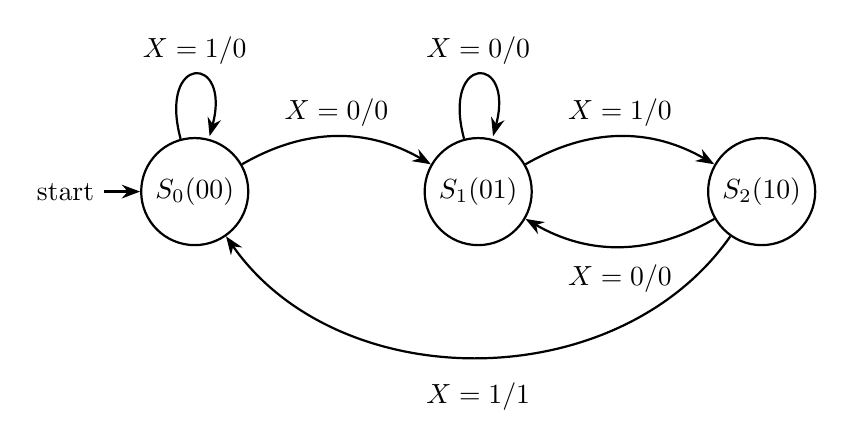
\begin{tikzpicture}[->, >=Stealth, auto, node distance=3.6cm, thick]
  \node[state, initial] (S0) {$S_0 (00)$};
  \node[state] (S1) [right of=S0] {$S_1 (01)$};
  \node[state] (S2) [right of=S1] {$S_2 (10)$};

  \path (S0) edge [loop above] node {$X=1 / 0$} (S0)
             edge [bend left] node {$X=0 / 0$} (S1)
        (S1) edge [loop above] node {$X=0 / 0$} (S1)
             edge [bend left] node {$X=1 / 0$} (S2)
        (S2) edge [bend left=55] node[below=2mm] {$X=1 / 1$} (S0)
             edge [bend left] node[below=1mm] {$X=0 / 0$} (S1);
\end{tikzpicture}
\end{schematicbox}

\paragraph{2. State Transition and Excitation Table for T Flip-Flops ($A, B$):}
\begin{center}
\begin{tabular}{|cc|c|cc|c|cc|}
\hline
\multicolumn{2}{|c|}{\textbf{Present State}} & \textbf{Input} & \multicolumn{2}{c|}{\textbf{Next State}} & \textbf{Output} & \multicolumn{2}{c|}{\textbf{T Inputs}} \\
$A$ & $B$ & $X$ & $A^+$ & $B^+$ & $\mathbf{Z}$ & $\mathbf{T_A}$ & $\mathbf{T_B}$ \\ \hline
0 & 0 & 0 & 0 & 1 & 0 & 0 & 1 \\ \hline
0 & 0 & 1 & 0 & 0 & 0 & 0 & 0 \\ \hline
0 & 1 & 0 & 0 & 1 & 0 & 0 & 0 \\ \hline
0 & 1 & 1 & 1 & 0 & 0 & 1 & 1 \\ \hline
1 & 0 & 0 & 0 & 1 & 0 & 1 & 1 \\ \hline
1 & 0 & 1 & 0 & 0 & 1 & 1 & 0 \\ \hline
1 & 1 & 0 & $X$ & $X$ & $X$ & $X$ & $X$ \\ \hline
1 & 1 & 1 & $X$ & $X$ & $X$ & $X$ & $X$ \\ \hline
\end{tabular}
\end{center}

\paragraph{3. Minimized Equations via K-Maps:}
\begin{align*}
T_A &= A + BX \\
T_B &= \bar{A}\bar{B}\bar{X} + BX + A\bar{X} \\
Z &= AX
\end{align*}

\begin{schematicbox}{Synchronous FSM Circuit Realization Using T Flip-Flops}
\centering
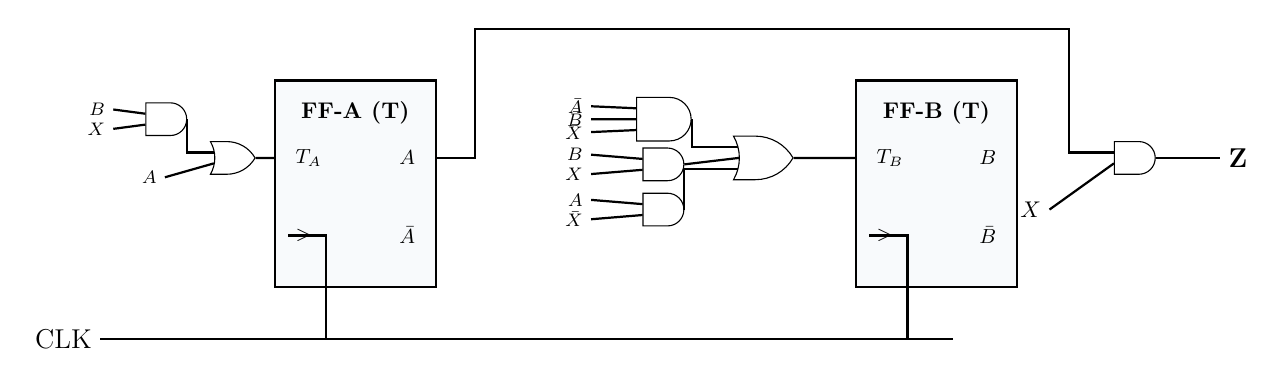
\begin{tikzpicture}[scale=0.82, transform shape]
  % Flip-Flop A (x in [0.5, 3.0]) and Flip-Flop B (x in [9.5, 12.0]) -> 6.5cm wide gap in middle!
  \draw[thick, fill=boxbg] (0.5, 0) rectangle (3.0, 3.2);
  \node at (1.75, 2.7) {\textbf{FF-A (T)}};
  \node[anchor=west] at (0.7, 2.0) {\small $T_A$};
  \node[anchor=west] at (0.7, 0.8) {\small $>$};
  \node[anchor=east] at (2.8, 2.0) {\small $A$};
  \node[anchor=east] at (2.8, 0.8) {\small $\bar{A}$};

  \draw[thick, fill=boxbg] (9.5, 0) rectangle (12.0, 3.2);
  \node at (10.75, 2.7) {\textbf{FF-B (T)}};
  \node[anchor=west] at (9.7, 2.0) {\small $T_B$};
  \node[anchor=west] at (9.7, 0.8) {\small $>$};
  \node[anchor=east] at (11.8, 2.0) {\small $B$};
  \node[anchor=east] at (11.8, 0.8) {\small $\bar{B}$};

  % Common Clock
  \draw[thick] (-2.2, -0.8) node[left] {\large $\mathbf{\text{CLK}}$} -- (11.0, -0.8);
  \draw[thick] (1.3, -0.8) -- (1.3, 0.8) -- (0.7, 0.8);
  \draw[thick] (10.3, -0.8) -- (10.3, 0.8) -- (9.7, 0.8);

  % Combinational Gates for T_A = A + BX (on the left, x in [-2.0, 0.5])
  \node[and gate US, draw, logic gate inputs=nn] (andTA) at (-1.2, 2.6) {};
  \node[or gate US, draw, logic gate inputs=nn] (orTA) at (-0.2, 2.0) {};
  \draw[thick] (-2.0, 2.75) node[left] {\footnotesize $B$} -- (andTA.input 1);
  \draw[thick] (-2.0, 2.45) node[left] {\footnotesize $X$} -- (andTA.input 2);
  \draw[thick] (andTA.output) |- (orTA.input 1);
  \draw[thick] (-1.2, 1.7) node[left] {\footnotesize $A$} -- (orTA.input 2);
  \draw[thick] (orTA.output) -- (0.5, 2.0);

  % Combinational Gates for T_B = \bar{A}\bar{B}\bar{X} + BX + A\bar{X} (centered in the wide 6.5cm gap at x=6.0 to 8.5)
  \node[and gate US, draw, logic gate inputs=nnn] (andTB1) at (6.5, 2.6) {};
  \node[and gate US, draw, logic gate inputs=nn] (andTB2) at (6.5, 1.9) {};
  \node[and gate US, draw, logic gate inputs=nn] (andTB3) at (6.5, 1.2) {};
  \node[or gate US, draw, logic gate inputs=nnn] (orTB) at (8.0, 2.0) {};
  
  \draw[thick] (5.4, 2.8) node[left] {\footnotesize $\bar{A}$} -- (andTB1.input 1);
  \draw[thick] (5.4, 2.6) node[left] {\footnotesize $\bar{B}$} -- (andTB1.input 2);
  \draw[thick] (5.4, 2.4) node[left] {\footnotesize $\bar{X}$} -- (andTB1.input 3);
  
  \draw[thick] (5.4, 2.05) node[left] {\footnotesize $B$} -- (andTB2.input 1);
  \draw[thick] (5.4, 1.75) node[left] {\footnotesize $X$} -- (andTB2.input 2);
  
  \draw[thick] (5.4, 1.35) node[left] {\footnotesize $A$} -- (andTB3.input 1);
  \draw[thick] (5.4, 1.05) node[left] {\footnotesize $\bar{X}$} -- (andTB3.input 2);
  
  \draw[thick] (andTB1.output) |- (orTB.input 1);
  \draw[thick] (andTB2.output) -- (orTB.input 2);
  \draw[thick] (andTB3.output) |- (orTB.input 3);
  \draw[thick] (orTB.output) -- (9.5, 2.0);

  % Output Z = A . X (placed to the right of FF-B at x=13.8)
  \node[and gate US, draw, logic gate inputs=nn] (andZ) at (13.8, 2.0) {};
  \draw[thick] (3.0, 2.0) -- (3.6, 2.0) -- (3.6, 4.0) -- (12.8, 4.0) |- (andZ.input 1);
  \draw[thick] (12.5, 1.2) node[left] {$X$} -- (andZ.input 2);
  \draw[thick] (andZ.output) -- ++(1.0, 0) node[right] {\large $\mathbf{Z}$};
\end{tikzpicture}
\end{schematicbox}

\begin{answerbox}
$$\mathbf{T_A = A + BX, \quad T_B = \bar{A}\bar{B}\bar{X} + BX + A\bar{X}, \quad Z = AX}$$
\end{answerbox}

\vspace{0.6cm}

% =========================================================================
% QUESTION 12
% =========================================================================
\subsection{Question 12: Characteristics of Digital Logic Families [4 Marks]}
\begin{questionbox}{Problem Statement (2083 Baishakh, Q12)}
Explain about the main characteristics of digital logic families.
\end{questionbox}

The performance and suitability of digital integrated circuit (IC) families are evaluated based on the following key operational parameters:

\begin{enumerate}[leftmargin=*]
  \item \textbf{Propagation Delay ($t_{pd}$):} The average time elapsed between the application of an input logic transition and the resulting output logic transition:
  \[
  t_{pd} = \frac{t_{pLH} + t_{pHL}}{2}
  \]
  where $t_{pLH}$ is the low-to-high delay and $t_{pHL}$ is the high-to-low delay. Lower propagation delay indicates higher operating speed.

  \item \textbf{Power Dissipation ($P_D$):} The DC power consumed by the logic gate during static and dynamic operation, expressed in milliwatts (mW) or microwatts ($\mu$W):
  \[
  P_D = V_{CC} \times I_{CC(\text{avg})}
  \]

  \item \textbf{Speed-Power Product (Figure of Merit):} The product of propagation delay and power dissipation:
  \[
  \text{SPP} = t_{pd} \times P_D \quad (\text{expressed in picojoules, pJ})
  \]
  A lower SPP value signifies superior overall technological performance.

  \item \textbf{Noise Margins ($NM_H$ and $NM_L$):} The maximum allowable unwanted noise voltage superimposed on the input without causing an erroneous output change:
  \[
  NM_H = V_{OH(\min)} - V_{IH(\min)}, \qquad NM_L = V_{IL(\max)} - V_{OL(\max)}
  \]

  \item \textbf{Fan-Out and Fan-In:}
  \begin{itemize}
    \item \textbf{Fan-Out:} Maximum number of standard logic gate inputs of the same family that an output can reliably drive without exceeding current limits.
    \item \textbf{Fan-In:} Number of independent input signals that a single gate can accommodate without degradation.
  \end{itemize}

  \item \textbf{Operating Temperature Range:} Standard commercial grade ($0^\circ\text{C}$ to $70^\circ\text{C}$) versus military grade ($-55^\circ\text{C}$ to $+125^\circ\text{C}$).
\end{enumerate}

\paragraph{Comparative Summary of Major Digital Logic Families:}
\begin{center}
\small
\begin{tabular}{@{}lcccc@{}}
\toprule
\textbf{Parameter} & \textbf{Standard TTL (7400)} & \textbf{Schottky TTL (74S)} & \textbf{CMOS (74HC)} & \textbf{ECL (10K)} \\
\midrule
\textbf{Propagation Delay ($t_{pd}$)} & $10\text{ ns}$ & $3\text{ ns}$ & $8\text{ ns}$ & $1\text{ ns}$ \\
\textbf{Power Dissipation / Gate} & $10\text{ mW}$ & $20\text{ mW}$ & $0.001\text{ mW (static)}$ & $25\text{ mW}$ \\
\textbf{Speed-Power Product (SPP)} & $100\text{ pJ}$ & $60\text{ pJ}$ & $0.008\text{ pJ}$ & $25\text{ pJ}$ \\
\textbf{Noise Margin ($NM$)} & $0.4\text{ V}$ & $0.3\text{ V}$ & $> 1.0\text{ V}$ & $0.25\text{ V}$ \\
\textbf{Fan-Out} & 10 & 20 & $> 50$ & 25 \\
\bottomrule
\end{tabular}
\end{center}

\begin{answerbox}
Digital logic families are comprehensively characterized by speed ($t_{pd}$), power consumption ($P_D$), noise margins ($NM_H, NM_L$), fan-out, and the Speed-Power Product figure of merit.
\end{answerbox}

\chapter{2082 Bhadra Examination Solutions}

\section*{Examination Overview}
\begin{tabular}{@{}ll@{}}
\textbf{Level:} Bachelor in Engineering (BE) & \textbf{Full Marks:} 60 \\
\textbf{Programme:} BEI, BCT & \textbf{Pass Marks:} 24 \\
\textbf{Year / Part:} I / II & \textbf{Time:} 3 Hours \\
\textbf{Subject:} Digital Logic (ENEX 152 / EX 152) & \textbf{Examination Type:} Regular / Back \\
\end{tabular}

\vspace{0.6cm}
\hrule
\vspace{0.6cm}

% =========================================================================
% QUESTION 1
% =========================================================================
\subsection{Question 1: Binary to Gray Code Conversion [2 + 2 = 4 Marks]}
\begin{questionbox}{Problem Statement (2082 Bhadra, Q1)}
Convert the following binary codes to gray codes:
\begin{enumerate}[label=(\alph*)]
  \item $(101101)_2$
  \item $(110001)_2$
\end{enumerate}
\end{questionbox}

\paragraph{Conversion Algorithm:}
Given an $n$-bit binary word $B = b_{n-1} b_{n-2} \dots b_1 b_0$ and target Gray code $G = g_{n-1} g_{n-2} \dots g_1 g_0$:
\begin{enumerate}
  \item $g_{n-1} = b_{n-1}$ (The Most Significant Bit remains unchanged).
  \item $g_i = b_{i+1} \oplus b_i$ for each subsequent bit position $i = n-2, n-3, \dots, 0$.
\end{enumerate}

\paragraph{Part (a): Conversion of $(101101)_2$}
Given $b_5 b_4 b_3 b_2 b_1 b_0 = 101101_2$:
\begin{itemize}
  \item $g_5 = b_5 = 1$
  \item $g_4 = b_5 \oplus b_4 = 1 \oplus 0 = 1$
  \item $g_3 = b_4 \oplus b_3 = 0 \oplus 1 = 1$
  \item $g_2 = b_3 \oplus b_2 = 1 \oplus 1 = 0$
  \item $g_1 = b_2 \oplus b_1 = 1 \oplus 0 = 1$
  \item $g_0 = b_1 \oplus b_0 = 0 \oplus 1 = 1$
\end{itemize}
Thus, $(101101)_2 = (111011)_{\text{Gray}}$.

\paragraph{Part (b): Conversion of $(110001)_2$}
Given $b_5 b_4 b_3 b_2 b_1 b_0 = 110001_2$:
\begin{itemize}
  \item $g_5 = b_5 = 1$
  \item $g_4 = b_5 \oplus b_4 = 1 \oplus 1 = 0$
  \item $g_3 = b_4 \oplus b_3 = 1 \oplus 0 = 1$
  \item $g_2 = b_3 \oplus b_2 = 0 \oplus 0 = 0$
  \item $g_1 = b_2 \oplus b_1 = 0 \oplus 0 = 0$
  \item $g_0 = b_1 \oplus b_0 = 0 \oplus 1 = 1$
\end{itemize}
Thus, $(110001)_2 = (101001)_{\text{Gray}}$.

\begin{answerbox}
\begin{align*}
\text{(a)}\quad (101101)_2 &= \mathbf{(111011)_{\text{Gray}}} \\
\text{(b)}\quad (110001)_2 &= \mathbf{(101001)_{\text{Gray}}}
\end{align*}
\end{answerbox}

\vspace{0.6cm}

% =========================================================================
% QUESTION 2
% =========================================================================
\subsection{Question 2: 2's Complement \& BCD Addition [1 + 2 = 3 Marks]}
\begin{questionbox}{Problem Statement (2082 Bhadra, Q2)}
What is 2's complement representation? Perform BCD addition of $(23)_{10} + (48)_{10}$.
\end{questionbox}

\paragraph{Part (a): 2's Complement Representation [1 Mark]}
2's complement is the standard system used in digital computers to represent signed integers. For an $n$-bit binary number $X$:
\[
\text{2's Complement of } X = 2^n - X = (\text{1's Complement of } X) + 1
\]
\textbf{Key Advantages:}
\begin{itemize}
  \item Unambiguous representation of zero (single representation $0000_2$, unlike 1's complement which has $+0$ and $-0$).
  \item Simplifies hardware arithmetic: subtraction $A - B$ is performed as addition $A + (\text{2's comp of } B)$ using standard binary adder circuits.
\end{itemize}

\paragraph{Part (b): BCD Addition of $23_{10} + 48_{10}$ [2 Marks]}
In BCD (8421 code), each decimal digit is encoded into 4 bits ($0000_2$ to $1001_2$). If the sum of any decade exceeds $9$ ($1001_2$) or produces a carry, a correction factor of $+6$ ($0110_2$) must be added.
\begin{itemize}
  \item Represent numbers in BCD:
  \[
  23_{10} = \mathbf{0010\ 0011}_{\text{BCD}}, \qquad 48_{10} = \mathbf{0100\ 1000}_{\text{BCD}}
  \]
  \item \textbf{Step 1: Add Lower Decade (Units):}
  \[
  \begin{array}{r@{\quad}l}
    0011 & (3_{10}) \\
  +\ 1000 & (8_{10}) \\
  \hline
    1011_2 & (11_{10} > 9 \implies \text{Invalid BCD})
  \end{array}
  \]
  \item \textbf{Step 2: Add Correction Factor ($+0110_2$):}
  \[
  \begin{array}{r@{\quad}l}
    1011 & \\
  +\ 0110 & (+6_{10}) \\
  \hline
    \mathbf{0001}_2 & \text{with Carry Out } C_{\text{out}} = 1 \text{ to Upper Decade}
  \end{array}
  \]
  \item \textbf{Step 3: Add Upper Decade (Tens) including Carry In:}
  \[
  \begin{array}{r@{\quad}l}
    0010 & (2_{10}) \\
    0100 & (4_{10}) \\
  +\ 0001 & (\text{Carry in} = 1) \\
  \hline
    \mathbf{0111}_2 & (7_{10} \le 9 \implies \text{Valid BCD})
  \end{array}
  \]
\end{itemize}

\begin{answerbox}
$$(23)_{10} + (48)_{10} = \mathbf{0111\ 0001_{\text{BCD}}} = (71)_{10}$$
\end{answerbox}

\vspace{0.6cm}

% =========================================================================
% QUESTION 3
% =========================================================================
\subsection{Question 3: De Morgan's Theorem with Diagrams [4 Marks]}
\begin{questionbox}{Problem Statement (2082 Bhadra, Q3)}
State and explain De Morgan's Theorem with truth table and necessary diagrams.
\end{questionbox}

\paragraph{1. First Theorem (NAND-to-Inverted-OR Equivalence):}
The complement of a product of variables is equal to the sum of the complements of the variables:
\[
\overline{A \cdot B} = \bar{A} + \bar{B}
\]

\paragraph{2. Second Theorem (NOR-to-Inverted-AND Equivalence):}
The complement of a sum of variables is equal to the product of the complements of the variables:
\[
\overline{A + B} = \bar{A} \cdot \bar{B}
\]

\paragraph{Truth Table Verification:}
\begin{center}
\begin{tabular}{|cc|cc|c|c||c|c|}
\hline
$A$ & $B$ & $\bar{A}$ & $\bar{B}$ & $\overline{A \cdot B}$ & $\bar{A} + \bar{B}$ & $\overline{A + B}$ & $\bar{A} \cdot \bar{B}$ \\ \hline
0 & 0 & 1 & 1 & \textbf{1} & \textbf{1} & \textbf{1} & \textbf{1} \\ \hline
0 & 1 & 1 & 0 & \textbf{1} & \textbf{1} & \textbf{0} & \textbf{0} \\ \hline
1 & 0 & 0 & 1 & \textbf{1} & \textbf{1} & \textbf{0} & \textbf{0} \\ \hline
1 & 1 & 0 & 0 & \textbf{0} & \textbf{0} & \textbf{0} & \textbf{0} \\ \hline
\end{tabular}
\end{center}
Columns 5 and 6 are identical, verifying Theorem 1. Columns 7 and 8 are identical, verifying Theorem 2.

\begin{schematicbox}{De Morgan's Equivalent Logic Gate Pairs}
\centering
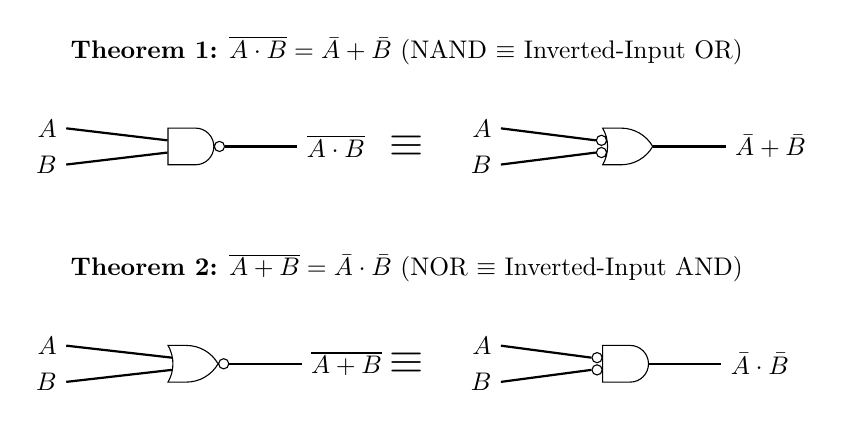
\begin{tikzpicture}[scale=0.92, transform shape]
  % Theorem 1: NAND == Bubbled OR
  \node[nand gate US, draw, logic gate inputs=nn] (nand1) at (2.5, 2.2) {};
  \draw[thick] (0.8, 2.45) node[left] {$A$} -- (nand1.input 1);
  \draw[thick] (0.8, 1.95) node[left] {$B$} -- (nand1.input 2);
  \draw[thick] (nand1.output) -- ++(1.0, 0) node[right] {$\overline{A \cdot B}$};

  \node at (5.5, 2.2) {\LARGE $\equiv$};

  \node[or gate US, draw, logic gate inputs=ii, scale=1.0] (bubOR) at (8.5, 2.2) {};
  \draw[thick] (6.8, 2.45) node[left] {$A$} -- (bubOR.input 1);
  \draw[thick] (6.8, 1.95) node[left] {$B$} -- (bubOR.input 2);
  \draw[thick] (bubOR.output) -- ++(1.0, 0) node[right] {$\bar{A} + \bar{B}$};
  \node[above] at (5.5, 3.2) {\textbf{Theorem 1:} $\overline{A \cdot B} = \bar{A} + \bar{B}$ (NAND $\equiv$ Inverted-Input OR)};

  % Theorem 2: NOR == Bubbled AND
  \node[nor gate US, draw, logic gate inputs=nn] (nor1) at (2.5, -0.8) {};
  \draw[thick] (0.8, -0.55) node[left] {$A$} -- (nor1.input 1);
  \draw[thick] (0.8, -1.05) node[left] {$B$} -- (nor1.input 2);
  \draw[thick] (nor1.output) -- ++(1.0, 0) node[right] {$\overline{A + B}$};

  \node at (5.5, -0.8) {\LARGE $\equiv$};

  \node[and gate US, draw, logic gate inputs=ii, scale=1.0] (bubAND) at (8.5, -0.8) {};
  \draw[thick] (6.8, -0.55) node[left] {$A$} -- (bubAND.input 1);
  \draw[thick] (6.8, -1.05) node[left] {$B$} -- (bubAND.input 2);
  \draw[thick] (bubAND.output) -- ++(1.0, 0) node[right] {$\bar{A} \cdot \bar{B}$};
  \node[above] at (5.5, 0.2) {\textbf{Theorem 2:} $\overline{A + B} = \bar{A} \cdot \bar{B}$ (NOR $\equiv$ Inverted-Input AND)};
\end{tikzpicture}
\end{schematicbox}

\begin{answerbox}
De Morgan's Laws establish dual relationships between AND and OR operations through inversion: $\mathbf{\overline{A \cdot B} = \bar{A} + \bar{B}}$ and $\mathbf{\overline{A + B} = \bar{A} \cdot \bar{B}}$.
\end{answerbox}

\vspace{0.6cm}

% =========================================================================
% QUESTION 4
% =========================================================================
\subsection{Question 4: K-Map with Don't Cares \& Circuit [5 Marks]}
\begin{questionbox}{Problem Statement (2082 Bhadra, Q4)}
Minimize the function $F(A, B, C, D) = \sum m(0,1,2,4,7,8,9,10,12,15) + d(5,11,13)$ using K-Map and realize it with suitable logic gates.
\end{questionbox}

\paragraph{1. K-Map Plotting (4-Variable K-Map):}
\begin{center}
\begin{tabular}{|c|c|c|c|c|}
\hline
$AB \ \backslash \ CD$ & \textbf{00} & \textbf{01} & \textbf{11} & \textbf{10} \\ \hline
\textbf{00} & $\mathbf{1}\ (m_0)$ & $\mathbf{1}\ (m_1)$ & $0\ (m_3)$ & $\mathbf{1}\ (m_2)$ \\ \hline
\textbf{01} & $\mathbf{1}\ (m_4)$ & $\mathbf{X}\ (d_5)$ & $\mathbf{1}\ (m_7)$ & $0\ (m_6)$ \\ \hline
\textbf{11} & $\mathbf{1}\ (m_{12})$ & $\mathbf{X}\ (d_{13})$ & $\mathbf{1}\ (m_{15})$ & $0\ (m_{14})$ \\ \hline
\textbf{10} & $\mathbf{1}\ (m_8)$ & $\mathbf{1}\ (m_9)$ & $\mathbf{X}\ (d_{11})$ & $\mathbf{1}\ (m_{10})$ \\ \hline
\end{tabular}
\end{center}

\paragraph{2. Grouping Analysis:}
\begin{enumerate}
  \item \textbf{Octet 1 (Columns $CD=00$ and $CD=01$):} \\
  Cells $(m_0, m_1, m_4, d_5, m_{12}, d_{13}, m_8, m_9) \implies \mathbf{\bar{C}}$.
  \item \textbf{Quad 2 (Center and Column 11):} \\
  Cells $(d_5, m_7, d_{13}, m_{15}) \implies \mathbf{BD}$.
  \item \textbf{Quad 3 (Four Corners):} \\
  Cells $(m_0, m_2, m_8, m_{10}) \implies \mathbf{\bar{B}\bar{D}}$.
\end{enumerate}

\paragraph{Minimal Sum of Products (SOP):}
\[
F(A,B,C,D) = \bar{C} + BD + \bar{B}\bar{D}
\]
(Note that $BD + \bar{B}\bar{D} = \overline{B \oplus D} = B \odot D$, the XNOR equivalence).

\begin{schematicbox}{Logic Circuit Realization for Minimized $F(A,B,C,D) = \bar{C} + BD + \bar{B}\bar{D}$}
\centering
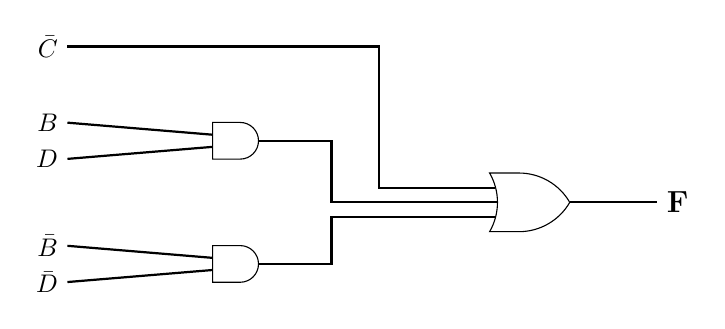
\begin{tikzpicture}[scale=0.92, transform shape]
  % Gates
  \node[and gate US, draw, logic gate inputs=nn] (and1) at (3.5, 2.5) {};
  \node[and gate US, draw, logic gate inputs=nn] (and2) at (3.5, 0.8) {};
  \node[or gate US, draw, logic gate inputs=nnn, scale=1.2] (orgate) at (7.5, 1.65) {};

  % Input connections to AND1 (B, D)
  \draw[thick] (1.2, 2.75) node[left] {$B$} -- (and1.input 1);
  \draw[thick] (1.2, 2.25) node[left] {$D$} -- (and1.input 2);

  % Input connections to AND2 (\bar{B}, \bar{D})
  \draw[thick] (1.2, 1.05) node[left] {$\bar{B}$} -- (and2.input 1);
  \draw[thick] (1.2, 0.55) node[left] {$\bar{D}$} -- (and2.input 2);

  % Direct \bar{C} line
  \draw[thick] (1.2, 3.8) node[left] {$\bar{C}$} -- (5.5, 3.8) |- (orgate.input 1);

  % AND outputs to OR
  \draw[thick] (and1.output) -- ++(1.0, 0) |- (orgate.input 2);
  \draw[thick] (and2.output) -- ++(1.0, 0) |- (orgate.input 3);

  % Final Output
  \draw[thick] (orgate.output) -- ++(1.2, 0) node[right] {\large $\mathbf{F}$};
\end{tikzpicture}
\end{schematicbox}

\begin{answerbox}
$$\mathbf{F(A,B,C,D) = \bar{C} + BD + \bar{B}\bar{D} = \bar{C} + (B \odot D)}$$
\end{answerbox}

\vspace{0.6cm}

% =========================================================================
% QUESTION 5
% =========================================================================
\subsection{Question 5: 3-Bit Magnitude Comparator Schematic [1 + 5 = 6 Marks]}
\begin{questionbox}{Problem Statement (2082 Bhadra, Q5)}
What is a magnitude comparator? Design a 3-bit magnitude comparator.
\end{questionbox}

\paragraph{Part (a): Definition of Magnitude Comparator [1 Mark]}
A \textbf{magnitude comparator} is a combinational logic circuit that compares two binary numbers $A$ and $B$, generating three mutually exclusive digital outputs indicating whether $A > B$, $A = B$, or $A < B$.

\paragraph{Part (b): Design of 3-Bit Magnitude Comparator [5 Marks]}
Let the two 3-bit input numbers be:
\[
A = (A_2 A_1 A_0)_2, \qquad B = (B_2 B_1 B_0)_2
\]
where $A_2, B_2$ are the Most Significant Bits (MSBs) and $A_0, B_0$ are the Least Significant Bits (LSBs).

\paragraph{1. Equality Condition ($A = B$):}
Two numbers are equal if and only if all corresponding bits are identical:
\[
x_i = A_i \odot B_i = A_i B_i + \bar{A}_i \bar{B}_i \quad \text{for } i = 0, 1, 2
\]
Therefore, the equality output $(A = B)$ is:
\[
\mathbf{(A = B) = x_2 \cdot x_1 \cdot x_0}
\]

\paragraph{2. Greater Than Condition ($A > B$):}
$A$ is strictly greater than $B$ if:
\begin{itemize}
  \item The MSB of $A$ is 1 and MSB of $B$ is 0 ($A_2 > B_2 \implies A_2 \bar{B}_2$), OR
  \item MSBs are equal ($x_2=1$) and $A_1 > B_1$ ($A_1 \bar{B}_1$), OR
  \item MSBs and middle bits are equal ($x_2 x_1 = 1$) and $A_0 > B_0$ ($A_0 \bar{B}_0$).
\end{itemize}
\[
\mathbf{(A > B) = A_2 \bar{B}_2 + x_2 A_1 \bar{B}_1 + x_2 x_1 A_0 \bar{B}_0}
\]

\paragraph{3. Less Than Condition ($A < B$):}
By symmetric logic:
\[
\mathbf{(A < B) = \bar{A}_2 B_2 + x_2 \bar{A}_1 B_1 + x_2 x_1 \bar{A}_0 B_0}
\]

\begin{schematicbox}{3-Bit Magnitude Comparator Logic Schematic}
\centering
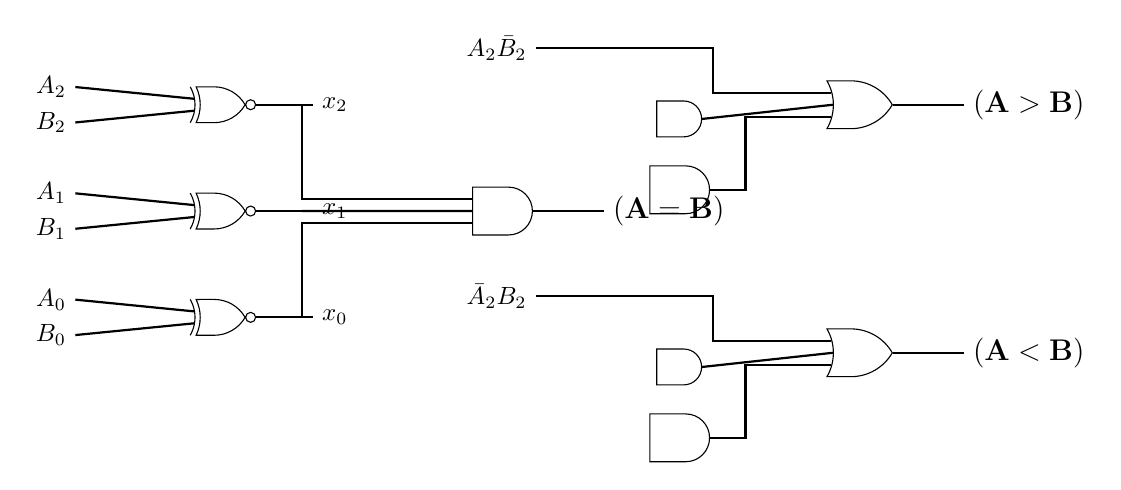
\begin{tikzpicture}[scale=0.9, transform shape]
  % XNOR gates for x2, x1, x0
  \node[xnor gate US, draw, logic gate inputs=nn] (xnor2) at (3.0, 5.0) {};
  \draw[thick] (1.0, 5.25) node[left] {$A_2$} -- (xnor2.input 1);
  \draw[thick] (1.0, 4.75) node[left] {$B_2$} -- (xnor2.input 2);
  \draw[thick] (xnor2.output) -- ++(0.8, 0) node[right] {$x_2$};

  \node[xnor gate US, draw, logic gate inputs=nn] (xnor1) at (3.0, 3.5) {};
  \draw[thick] (1.0, 3.75) node[left] {$A_1$} -- (xnor1.input 1);
  \draw[thick] (1.0, 3.25) node[left] {$B_1$} -- (xnor1.input 2);
  \draw[thick] (xnor1.output) -- ++(0.8, 0) node[right] {$x_1$};

  \node[xnor gate US, draw, logic gate inputs=nn] (xnor0) at (3.0, 2.0) {};
  \draw[thick] (1.0, 2.25) node[left] {$A_0$} -- (xnor0.input 1);
  \draw[thick] (1.0, 1.75) node[left] {$B_0$} -- (xnor0.input 2);
  \draw[thick] (xnor0.output) -- ++(0.8, 0) node[right] {$x_0$};

  % A = B AND Gate
  \node[and gate US, draw, logic gate inputs=nnn] (andEQ) at (7.0, 3.5) {};
  \draw[thick] (4.2, 5.0) |- (andEQ.input 1);
  \draw[thick] (4.2, 3.5) -- (andEQ.input 2);
  \draw[thick] (4.2, 2.0) |- (andEQ.input 3);
  \draw[thick] (andEQ.output) -- ++(1.0, 0) node[right] {\large $\mathbf{(A = B)}$};

  % A > B OR Gate and AND stages
  \node[or gate US, draw, logic gate inputs=nnn] (orGT) at (12.0, 5.0) {};
  \node[and gate US, draw, logic gate inputs=nn] (andGT1) at (9.5, 4.8) {};
  \node[and gate US, draw, logic gate inputs=nnn] (andGT2) at (9.5, 3.8) {};

  \draw[thick] (7.5, 5.8) node[left] {$A_2 \bar{B}_2$} -- ++(2.5, 0) |- (orGT.input 1);
  \draw[thick] (andGT1.output) -- (orGT.input 2);
  \draw[thick] (andGT2.output) -- ++(0.5, 0) |- (orGT.input 3);
  \draw[thick] (orGT.output) -- ++(1.0, 0) node[right] {\large $\mathbf{(A > B)}$};

  % A < B OR Gate and AND stages
  \node[or gate US, draw, logic gate inputs=nnn] (orLT) at (12.0, 1.5) {};
  \node[and gate US, draw, logic gate inputs=nn] (andLT1) at (9.5, 1.3) {};
  \node[and gate US, draw, logic gate inputs=nnn] (andLT2) at (9.5, 0.3) {};

  \draw[thick] (7.5, 2.3) node[left] {$\bar{A}_2 B_2$} -- ++(2.5, 0) |- (orLT.input 1);
  \draw[thick] (andLT1.output) -- (orLT.input 2);
  \draw[thick] (andLT2.output) -- ++(0.5, 0) |- (orLT.input 3);
  \draw[thick] (orLT.output) -- ++(1.0, 0) node[right] {\large $\mathbf{(A < B)}$};
\end{tikzpicture}
\end{schematicbox}

\begin{answerbox}
\begin{align*}
(A = B) &= x_2 x_1 x_0 \\
(A > B) &= A_2 \bar{B}_2 + x_2 A_1 \bar{B}_1 + x_2 x_1 A_0 \bar{B}_0 \\
(A < B) &= \bar{A}_2 B_2 + x_2 \bar{A}_1 B_1 + x_2 x_1 \bar{A}_0 B_0
\end{align*}
\end{answerbox}

\vspace{0.6cm}

% =========================================================================
% QUESTION 6
% =========================================================================
\subsection{Question 6: Full Adder Using Multiplexers [4 Marks]}
\begin{questionbox}{Problem Statement (2082 Bhadra, Q6)}
Implement a full adder circuit using Multiplexer.
\end{questionbox}

A full adder adds three 1-bit binary inputs: Augend ($A$), Addend ($B$), and Carry In ($C_{\text{in}}$). It generates Sum ($S$) and Carry Out ($C_{\text{out}}$).

\paragraph{Truth Table:}
\begin{center}
\begin{tabular}{|ccc||cc|}
\hline
$A$ & $B$ & $C_{\text{in}}$ & $\mathbf{S\ (Sum)}$ & $\mathbf{C_{\text{out}}\ (Carry)}$ \\ \hline
0 & 0 & 0 & 0 & 0 \\ \hline
0 & 0 & 1 & 1 & 0 \\ \hline
0 & 1 & 0 & 1 & 0 \\ \hline
0 & 1 & 1 & 0 & 1 \\ \hline
1 & 0 & 0 & 1 & 0 \\ \hline
1 & 0 & 1 & 0 & 1 \\ \hline
1 & 1 & 0 & 0 & 1 \\ \hline
1 & 1 & 1 & 1 & 1 \\ \hline
\end{tabular}
\end{center}
\[
S(A,B,C_{\text{in}}) = \sum m(1, 2, 4, 7), \qquad C_{\text{out}}(A,B,C_{\text{in}}) = \sum m(3, 5, 6, 7)
\]

\paragraph{Multiplexer Implementation using Two $4:1$ MUXes:}
Let select lines be $S_1 = A, S_0 = B$:
\begin{center}
\begin{tabular}{|c|c|c|c|}
\hline
\textbf{Select Inputs} $(A, B)$ & \textbf{Data Channel} & \textbf{Sum ($S$)} & \textbf{Carry Out ($C_{\text{out}}$)} \\ \hline
$00$ & $I_0$ & $C_{\text{in}}$ & $0\ (\text{GND})$ \\ \hline
$01$ & $I_1$ & $\bar{C}_{\text{in}}$ & $C_{\text{in}}$ \\ \hline
$10$ & $I_2$ & $\bar{C}_{\text{in}}$ & $C_{\text{in}}$ \\ \hline
$11$ & $I_3$ & $C_{\text{in}}$ & $1\ (V_{CC})$ \\ \hline
\end{tabular}
\end{center}

\begin{schematicbox}{Full Adder Implementation Using Two 4:1 Multiplexers}
\centering
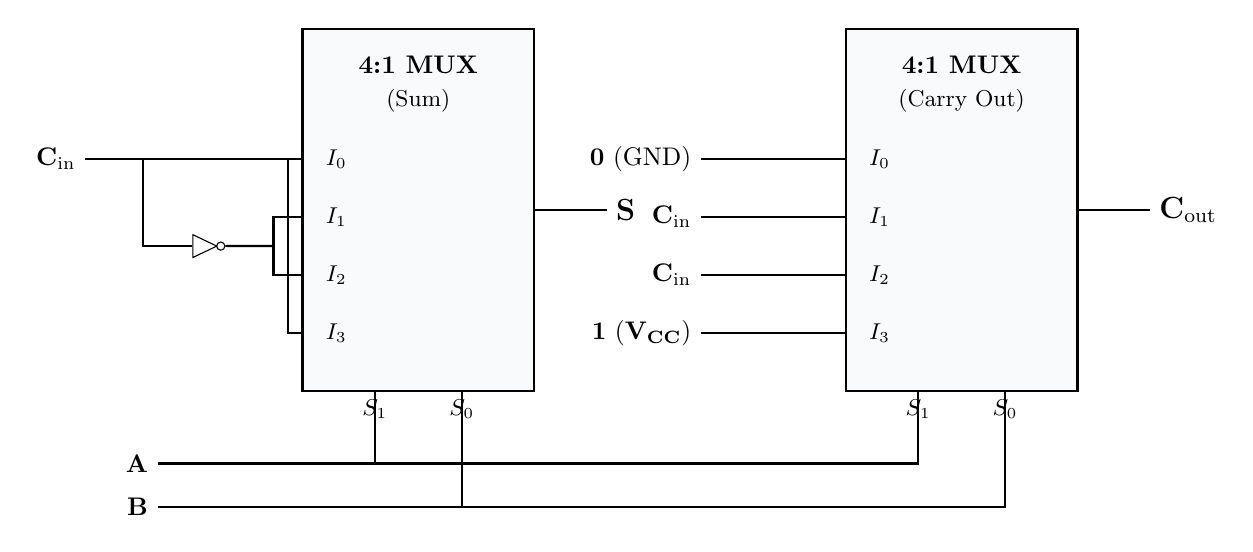
\begin{tikzpicture}[scale=0.92, transform shape]
  % MUX 1: Sum
  \draw[thick, fill=boxbg] (0, 0) rectangle (3.2, 5.0);
  \node at (1.6, 4.5) {\textbf{4:1 MUX}};
  \node at (1.6, 4.0) {\small (Sum)};
  \node[anchor=west] at (0.2, 3.2) {\small $I_0$};
  \node[anchor=west] at (0.2, 2.4) {\small $I_1$};
  \node[anchor=west] at (0.2, 1.6) {\small $I_2$};
  \node[anchor=west] at (0.2, 0.8) {\small $I_3$};
  \node[anchor=north] at (1.0, 0) {\small $S_1$};
  \node[anchor=north] at (2.2, 0) {\small $S_0$};
  \draw[thick] (3.2, 2.5) -- ++(1.0, 0) node[right] {\large $\mathbf{S}$};

  % MUX 2: Carry Out
  \draw[thick, fill=boxbg] (7.5, 0) rectangle (10.7, 5.0);
  \node at (9.1, 4.5) {\textbf{4:1 MUX}};
  \node at (9.1, 4.0) {\small (Carry Out)};
  \node[anchor=west] at (7.7, 3.2) {\small $I_0$};
  \node[anchor=west] at (7.7, 2.4) {\small $I_1$};
  \node[anchor=west] at (7.7, 1.6) {\small $I_2$};
  \node[anchor=west] at (7.7, 0.8) {\small $I_3$};
  \node[anchor=north] at (8.5, 0) {\small $S_1$};
  \node[anchor=north] at (9.7, 0) {\small $S_0$};
  \draw[thick] (10.7, 2.5) -- ++(1.0, 0) node[right] {\large $\mathbf{C_{\text{out}}}$};

  % Input Rails on Left
  \draw[thick] (-3.0, 3.2) -- (-2.2, 3.2) node[left, at start] {$\mathbf{C_{\text{in}}}$};
  \node[not gate US, draw, scale=0.8] (not1) at (-1.4, 2.0) {};
  \draw[thick] (-2.2, 3.2) -- (-0.2, 3.2) -- (0, 3.2);
  \draw[thick] (-2.2, 3.2) |- (not1.input);
  \draw[thick] (not1.output) -- (-0.4, 2.0);
  \draw[thick] (-0.4, 2.0) |- (0, 2.4);
  \draw[thick] (-0.4, 2.0) |- (0, 1.6);
  \draw[thick] (-0.2, 3.2) |- (0, 0.8);

  % MUX 2 inputs
  \draw[thick] (5.5, 3.2) node[left] {$\mathbf{0\ (\text{GND})}$} -- (7.5, 3.2);
  \draw[thick] (5.5, 2.4) node[left] {$\mathbf{C_{\text{in}}}$} -- (7.5, 2.4);
  \draw[thick] (5.5, 1.6) node[left] {$\mathbf{C_{\text{in}}}$} -- (7.5, 1.6);
  \draw[thick] (5.5, 0.8) node[left] {$\mathbf{1\ (V_{CC})}$} -- (7.5, 0.8);

  % Common Select lines A, B
  \draw[thick] (-2.0, -1.0) node[left] {$\mathbf{A}$} -- (1.0, -1.0) -- (1.0, 0);
  \draw[thick] (1.0, -1.0) -- (8.5, -1.0) -- (8.5, 0);
  \draw[thick] (-2.0, -1.6) node[left] {$\mathbf{B}$} -- (2.2, -1.6) -- (2.2, 0);
  \draw[thick] (2.2, -1.6) -- (9.7, -1.6) -- (9.7, 0);
\end{tikzpicture}
\end{schematicbox}

\begin{answerbox}
\textbf{Sum ($S$):} $I_0 = C_{\text{in}}, I_1 = \bar{C}_{\text{in}}, I_2 = \bar{C}_{\text{in}}, I_3 = C_{\text{in}}$.\\
\textbf{Carry Out ($C_{\text{out}}$):} $I_0 = 0, I_1 = C_{\text{in}}, I_2 = C_{\text{in}}, I_3 = 1$, with select lines $S_1 = A, S_0 = B$.
\end{answerbox}

\vspace{0.6cm}

% =========================================================================
% QUESTION 7
% =========================================================================
\subsection{Question 7: SR to JK Flip-Flop Conversion Schematic [2 + 5 = 7 Marks]}
\begin{questionbox}{Problem Statement (2082 Bhadra, Q7)}
Differentiate between combinational circuit and sequential circuit. With necessary steps and implementation, convert an SR flip-flop into a JK flip-flop.
\end{questionbox}

\paragraph{Part (a): Combinational vs. Sequential Circuits [2 Marks]}
\begin{center}
\small
\begin{tabular}{@{}p{3.2cm}p{6.8cm}p{6.8cm}@{}}
\toprule
\textbf{Parameter} & \textbf{Combinational Circuit} & \textbf{Sequential Circuit} \\
\midrule
\textbf{Output Dependence} & Depends strictly on the present inputs at that instant. & Depends on both present inputs and the past history (internal stored state). \\
\textbf{Memory Elements} & Contains no memory elements or feedback paths. & Contains memory elements (flip-flops, latches) with feedback loops. \\
\textbf{Clock Synchronization} & Clock signal is not required; operates asynchronously. & Usually driven by a synchronous master clock signal. \\
\textbf{Design Complexity} & Simple (Boolean algebraic minimization, K-maps). & Complex (State tables, state diagrams, FSM models). \\
\textbf{Examples} & Adders, Subtractors, Multiplexers, Decoders. & Flip-flops, Counters, Shift registers, CPUs. \\
\bottomrule
\end{tabular}
\end{center}

\paragraph{Part (b): Conversion of SR Flip-Flop into JK Flip-Flop [5 Marks]}
\begin{enumerate}
  \item \textbf{Target:} JK Flip-Flop with inputs $J, K$, present state $Q_n$, next state $Q_{n+1}$.
  \item \textbf{Available:} SR Flip-Flop with excitation requirements:
  \[
  \begin{array}{cc|cc}
  Q_n & Q_{n+1} & S & R \\ \hline
  0 & 0 & 0 & X \\
  0 & 1 & 1 & 0 \\
  1 & 0 & 0 & 1 \\
  1 & 1 & X & 0
  \end{array}
  \]
\end{enumerate}

\paragraph{Conversion Table:}
\begin{center}
\begin{tabular}{|ccc||c||cc|}
\hline
$\mathbf{J}$ & $\mathbf{K}$ & $\mathbf{Q_n}$ & $\mathbf{Q_{n+1}}$ & $\mathbf{S}$ & $\mathbf{R}$ \\ \hline
0 & 0 & 0 & 0 & 0 & $X$ \\ \hline
0 & 0 & 1 & 1 & $X$ & 0 \\ \hline
0 & 1 & 0 & 0 & 0 & $X$ \\ \hline
0 & 1 & 1 & 0 & 0 & 1 \\ \hline
1 & 0 & 0 & 1 & 1 & 0 \\ \hline
1 & 0 & 1 & 1 & $X$ & 0 \\ \hline
1 & 1 & 0 & 1 & 1 & 0 \\ \hline
1 & 1 & 1 & 0 & 0 & 1 \\ \hline
\end{tabular}
\end{center}

\paragraph{K-Map Minimization for $S$ and $R$:}
\begin{itemize}
  \item For $S(J, K, Q_n)$: Minterms are $m_4, m_6$; Don't cares are $d_1, d_5 \implies \mathbf{S = J\bar{Q}_n}$.
  \item For $R(J, K, Q_n)$: Minterms are $m_3, m_7$; Don't cares are $d_0, d_2 \implies \mathbf{R = KQ_n}$.
\end{itemize}

\begin{schematicbox}{SR Flip-Flop Converted to JK Flip-Flop}
\centering
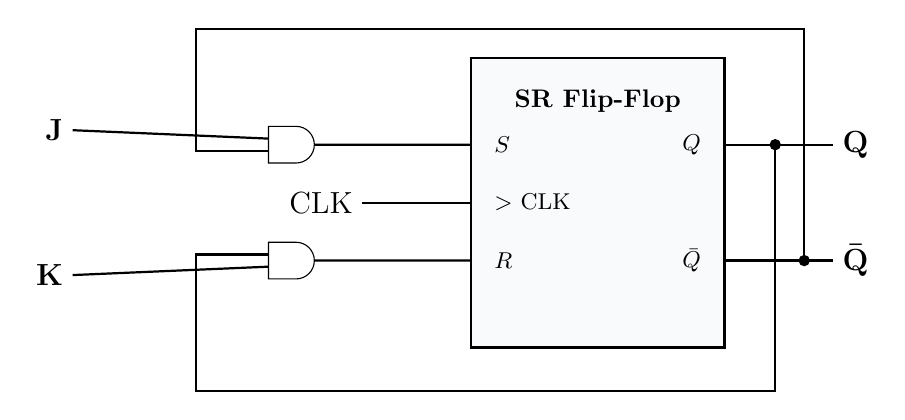
\begin{tikzpicture}[scale=0.92, transform shape]
  % SR Flip Flop Box
  \draw[thick, fill=boxbg] (7.0, 0) rectangle (10.5, 4.0);
  \node at (8.75, 3.4) {\textbf{SR Flip-Flop}};
  \node[anchor=west] at (7.2, 2.8) {\small $S$};
  \node[anchor=west] at (7.2, 2.0) {\small $>$ \text{CLK}};
  \node[anchor=west] at (7.2, 1.2) {\small $R$};
  \node[anchor=east] at (10.3, 2.8) {\small $Q$};
  \node[anchor=east] at (10.3, 1.2) {\small $\bar{Q}$};

  % Clock line
  \draw[thick] (5.5, 2.0) -- (7.0, 2.0) node[left, at start] {\large $\mathbf{\text{CLK}}$};

  % AND gates on Left
  \node[and gate US, draw, logic gate inputs=nn] (andS) at (4.5, 2.8) {};
  \node[and gate US, draw, logic gate inputs=nn] (andR) at (4.5, 1.2) {};

  \draw[thick] (andS.output) -- (7.0, 2.8);
  \draw[thick] (andR.output) -- (7.0, 1.2);

  % Inputs J and K
  \draw[thick] (1.5, 3.0) node[left] {\large $\mathbf{J}$} -- (andS.input 1);
  \draw[thick] (1.5, 1.0) node[left] {\large $\mathbf{K}$} -- (andR.input 2);

  % Outputs Q and Q_bar
  \draw[thick] (10.5, 2.8) -- ++(1.5, 0) node[right] {\large $\mathbf{Q}$};
  \draw[thick] (10.5, 1.2) -- ++(1.5, 0) node[right] {\large $\mathbf{\bar{Q}}$};

  % Feedback Q to andR.input 1
  \filldraw[black] (11.2, 2.8) circle (2pt);
  \draw[thick] (11.2, 2.8) -- (11.2, -0.6) -- (3.2, -0.6) |- (andR.input 1);

  % Feedback Q_bar to andS.input 2
  \filldraw[black] (11.6, 1.2) circle (2pt);
  \draw[thick] (11.6, 1.2) -- (11.6, 4.4) -- (3.2, 4.4) |- (andS.input 2);
\end{tikzpicture}
\end{schematicbox}

\begin{answerbox}
$$\mathbf{S = J\bar{Q}, \qquad R = KQ}$$
An SR flip-flop is converted into a JK flip-flop by connecting $S = J\bar{Q}$ and $R = KQ$. This eliminates the invalid state ($S=R=1$) and enables toggling ($J=K=1$).
\end{answerbox}

\vspace{0.6cm}

% =========================================================================
% QUESTION 8
% =========================================================================
\subsection{Question 8: Types of Shift Registers \& 4-Bit Johnson Counter [2 + 3 = 5 Marks]}
\begin{questionbox}{Problem Statement (2082 Bhadra, Q8)}
Write briefly about different types of shift registers. With necessary circuit and timing diagrams, explain the operation of how the shift register is used as a Johnson's Counter.
\end{questionbox}

\paragraph{Part (a): Classification of Shift Registers [2 Marks]}
\begin{enumerate}
  \item \textbf{SISO (Serial-In Serial-Out):} Data loaded and retrieved serially. Used for time delay generation.
  \item \textbf{SIPO (Serial-In Parallel-Out):} Data loaded serially and read out in parallel. Used for serial-to-parallel data conversion.
  \item \textbf{PISO (Parallel-In Serial-Out):} Data loaded simultaneously in parallel and shifted out serially. Used in serial transmitters (e.g. UART).
  \item \textbf{PIPO (Parallel-In Parallel-Out):} Data loaded and read out simultaneously. Used as general-purpose internal CPU registers.
  \item \textbf{Bidirectional / Universal Shift Register:} Can shift data left, right, load parallel data, or hold state based on mode select lines.
\end{enumerate}

\paragraph{Part (b): 4-Bit Johnson (Twisted Ring) Counter [3 Marks]}
A \textbf{Johnson Counter} (or Moebius Counter) is constructed from an $n$-bit shift register by connecting the inverted output of the last stage ($\bar{Q}_3$) back to the data input of the first stage ($D_0$):
\[
D_0 = \bar{Q}_3
\]
An $n$-bit Johnson counter yields $2n$ unique states ($2 \times 4 = 8$ states for a 4-bit register), compared to $n$ states for a standard ring counter.

\begin{schematicbox}{4-Bit Johnson (Twisted-Ring) Counter Circuit Schematic}
\centering
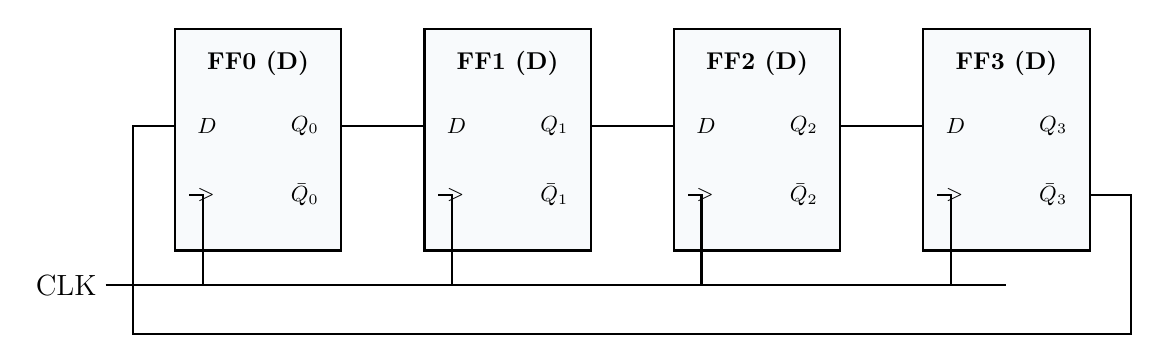
\begin{tikzpicture}[scale=0.88, transform shape]
  % 4 D Flip Flops
  \foreach \i in {0,1,2,3} {
    \draw[thick, fill=boxbg] ({3.6*\i}, 0) rectangle ({3.6*\i + 2.4}, 3.2);
    \node at ({3.6*\i + 1.2}, 2.7) {\textbf{FF\i\ (D)}};
    \node[anchor=west] at ({3.6*\i + 0.2}, 1.8) {\small $D$};
    \node[anchor=west] at ({3.6*\i + 0.2}, 0.8) {\small $>$};
    \node[anchor=east] at ({3.6*\i + 2.2}, 1.8) {\small $Q_\i$};
    \node[anchor=east] at ({3.6*\i + 2.2}, 0.8) {\small $\bar{Q}_\i$};
  }

  % Forward Shift Connections
  \draw[thick] (2.4, 1.8) -- (3.6, 1.8);
  \draw[thick] (6.0, 1.8) -- (7.2, 1.8);
  \draw[thick] (9.6, 1.8) -- (10.8, 1.8);

  % Inverted Feedback from FF3 Q_bar to FF0 D
  \draw[thick] (13.2, 0.8) -- (13.8, 0.8) -- (13.8, -1.2) -- (-0.6, -1.2) |- (0, 1.8);

  % Common Synchronous Clock
  \draw[thick] (-1.0, -0.5) node[left] {\large $\mathbf{\text{CLK}}$} -- (12.0, -0.5);
  \foreach \i in {0,1,2,3} {
    \draw[thick] ({3.6*\i + 0.4}, -0.5) -- ({3.6*\i + 0.4}, 0.8) -- ({3.6*\i + 0.2}, 0.8);
  }
\end{tikzpicture}
\end{schematicbox}

\paragraph{State Sequence Table (8 Distinct States):}
\begin{center}
\begin{tabular}{|c|cccc|l|}
\hline
\textbf{Clock Pulse} & $\mathbf{Q_0}$ & $\mathbf{Q_1}$ & $\mathbf{Q_2}$ & $\mathbf{Q_3}$ & \textbf{Next Input $D_0 = \bar{Q}_3$} \\ \hline
0 (Initial) & 0 & 0 & 0 & 0 & $D_0 = \bar{0} = 1$ \\ \hline
1 & 1 & 0 & 0 & 0 & $D_0 = \bar{0} = 1$ \\ \hline
2 & 1 & 1 & 0 & 0 & $D_0 = \bar{0} = 1$ \\ \hline
3 & 1 & 1 & 1 & 0 & $D_0 = \bar{0} = 1$ \\ \hline
4 & 1 & 1 & 1 & 1 & $D_0 = \bar{1} = 0$ \\ \hline
5 & 0 & 1 & 1 & 1 & $D_0 = \bar{1} = 0$ \\ \hline
6 & 0 & 0 & 1 & 1 & $D_0 = \bar{1} = 0$ \\ \hline
7 & 0 & 0 & 0 & 1 & $D_0 = \bar{1} = 0$ \\ \hline
8 (Recycles) & 0 & 0 & 0 & 0 & Recycles to state 0 \\ \hline
\end{tabular}
\end{center}

\begin{answerbox}
A 4-bit Johnson counter provides $\mathbf{2n = 8}$ decoding states with adjacent states differing by only a single bit (Gray-code property), operating as a divide-by-8 frequency scaler.
\end{answerbox}

\vspace{0.6cm}

% =========================================================================
% QUESTION 9
% =========================================================================
\subsection{Question 9: 3-Bit Ripple UP Counter with Positive Edge Triggering [5 Marks]}
\begin{questionbox}{Problem Statement (2082 Bhadra, Q9)}
Describe the operation of 3-bit ripple up counter with positive edge triggered clock.
\end{questionbox}

A \textbf{3-Bit Ripple UP Counter} counts through 8 binary states from $000_2$ to $111_2$. 

\paragraph{Clocking Principle for Positive-Edge Triggered Flip-Flops:}
\begin{itemize}
  \item In a ripple UP counter, the next higher bit $Q_{i+1}$ must toggle whenever the current bit $Q_i$ transitions from $\mathbf{1 \to 0}$.
  \item Since the flip-flops are \textbf{positive edge-triggered} ($\uparrow$, triggering on $0 \to 1$), the transition $Q_i: 1 \to 0$ corresponds to inverted output $\bar{Q}_i: 0 \to 1$.
  \item Therefore, to achieve UP counting with positive-edge triggered flip-flops, the clock input of each subsequent flip-flop must be driven by the \textbf{complementary output $\bar{Q}$} of the preceding stage:
  \[
  \text{CLK}_{i+1} = \bar{Q}_i
  \]
\end{itemize}

\begin{schematicbox}{3-Bit Positive-Edge Triggered Ripple UP Counter}
\centering
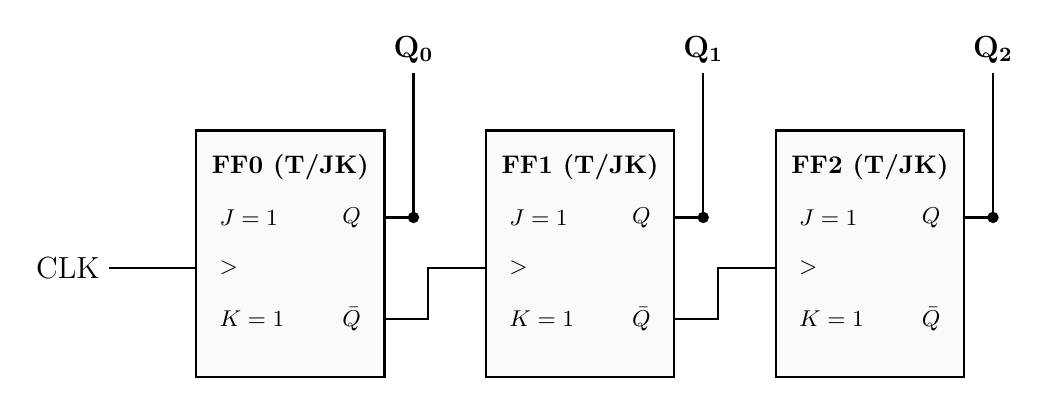
\begin{tikzpicture}[scale=0.92, transform shape]
  % 3 JK Flip Flops
  \foreach \i in {0,1,2} {
    \draw[thick, fill=boxbg] ({4.0*\i}, 0) rectangle ({4.0*\i + 2.6}, 3.4);
    \node at ({4.0*\i + 1.3}, 2.9) {\textbf{FF\i\ (T/JK)}};
    \node[anchor=west] at ({4.0*\i + 0.2}, 2.2) {\small $J=1$};
    \node[anchor=west] at ({4.0*\i + 0.2}, 1.5) {\small $>$};
    \node[anchor=west] at ({4.0*\i + 0.2}, 0.8) {\small $K=1$};
    \node[anchor=east] at ({4.0*\i + 2.4}, 2.2) {\small $Q$};
    \node[anchor=east] at ({4.0*\i + 2.4}, 0.8) {\small $\bar{Q}$};

    % Output pins
    \filldraw[black] ({4.0*\i + 3.0}, 2.2) circle (2pt);
    \draw[thick] ({4.0*\i + 2.6}, 2.2) -- ({4.0*\i + 3.0}, 2.2) -- ({4.0*\i + 3.0}, 4.2) node[above] {\large $\mathbf{Q_\i}$};
  }

  % External Clock to FF0
  \draw[thick] (-1.2, 1.5) node[left] {\large $\mathbf{\text{CLK}}$} -- (0, 1.5);

  % Ripple Connections: Q_bar_i -> CLK_{i+1}
  \draw[thick] (2.6, 0.8) -- (3.2, 0.8) |- (4.0, 1.5);
  \draw[thick] (6.6, 0.8) -- (7.2, 0.8) |- (8.0, 1.5);
\end{tikzpicture}
\end{schematicbox}

\begin{answerbox}
By connecting $\text{CLK}_{i+1} = \bar{Q}_i$, the positive-edge triggered flip-flops toggle on every $1 \to 0$ transition of $Q_i$, producing the standard binary UP counting sequence: $\mathbf{000 \to 001 \to 010 \to 011 \to 100 \to 101 \to 110 \to 111 \to 000}$.
\end{answerbox}

\vspace{0.6cm}

% =========================================================================
% QUESTION 10
% =========================================================================
\subsection{Question 10: Synchronous Mod-6 Counter Using SR Flip-Flops [7 Marks]}
\begin{questionbox}{Problem Statement (2082 Bhadra, Q10)}
Design the synchronous mod-6 counter using S-R flip-flop and draw its timing diagram also.
\end{questionbox}

A \textbf{Synchronous Mod-6 Counter} counts through 6 states: $000 \to 001 \to 010 \to 011 \to 100 \to 101 \to 000$. Requires $N = 3$ flip-flops ($2^2 < 6 \le 2^3$). Unused states: $110, 111$ (Don't Cares).

\paragraph{1. State Transition and SR Excitation Table:}
\begin{center}
\begin{tabular}{|c|ccc|ccc|cccccc|}
\hline
\textbf{State} & \multicolumn{3}{c|}{\textbf{Present State}} & \multicolumn{3}{c|}{\textbf{Next State}} & \multicolumn{6}{c|}{\textbf{SR Flip-Flop Inputs}} \\
& $Q_2$ & $Q_1$ & $Q_0$ & $Q_2^+$ & $Q_1^+$ & $Q_0^+$ & $\mathbf{S_2}$ & $\mathbf{R_2}$ & $\mathbf{S_1}$ & $\mathbf{R_1}$ & $\mathbf{S_0}$ & $\mathbf{R_0}$ \\ \hline
0 & 0 & 0 & 0 & 0 & 0 & 1 & 0 & $X$ & 0 & $X$ & 1 & 0 \\ \hline
1 & 0 & 0 & 1 & 0 & 1 & 0 & 0 & $X$ & 1 & 0 & 0 & 1 \\ \hline
2 & 0 & 1 & 0 & 0 & 1 & 1 & 0 & $X$ & $X$ & 0 & 1 & 0 \\ \hline
3 & 0 & 1 & 1 & 1 & 0 & 0 & 1 & 0 & 0 & 1 & 0 & 1 \\ \hline
4 & 1 & 0 & 0 & 1 & 0 & 1 & $X$ & 0 & 0 & $X$ & 1 & 0 \\ \hline
5 & 1 & 0 & 1 & 0 & 0 & 0 & 0 & 1 & 0 & $X$ & 0 & 1 \\ \hline
\end{tabular}
\end{center}

\paragraph{2. Minimized Equations via K-Maps:}
\begin{align*}
S_0 &= \bar{Q}_0, \qquad R_0 = Q_0 \\
S_1 &= \bar{Q}_2 \bar{Q}_1 Q_0, \qquad R_1 = Q_1 Q_0 \\
S_2 &= Q_1 Q_0, \qquad R_2 = Q_2 Q_0
\end{align*}

\paragraph{3. Self-Starting \& Lock-out Verification:}
\begin{itemize}
  \item If in state $110_2$: $S_0=1, R_0=0 \implies Q_0^+=1$; $S_1=0, R_1=0 \implies Q_1^+=1$; $S_2=0, R_2=0 \implies Q_2^+=1 \implies \text{Next State } 111_2$.
  \item If in state $111_2$: $S_0=0, R_0=1 \implies Q_0^+=0$; $S_1=0, R_1=1 \implies Q_1^+=0$; $S_2=0, R_2=1 \implies Q_2^+=0 \implies \text{Next State } 000_2$ (Valid state!).
\end{itemize}
Thus, the counter is completely self-starting and cannot get trapped in unused states.

\begin{schematicbox}{Synchronous Mod-6 Counter Logic Circuit Using SR Flip-Flops}
\centering
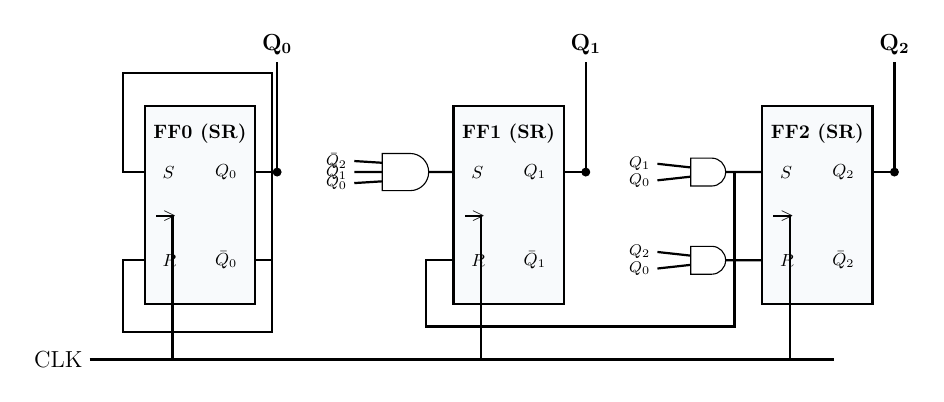
\begin{tikzpicture}[scale=0.70, transform shape]
  % 3 SR Flip Flops (Width 2.0 each, wide 3.6cm inter-stage gaps)
  % FF0: x in [0, 2.0]
  % FF1: x in [5.6, 7.6]
  % FF2: x in [11.2, 13.2]
  \foreach \i/\xpos in {0/0, 1/5.6, 2/11.2} {
    \draw[thick, fill=boxbg] (\xpos, 0) rectangle (\xpos + 2.0, 3.6);
    \node at (\xpos + 1.0, 3.1) {\textbf{FF\i\ (SR)}};
    \node[anchor=west] at (\xpos + 0.2, 2.4) {\small $S$};
    \node[anchor=west] at (\xpos + 0.2, 1.6) {\small $>$};
    \node[anchor=west] at (\xpos + 0.2, 0.8) {\small $R$};
    \node[anchor=east] at (\xpos + 1.8, 2.4) {\small $Q_\i$};
    \node[anchor=east] at (\xpos + 1.8, 0.8) {\small $\bar{Q}_\i$};

    \filldraw[black] (\xpos + 2.4, 2.4) circle (2pt);
    \draw[thick] (\xpos + 2.0, 2.4) -- (\xpos + 2.4, 2.4) -- (\xpos + 2.4, 4.4) node[above] {\large $\mathbf{Q_\i}$};
  }

  % Common Synchronous Clock
  \draw[thick] (-1.0, -1.0) node[left] {\large $\mathbf{\text{CLK}}$} -- (12.5, -1.0);
  \foreach \xpos in {0, 5.6, 11.2} {
    \draw[thick] (\xpos + 0.5, -1.0) -- (\xpos + 0.5, 1.6) -- (\xpos + 0.2, 1.6);
  }

  % FF0 Connections: S0 = Q0_bar (over top), R0 = Q0 (under bottom)
  \draw[thick] (2.0, 0.8) -- (2.3, 0.8) -- (2.3, 4.2) -- (-0.4, 4.2) |- (0, 2.4); % S0 = Q0_bar
  \draw[thick] (2.0, 2.4) -- (2.3, 2.4) -- (2.3, -0.5) -- (-0.4, -0.5) |- (0, 0.8); % R0 = Q0

  % Logic for S1 = Q2_bar . Q1_bar . Q0 (centered in gap [2.3, 5.6])
  \node[and gate US, draw, logic gate inputs=nnn] (andS1) at (4.7, 2.4) {};
  \draw[thick] (3.8, 2.6) node[left] {\footnotesize $\bar{Q}_2$} -- (andS1.input 1);
  \draw[thick] (3.8, 2.4) node[left] {\footnotesize $\bar{Q}_1$} -- (andS1.input 2);
  \draw[thick] (3.8, 2.2) node[left] {\footnotesize $Q_0$} -- (andS1.input 3);
  \draw[thick] (andS1.output) -- (5.6, 2.4);

  % AND Gate for S2 = Q1.Q0 and R1 = Q1.Q0 (in gap [7.6, 11.2])
  \node[and gate US, draw, logic gate inputs=nn] (andQ1Q0) at (10.2, 2.4) {};
  \draw[thick] (9.3, 2.55) node[left] {\footnotesize $Q_1$} -- (andQ1Q0.input 1);
  \draw[thick] (9.3, 2.25) node[left] {\footnotesize $Q_0$} -- (andQ1Q0.input 2);
  \draw[thick] (andQ1Q0.output) -- (11.2, 2.4); % S2
  \draw[thick] (10.7, 2.4) -- (10.7, -0.4) -- (5.1, -0.4) |- (5.6, 0.8); % R1

  % Logic for R2 = Q2 . Q0 (in gap [7.6, 11.2])
  \node[and gate US, draw, logic gate inputs=nn] (andR2) at (10.2, 0.8) {};
  \draw[thick] (9.3, 0.95) node[left] {\footnotesize $Q_2$} -- (andR2.input 1);
  \draw[thick] (9.3, 0.65) node[left] {\footnotesize $Q_0$} -- (andR2.input 2);
  \draw[thick] (andR2.output) -- (11.2, 0.8);
\end{tikzpicture}
\end{schematicbox}

\begin{answerbox}
$$\mathbf{S_0 = \bar{Q}_0, \ R_0 = Q_0, \quad S_1 = \bar{Q}_2 \bar{Q}_1 Q_0, \ R_1 = Q_1 Q_0, \quad S_2 = Q_1 Q_0, \ R_2 = Q_2 Q_0}$$
\end{answerbox}

\vspace{0.6cm}

% =========================================================================
% QUESTION 11
% =========================================================================
\subsection{Question 11: Synchronous FSM Sequence Detector '110' [7 Marks]}
\begin{questionbox}{Problem Statement (2082 Bhadra, Q11)}
Design a synchronous sequential machine that has 1-bit serial input $X$ and output $Z$ which will be high when the input contains the message `110' (Use SR Flip-Flop).
\end{questionbox}

\paragraph{1. State Definitions (Mealy Model):}
\begin{itemize}
  \item $S_0 (00)$: Reset state / No relevant bit detected.
  \item $S_1 (01)$: Pattern `1' detected.
  \item $S_2 (10)$: Pattern `11' detected.
  \item When in $S_2$ and $X=0 \implies$ `110' detected $\implies Z=1$, next state $S_0$.
\end{itemize}

\begin{schematicbox}{State Diagram for '110' Sequence Detector}
\centering
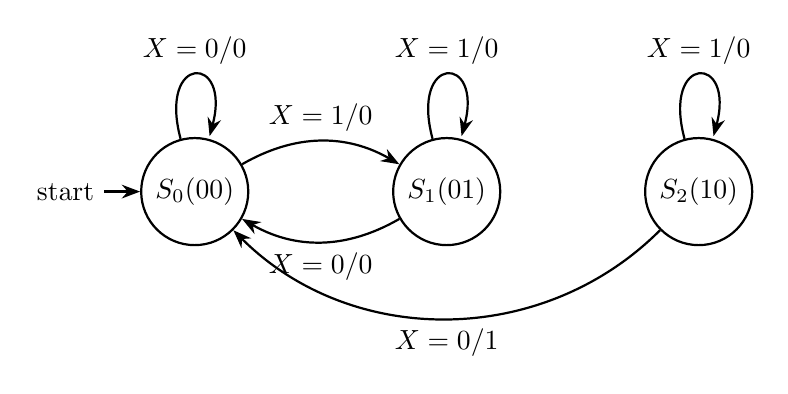
\begin{tikzpicture}[->, >=Stealth, auto, node distance=3.2cm, thick]
  \node[state, initial] (S0) {$S_0 (00)$};
  \node[state] (S1) [right of=S0] {$S_1 (01)$};
  \node[state] (S2) [right of=S1] {$S_2 (10)$};

  \path (S0) edge [loop above] node {$X=0 / 0$} (S0)
             edge [bend left] node {$X=1 / 0$} (S1)
        (S1) edge [loop above] node {$X=1 / 0$} (S2)
             edge [bend left] node {$X=0 / 0$} (S0)
        (S2) edge [loop above] node {$X=1 / 0$} (S2)
             edge [bend left=45] node {$X=0 / 1$} (S0);
\end{tikzpicture}
\end{schematicbox}

\paragraph{2. State Transition \& SR Excitation Table (Flip-Flops $A, B$):}
\begin{center}
\begin{tabular}{|cc|c|cc|c|cccc|}
\hline
\multicolumn{2}{|c|}{\textbf{Present State}} & \textbf{Input} & \multicolumn{2}{c|}{\textbf{Next State}} & \textbf{Output} & \multicolumn{4}{c|}{\textbf{SR Inputs}} \\
$A$ & $B$ & $X$ & $A^+$ & $B^+$ & $\mathbf{Z}$ & $\mathbf{S_A}$ & $\mathbf{R_A}$ & $\mathbf{S_B}$ & $\mathbf{R_B}$ \\ \hline
0 & 0 & 0 & 0 & 0 & 0 & 0 & $X$ & 0 & $X$ \\ \hline
0 & 0 & 1 & 0 & 1 & 0 & 0 & $X$ & 1 & 0 \\ \hline
0 & 1 & 0 & 0 & 0 & 0 & 0 & $X$ & 0 & 1 \\ \hline
0 & 1 & 1 & 1 & 0 & 0 & 1 & 0 & 0 & 1 \\ \hline
1 & 0 & 0 & 0 & 0 & 1 & 0 & 1 & 0 & $X$ \\ \hline
1 & 0 & 1 & 1 & 0 & 0 & $X$ & 0 & 0 & $X$ \\ \hline
1 & 1 & 0 & $X$ & $X$ & $X$ & $X$ & $X$ & $X$ & $X$ \\ \hline
1 & 1 & 1 & $X$ & $X$ & $X$ & $X$ & $X$ & $X$ & $X$ \\ \hline
\end{tabular}
\end{center}

\paragraph{3. Minimized Equations via K-Maps:}
\begin{align*}
S_A &= BX, \qquad R_A = \bar{X} \\
S_B &= \bar{A}\bar{B}X, \qquad R_B = \bar{X} + B \\
Z &= A\bar{X}
\end{align*}

\begin{answerbox}
$$\mathbf{S_A = BX, \quad R_A = \bar{X}, \quad S_B = \bar{A}\bar{B}X, \quad R_B = \bar{X} + B, \quad Z = A\bar{X}}$$
\end{answerbox}

\vspace{0.6cm}

% =========================================================================
% QUESTION 12
% =========================================================================
\subsection{Question 12: Frequency Counter Block Diagram [3 Marks]}
\begin{questionbox}{Problem Statement (2082 Bhadra, Q12)}
Write a short note on frequency counter.
\end{questionbox}

A \textbf{Digital Frequency Counter} is an electronic test instrument that accurately measures the frequency of an unknown periodic input signal by counting the number of cycles ($N$) that occur during a precisely controlled time window ($T_{\text{gate}}$):
\[
f_x = \frac{N}{T_{\text{gate}}}
\]

\paragraph{Core Functional Subsystems:}
\begin{enumerate}
  \item \textbf{Input Attenuator \& Amplifier:} Scales input voltage to safe operational levels.
  \item \textbf{Schmitt Trigger (Wave Shaper):} Converts arbitrary input waveforms (sinusoidal, triangular) into sharp, clean digital rectangular pulses.
  \item \textbf{Crystal Oscillator \& Time Base Generator:} Highly stable quartz crystal oscillator (e.g. 1 MHz or 10 MHz) paired with decade frequency dividers to produce accurate gate periods ($1\text{ ms}, 10\text{ ms}, 0.1\text{ s}, 1\text{ s}$).
  \item \textbf{Main Gate (AND Gate):} Enabled for exactly $T_{\text{gate}}$, passing $N$ input pulses to the counter.
  \item \textbf{Decade Counter, Latch, \& Display:} Counts incoming pulses, latches the result, and drives 7-segment digital displays.
\end{enumerate}

\begin{schematicbox}{Functional Block Diagram of a Digital Frequency Counter}
\centering
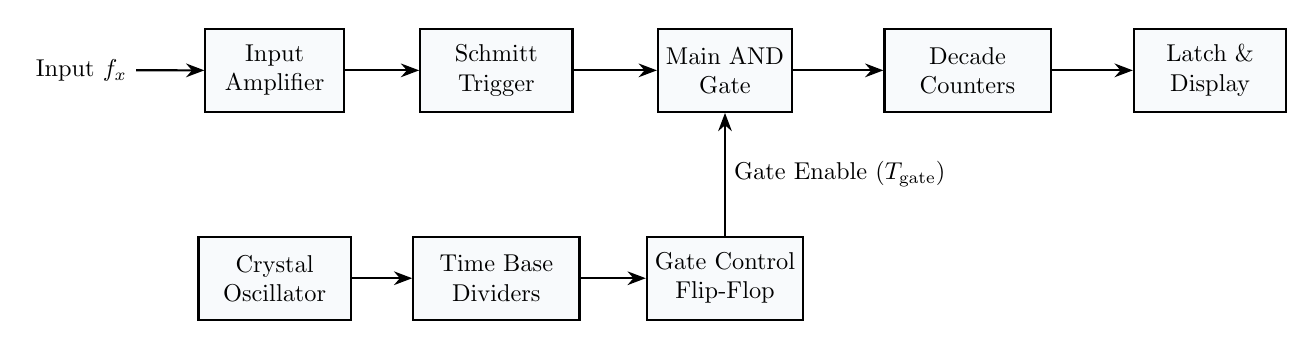
\begin{tikzpicture}[scale=0.88, transform shape, >=Stealth]
  % Input blocks
  \node[draw, thick, fill=boxbg, minimum width=2.0cm, minimum height=1.2cm, align=center] (amp) at (0, 3) {Input\\Amplifier};
  \node[draw, thick, fill=boxbg, minimum width=2.2cm, minimum height=1.2cm, align=center] (schmitt) at (3.2, 3) {Schmitt\\Trigger};
  \node[draw, thick, fill=boxbg, minimum width=1.6cm, minimum height=1.2cm, align=center] (gate) at (6.5, 3) {Main AND\\Gate};
  \node[draw, thick, fill=boxbg, minimum width=2.4cm, minimum height=1.2cm, align=center] (counter) at (10.0, 3) {Decade\\Counters};
  \node[draw, thick, fill=boxbg, minimum width=2.2cm, minimum height=1.2cm, align=center] (disp) at (13.5, 3) {Latch \&\\Display};

  \draw[thick, ->] (-2.0, 3) node[left] {Input $f_x$} -- (amp.west);
  \draw[thick, ->] (amp.east) -- (schmitt.west);
  \draw[thick, ->] (schmitt.east) -- (gate.west);
  \draw[thick, ->] (gate.east) -- (counter.west);
  \draw[thick, ->] (counter.east) -- (disp.west);

  % Time base blocks
  \node[draw, thick, fill=boxbg, minimum width=2.2cm, minimum height=1.2cm, align=center] (osc) at (0, 0) {Crystal\\Oscillator};
  \node[draw, thick, fill=boxbg, minimum width=2.4cm, minimum height=1.2cm, align=center] (div) at (3.2, 0) {Time Base\\Dividers};
  \node[draw, thick, fill=boxbg, minimum width=2.2cm, minimum height=1.2cm, align=center] (gctrl) at (6.5, 0) {Gate Control\\Flip-Flop};

  \draw[thick, ->] (osc.east) -- (div.west);
  \draw[thick, ->] (div.east) -- (gctrl.west);
  \draw[thick, ->] (gctrl.north) -- (gate.south) node[midway, right] {Gate Enable ($T_{\text{gate}}$)};
\end{tikzpicture}
\end{schematicbox}

\begin{answerbox}
A frequency counter counts incoming signal transitions over a precision gate window $T_{\text{gate}}$, calculating frequency via $\mathbf{f = N / T_{\text{gate}}}$.
\end{answerbox}

\chapter{2082 Baishakh Examination Solutions}

\section*{Examination Overview}
\begin{tabular}{@{}ll@{}}
\textbf{Level:} Bachelor in Engineering (BE) & \textbf{Full Marks:} 60 \\
\textbf{Programme:} BCT, BEI & \textbf{Pass Marks:} 24 \\
\textbf{Year / Part:} I / II & \textbf{Time:} 3 Hours \\
\textbf{Subject:} Digital Logic (EX 152) & \textbf{Examination Type:} Back (New Course) \\
\end{tabular}

\vspace{0.6cm}
\hrule
\vspace{0.6cm}

% =========================================================================
% QUESTION 1
% =========================================================================
\subsection{Question 1: ASCII Code \& 2's Complement Addition [1 + 3 = 4 Marks]}
\begin{questionbox}{Problem Statement (2082 Baishakh, Q1)}
Define an ASCII code. Use 2's complement method to perform the following addition $(-28 + 12)_{10}$ in 8-bit signed number representation.
\end{questionbox}

\paragraph{Part (a): Definition of ASCII Code [1 Mark]}
\textbf{ASCII} (\textit{American Standard Code for Information Interchange}) is a standardized alphanumeric character encoding scheme:
\begin{itemize}
  \item Standard ASCII uses a \textbf{7-bit binary code} to represent $2^7 = 128$ distinct characters, including English alphabets ($A-Z, a-z$), numerals ($0-9$), punctuation symbols, and non-printable control characters (e.g., CR, LF, ESC).
  \item Extended ASCII uses an \textbf{8-bit code} ($2^8 = 256$ characters) to accommodate graphical symbols and international characters.
\end{itemize}

\paragraph{Part (b): 2's Complement Addition of $(-28 + 12)_{10}$ in 8 Bits [3 Marks]}
\begin{enumerate}
  \item \textbf{Representation of $+12_{10}$ in 8-bit binary:}
  \[
  +12_{10} = \mathbf{0000\ 1100_2}
  \]
  \item \textbf{Representation of $-28_{10}$ in 8-bit 2's complement form:}
  \[
  +28_{10} = 0001\ 1100_2
  \]
  Take 1's complement: $\text{1's comp}(0001\ 1100) = 1110\ 0011_2$. \\
  Add 1:
  \[
  -28_{10} = 1110\ 0011 + 1 = \mathbf{1110\ 0100_2}
  \]
  \item \textbf{Perform 8-bit Binary Addition:}
  \[
  \begin{array}{r@{\quad}l}
    1110\ 0100 & (-28_{10}) \\
  +\ 0000\ 1100 & (+12_{10}) \\
  \hline
    \mathbf{1111\ 0000_2} & \text{(Result in 2's complement form)}
  \end{array}
  \]
  \item \textbf{Verification and Decimal Interpretation:}
  \begin{itemize}
    \item MSB $= 1 \implies$ Result is \textbf{negative}.
    \item Magnitude $= \text{2's complement of } 1111\ 0000_2 = (0000\ 1111)_2 + 1 = 0001\ 0000_2 = \mathbf{16_{10}}$.
    \item Therefore, result is $\mathbf{-16_{10}}$, which matches $-28 + 12 = -16$.
  \end{itemize}
\end{enumerate}

\begin{answerbox}
$$(-28 + 12)_{10} = \mathbf{(1111\ 0000)_2} = -16_{10}$$
\end{answerbox}

\vspace{0.6cm}

% =========================================================================
% QUESTION 2
% =========================================================================
\subsection{Question 2: Boolean Algebra Proofs [2 + 2 = 4 Marks]}
\begin{questionbox}{Problem Statement (2082 Baishakh, Q2)}
Prove the following Boolean identities algebraically:
\begin{enumerate}[label=(\alph*)]
  \item $AB + \bar{A}C + BC = AB + \bar{A}C$
  \item $AB + C(A \oplus B) = BC + A(B+C)$
\end{enumerate}
\end{questionbox}

\paragraph{Part (a): Consensus Theorem Proof [2 Marks]}
To prove: $AB + \bar{A}C + BC = AB + \bar{A}C$.
\begin{align*}
\text{LHS} &= AB + \bar{A}C + BC \\
&= AB + \bar{A}C + BC(1) && \text{(Identity Law: } X \cdot 1 = X\text{)} \\
&= AB + \bar{A}C + BC(A + \bar{A}) && \text{(Complementarity Law: } A + \bar{A} = 1\text{)} \\
&= AB + \bar{A}C + ABC + \bar{A}BC && \text{(Distributive Law)} \\
&= (AB + ABC) + (\bar{A}C + \bar{A}BC) && \text{(Associative \& Commutative Laws)} \\
&= AB(1 + C) + \bar{A}C(1 + B) && \text{(Distributive Law)} \\
&= AB(1) + \bar{A}C(1) && \text{(Dominance Law: } 1 + X = 1\text{)} \\
&= AB + \bar{A}C = \text{RHS} \quad \blacksquare
\end{align*}

\paragraph{Part (b): Identity Proof [2 Marks]}
To prove: $AB + C(A \oplus B) = BC + A(B+C)$.
\begin{align*}
\text{LHS} &= AB + C(A \oplus B) \\
&= AB + C(A\bar{B} + \bar{A}B) && \text{(Definition of XOR: } A \oplus B = A\bar{B} + \bar{A}B\text{)} \\
&= AB + A\bar{B}C + \bar{A}BC \\
&= AB(1 + C) + A\bar{B}C + \bar{A}BC && \text{(Since } AB = AB(1+C) = AB + ABC\text{)} \\
&= AB + ABC + A\bar{B}C + \bar{A}BC \\
&= AB + AC(B + \bar{B}) + BC(A + \bar{A}) \\
&= AB + AC(1) + BC(1) \\
&= AB + AC + BC
\end{align*}
Now expanding the Right Hand Side (RHS):
\begin{align*}
\text{RHS} &= BC + A(B + C) \\
&= BC + AB + AC \\
&= AB + AC + BC
\end{align*}
Since $\text{LHS} = \text{RHS} = AB + AC + BC$, the identity is proved. $\blacksquare$

\begin{answerbox}
Both Boolean identities are formally verified using fundamental axioms and laws of Boolean algebra.
\end{answerbox}

\vspace{0.6cm}

% =========================================================================
% QUESTION 3
% =========================================================================
\subsection{Question 3: Octal Priority Encoder Schematic [2 + 6 = 8 Marks]}
\begin{questionbox}{Problem Statement (2082 Baishakh, Q3)}
What is a decoder? Design an octal priority encoder with neat circuit diagram.
\end{questionbox}

\paragraph{Part (a): Definition of Decoder [2 Marks]}
A \textbf{decoder} is a combinational logic circuit with $n$ input lines and $2^n$ unique output lines. It decodes an $n$-bit binary code word by asserting exactly one output line HIGH (or active LOW) corresponding to the decimal equivalent of the input binary code.

\paragraph{Part (b): Design of Octal Priority Encoder (8-to-3) [6 Marks]}
An \textbf{Octal Priority Encoder} accepts 8 input lines $D_0, D_1, \dots, D_7$ where input $D_7$ has the highest priority and $D_0$ has the lowest priority. If multiple inputs are HIGH simultaneously, the output binary code $A_2 A_1 A_0$ reflects the highest-indexed active input. A \textbf{Valid Output} bit ($V$) indicates whether any input is active.

\paragraph{Truth Table:}
\begin{center}
\small
\begin{tabular}{|cccccccc||ccc|c|}
\hline
$D_7$ & $D_6$ & $D_5$ & $D_4$ & $D_3$ & $D_2$ & $D_1$ & $D_0$ & $\mathbf{A_2}$ & $\mathbf{A_1}$ & $\mathbf{A_0}$ & $\mathbf{V\ (Valid)}$ \\ \hline
0 & 0 & 0 & 0 & 0 & 0 & 0 & 0 & $X$ & $X$ & $X$ & 0 \\ \hline
0 & 0 & 0 & 0 & 0 & 0 & 0 & 1 & 0 & 0 & 0 & 1 \\ \hline
0 & 0 & 0 & 0 & 0 & 0 & 1 & $X$ & 0 & 0 & 1 & 1 \\ \hline
0 & 0 & 0 & 0 & 0 & 1 & $X$ & $X$ & 0 & 1 & 0 & 1 \\ \hline
0 & 0 & 0 & 0 & 1 & $X$ & $X$ & $X$ & 0 & 1 & 1 & 1 \\ \hline
0 & 0 & 0 & 1 & $X$ & $X$ & $X$ & $X$ & 1 & 0 & 0 & 1 \\ \hline
0 & 0 & 1 & $X$ & $X$ & $X$ & $X$ & $X$ & 1 & 0 & 1 & 1 \\ \hline
0 & 1 & $X$ & $X$ & $X$ & $X$ & $X$ & $X$ & 1 & 1 & 0 & 1 \\ \hline
1 & $X$ & $X$ & $X$ & $X$ & $X$ & $X$ & $X$ & 1 & 1 & 1 & 1 \\ \hline
\end{tabular}
\end{center}

\paragraph{Minimized Boolean Output Equations:}
\begin{align*}
A_2 &= D_4 + D_5 + D_6 + D_7 \\
A_1 &= D_6 + D_7 + \bar{D}_6 \bar{D}_5 (D_2 + D_3) = D_6 + D_7 + D_2 \bar{D}_4 \bar{D}_5 + D_3 \bar{D}_4 \bar{D}_5 \\
A_0 &= D_7 + D_5 \bar{D}_6 + D_3 \bar{D}_4 \bar{D}_6 + D_1 \bar{D}_2 \bar{D}_4 \bar{D}_6 \\
V &= D_0 + D_1 + D_2 + D_3 + D_4 + D_5 + D_6 + D_7
\end{align*}

\begin{schematicbox}{Octal (8-to-3) Priority Encoder Circuit Schematic}
\centering
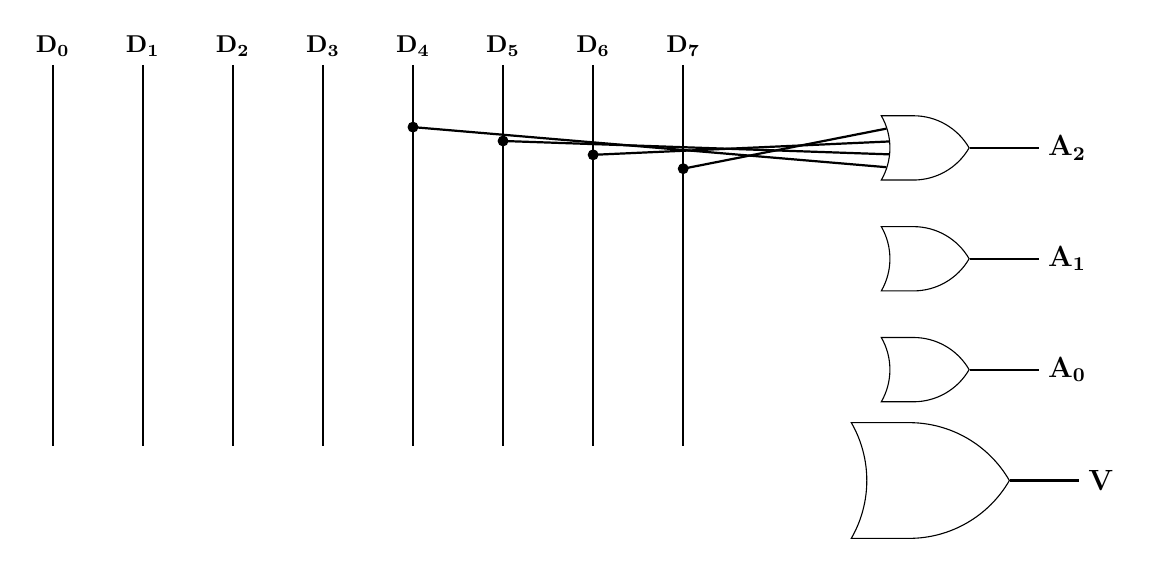
\begin{tikzpicture}[scale=0.88, transform shape]
  % Inputs vertical rails
  \foreach \i in {0,1,...,7} {
    \draw[thick] ({1.3*\i}, 6.0) -- ({1.3*\i}, 0.5);
    \node[above] at ({1.3*\i}, 6.0) {$\mathbf{D_\i}$};
  }

  % Output OR Gates
  \node[or gate US, draw, logic gate inputs=nnnn, scale=1.1] (orA2) at (12.5, 4.8) {};
  \node[or gate US, draw, logic gate inputs=nnnn, scale=1.1] (orA1) at (12.5, 3.2) {};
  \node[or gate US, draw, logic gate inputs=nnnn, scale=1.1] (orA0) at (12.5, 1.6) {};
  \node[or gate US, draw, logic gate inputs=nnnnnnnn, scale=1.1] (orV) at (12.5, 0.0) {};

  % Output lines
  \draw[thick] (orA2.output) -- ++(1.0, 0) node[right] {\large $\mathbf{A_2}$};
  \draw[thick] (orA1.output) -- ++(1.0, 0) node[right] {\large $\mathbf{A_1}$};
  \draw[thick] (orA0.output) -- ++(1.0, 0) node[right] {\large $\mathbf{A_0}$};
  \draw[thick] (orV.output) -- ++(1.0, 0) node[right] {\large $\mathbf{V}$};

  % Wire OR A2 (D4, D5, D6, D7)
  \filldraw[black] ({1.3*4}, 5.1) circle (2pt); \draw[thick] ({1.3*4}, 5.1) -- (orA2.input 4);
  \filldraw[black] ({1.3*5}, 4.9) circle (2pt); \draw[thick] ({1.3*5}, 4.9) -- (orA2.input 3);
  \filldraw[black] ({1.3*6}, 4.7) circle (2pt); \draw[thick] ({1.3*6}, 4.7) -- (orA2.input 2);
  \filldraw[black] ({1.3*7}, 4.5) circle (2pt); \draw[thick] ({1.3*7}, 4.5) -- (orA2.input 1);
\end{tikzpicture}
\end{schematicbox}

\begin{answerbox}
$$\mathbf{A_2 = D_4 + D_5 + D_6 + D_7, \quad A_1 = D_6 + D_7 + \bar{D}_4\bar{D}_5(D_2 + D_3), \quad V = \sum_{i=0}^7 D_i}$$
\end{answerbox}

\vspace{0.6cm}

% =========================================================================
% QUESTION 4
% =========================================================================
\subsection{Question 4: 3x8 Decoder Function Realization \& K-Map [3 + 3 = 6 Marks]}
\begin{questionbox}{Problem Statement (2082 Baishakh, Q4)}
Realize the Boolean function $X(A, B, C, D) = \sum m(0, 2, 3, 7, 8, 10, 11, 14, 15)$ using a single $3 \times 8$ decoder. Also simplify the logic function implementing K-map method.
\end{questionbox}

\paragraph{Part (a): Realization Using a Single $3 \times 8$ Decoder [3 Marks]}
Let variables $A, B, C$ be connected to decoder select inputs $S_2, S_1, S_0$, and let variable $D$ serve as external data input:
\begin{itemize}
  \item $Y_0 = \bar{A}\bar{B}\bar{C}$: includes $m_0(\bar{D}), m_1(D) \implies$ function has $m_0 \implies \mathbf{Y_0 \bar{D}}$.
  \item $Y_1 = \bar{A}\bar{B}C$: includes $m_2(\bar{D}), m_3(D) \implies$ function has both $m_2, m_3 \implies \mathbf{Y_1}$.
  \item $Y_2 = \bar{A}B\bar{C}$: includes $m_4, m_5 \implies 0$.
  \item $Y_3 = \bar{A}BC$: includes $m_6(\bar{D}), m_7(D) \implies$ function has $m_7 \implies \mathbf{Y_3 D}$.
  \item $Y_4 = A\bar{B}\bar{C}$: includes $m_8(\bar{D}), m_9(D) \implies$ function has $m_8 \implies \mathbf{Y_4 \bar{D}}$.
  \item $Y_5 = A\bar{B}C$: includes $m_{10}(\bar{D}), m_{11}(D) \implies$ function has both $m_{10}, m_{11} \implies \mathbf{Y_5}$.
  \item $Y_6 = AB\bar{C}$: includes $m_{12}, m_{13} \implies 0$.
  \item $Y_7 = ABC$: includes $m_{14}(\bar{D}), m_{15}(D) \implies$ function has both $m_{14}, m_{15} \implies \mathbf{Y_7}$.
\end{itemize}
Combining terms:
\[
X = (Y_0 + Y_4)\bar{D} + Y_1 + Y_3 D + Y_5 + Y_7
\]

\begin{schematicbox}{Function Realization Using Single 3x8 Decoder and Gates}
\centering
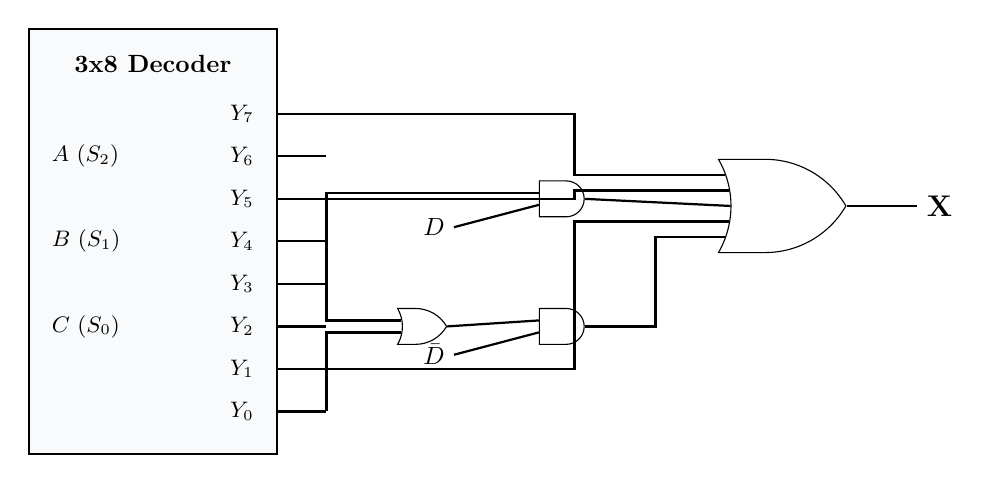
\begin{tikzpicture}[scale=0.9, transform shape]
  % 3x8 Decoder Box
  \draw[thick, fill=boxbg] (0, 0) rectangle (3.5, 6.0);
  \node at (1.75, 5.5) {\textbf{3x8 Decoder}};
  \node[anchor=west] at (0.2, 4.2) {\small $A\ (S_2)$};
  \node[anchor=west] at (0.2, 3.0) {\small $B\ (S_1)$};
  \node[anchor=west] at (0.2, 1.8) {\small $C\ (S_0)$};

  \foreach \i in {0,1,...,7} {
    \node[anchor=east] at (3.3, {0.6 + \i*0.6}) {\small $Y_\i$};
    \draw[thick] (3.5, {0.6 + \i*0.6}) -- (4.2, {0.6 + \i*0.6});
  }

  % Combinational Gates on right
  \node[or gate US, draw, logic gate inputs=nn] (or04) at (5.5, 1.8) {};
  \node[and gate US, draw, logic gate inputs=nn] (and04D) at (7.5, 1.8) {};
  \node[and gate US, draw, logic gate inputs=nn] (and3D) at (7.5, 3.6) {};

  % Final 5-input OR Gate
  \node[or gate US, draw, logic gate inputs=nnnnn, scale=1.3] (orOut) at (10.5, 3.5) {};

  % Connections
  \draw[thick] (4.2, 0.6) |- (or04.input 2); % Y0
  \draw[thick] (4.2, 3.0) |- (or04.input 1); % Y4
  \draw[thick] (or04.output) -- (and04D.input 1);
  \draw[thick] (6.0, 1.4) node[left] {$\bar{D}$} -- (and04D.input 2);

  \draw[thick] (4.2, 2.4) |- (and3D.input 1); % Y3
  \draw[thick] (6.0, 3.2) node[left] {$D$} -- (and3D.input 2);

  % Feeds into OR Out
  \draw[thick] (and04D.output) -- ++(1.0, 0) |- (orOut.input 5);
  \draw[thick] (4.2, 1.2) -- ++(3.5, 0) |- (orOut.input 4); % Y1
  \draw[thick] (and3D.output) -- (orOut.input 3);
  \draw[thick] (4.2, 3.6) -- ++(3.5, 0) |- (orOut.input 2); % Y5
  \draw[thick] (4.2, 4.8) -- ++(3.5, 0) |- (orOut.input 1); % Y7

  \draw[thick] (orOut.output) -- ++(1.0, 0) node[right] {\large $\mathbf{X}$};
\end{tikzpicture}
\end{schematicbox}

\paragraph{Part (b): K-Map Minimization [3 Marks]}
\begin{center}
\begin{tabular}{|c|c|c|c|c|}
\hline
$AB \ \backslash \ CD$ & \textbf{00} & \textbf{01} & \textbf{11} & \textbf{10} \\ \hline
\textbf{00} & $\mathbf{1}\ (m_0)$ & $0\ (m_1)$ & $\mathbf{1}\ (m_3)$ & $\mathbf{1}\ (m_2)$ \\ \hline
\textbf{01} & $0\ (m_4)$ & $0\ (m_5)$ & $\mathbf{1}\ (m_7)$ & $0\ (m_6)$ \\ \hline
\textbf{11} & $0\ (m_{12})$ & $0\ (m_{13})$ & $\mathbf{1}\ (m_{15})$ & $\mathbf{1}\ (m_{14})$ \\ \hline
\textbf{10} & $\mathbf{1}\ (m_8)$ & $0\ (m_9)$ & $\mathbf{1}\ (m_{11})$ & $\mathbf{1}\ (m_{10})$ \\ \hline
\end{tabular}
\end{center}
\begin{enumerate}
  \item \textbf{Quad 1 (Four Corners):} $(m_0, m_2, m_8, m_{10}) \implies \mathbf{\bar{B}\bar{D}}$.
  \item \textbf{Quad 2 (Column 11):} $(m_3, m_7, m_{15}, m_{11}) \implies \mathbf{CD}$.
  \item \textbf{Quad 3 (Rows 11 and 10, Cols 11 and 10):} $(m_{15}, m_{14}, m_{11}, m_{10}) \implies \mathbf{AC}$.
\end{enumerate}

\begin{answerbox}
$$\mathbf{X(A,B,C,D) = \bar{B}\bar{D} + CD + AC}$$
\end{answerbox}

\vspace{0.6cm}

% =========================================================================
% QUESTION 5
% =========================================================================
\subsection{Question 5: Synchronous 2-Bit UP/DOWN Counter Schematic [7 Marks]}
\begin{questionbox}{Problem Statement (2082 Baishakh, Q5)}
Design a synchronous 2-bit up/down counter using T flip-flops.
\end{questionbox}

Let mode control input be $M$:
\begin{itemize}
  \item $M = 0 \implies$ \textbf{UP Counting Sequence:} $00 \to 01 \to 10 \to 11 \to 00$.
  \item $M = 1 \implies$ \textbf{DOWN Counting Sequence:} $00 \to 11 \to 10 \to 01 \to 00$.
\end{itemize}

\paragraph{1. State Transition and T Excitation Table ($T = Q_n \oplus Q_{n+1}$):}
\begin{center}
\begin{tabular}{|c|cc|cc|cc|}
\hline
\textbf{Mode} & \multicolumn{2}{c|}{\textbf{Present State}} & \multicolumn{2}{c|}{\textbf{Next State}} & \multicolumn{2}{c|}{\textbf{T Inputs}} \\
$M$ & $Q_1$ & $Q_0$ & $Q_1^+$ & $Q_0^+$ & $\mathbf{T_1}$ & $\mathbf{T_0}$ \\ \hline
0 & 0 & 0 & 0 & 1 & 0 & 1 \\ \hline
0 & 0 & 1 & 1 & 0 & 1 & 1 \\ \hline
0 & 1 & 0 & 1 & 1 & 0 & 1 \\ \hline
0 & 1 & 1 & 0 & 0 & 1 & 1 \\ \hline
1 & 0 & 0 & 1 & 1 & 1 & 1 \\ \hline
1 & 0 & 1 & 0 & 0 & 0 & 1 \\ \hline
1 & 1 & 0 & 0 & 1 & 1 & 1 \\ \hline
1 & 1 & 1 & 1 & 0 & 0 & 1 \\ \hline
\end{tabular}
\end{center}

\paragraph{2. Minimized T Equations via K-Maps:}
\begin{itemize}
  \item $T_0 = 1$ (LSB flip-flop toggles on every single clock edge regardless of mode).
  \item For $T_1(M, Q_1, Q_0)$:
  \[
  T_1 = \bar{M}Q_0 + M\bar{Q}_0 = \mathbf{M \oplus Q_0}
  \]
\end{itemize}

\begin{schematicbox}{Synchronous 2-Bit UP/DOWN Counter Circuit Schematic}
\centering
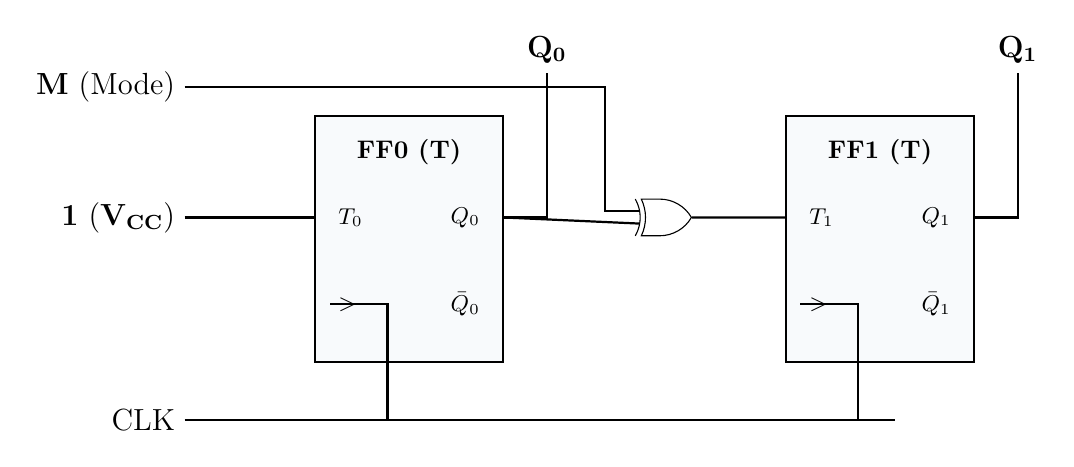
\begin{tikzpicture}[scale=0.92, transform shape]
  % FF0 and FF1
  \draw[thick, fill=boxbg] (1.0, 0) rectangle (3.6, 3.4);
  \node at (2.3, 2.9) {\textbf{FF0 (T)}};
  \node[anchor=west] at (1.2, 2.0) {\small $T_0$};
  \node[anchor=west] at (1.2, 0.8) {\small $>$};
  \node[anchor=east] at (3.4, 2.0) {\small $Q_0$};
  \node[anchor=east] at (3.4, 0.8) {\small $\bar{Q}_0$};

  \draw[thick, fill=boxbg] (7.5, 0) rectangle (10.1, 3.4);
  \node at (8.8, 2.9) {\textbf{FF1 (T)}};
  \node[anchor=west] at (7.7, 2.0) {\small $T_1$};
  \node[anchor=west] at (7.7, 0.8) {\small $>$};
  \node[anchor=east] at (9.9, 2.0) {\small $Q_1$};
  \node[anchor=east] at (9.9, 0.8) {\small $\bar{Q}_1$};

  % Output lines
  \draw[thick] (3.6, 2.0) -- ++(0.6, 0) -- ++(0, 2.0) node[above] {\large $\mathbf{Q_0}$};
  \draw[thick] (10.1, 2.0) -- ++(0.6, 0) -- ++(0, 2.0) node[above] {\large $\mathbf{Q_1}$};

  % T0 = 1
  \draw[thick] (-0.8, 2.0) node[left] {\large $\mathbf{1\ (V_{CC})}$} -- (1.0, 2.0);

  % T1 XOR Gate (M XOR Q0)
  \node[xor gate US, draw, logic gate inputs=nn] (xor1) at (5.8, 2.0) {};
  \draw[thick] (3.6, 2.0) -- (xor1.input 2);
  \draw[thick] (-0.8, 3.8) node[left] {\large $\mathbf{M\ (\text{Mode})}$} -- (5.0, 3.8) |- (xor1.input 1);
  \draw[thick] (xor1.output) -- (7.5, 2.0);

  % Common Synchronous Clock
  \draw[thick] (-0.8, -0.8) node[left] {\large $\mathbf{\text{CLK}}$} -- (9.0, -0.8);
  \draw[thick] (2.0, -0.8) -- (2.0, 0.8) -- (1.2, 0.8);
  \draw[thick] (8.5, -0.8) -- (8.5, 0.8) -- (7.7, 0.8);
\end{tikzpicture}
\end{schematicbox}

\begin{answerbox}
$$\mathbf{T_0 = 1, \qquad T_1 = \bar{M}Q_0 + M\bar{Q}_0 = M \oplus Q_0}$$
\end{answerbox}

\vspace{0.6cm}

% =========================================================================
% QUESTION 6
% =========================================================================
\subsection{Question 6: 4-Bit PISO Shift Register Schematic [3 + 2 = 5 Marks]}
\begin{questionbox}{Problem Statement (2082 Baishakh, Q6)}
Explain the operation of 4-bit parallel-in serial-out (PISO) shift register with necessary circuit and timing diagram for $1101_2$ input data.
\end{questionbox}

A \textbf{Parallel-In Serial-Out (PISO)} shift register loads 4 bits of parallel data simultaneously on a single clock pulse when the mode control line $\text{Shift}/\overline{\text{Load}} = 0$, and shifts data out serially bit-by-bit when $\text{Shift}/\overline{\text{Load}} = 1$.

\paragraph{Steering Logic Equation for Flip-Flop Data Inputs:}
\[
D_i = (\text{Shift} \cdot Q_{i+1}) + (\overline{\text{Load}} \cdot \text{Parallel In}_i)
\]

\begin{schematicbox}{4-Bit Parallel-In Serial-Out (PISO) Shift Register}
\centering
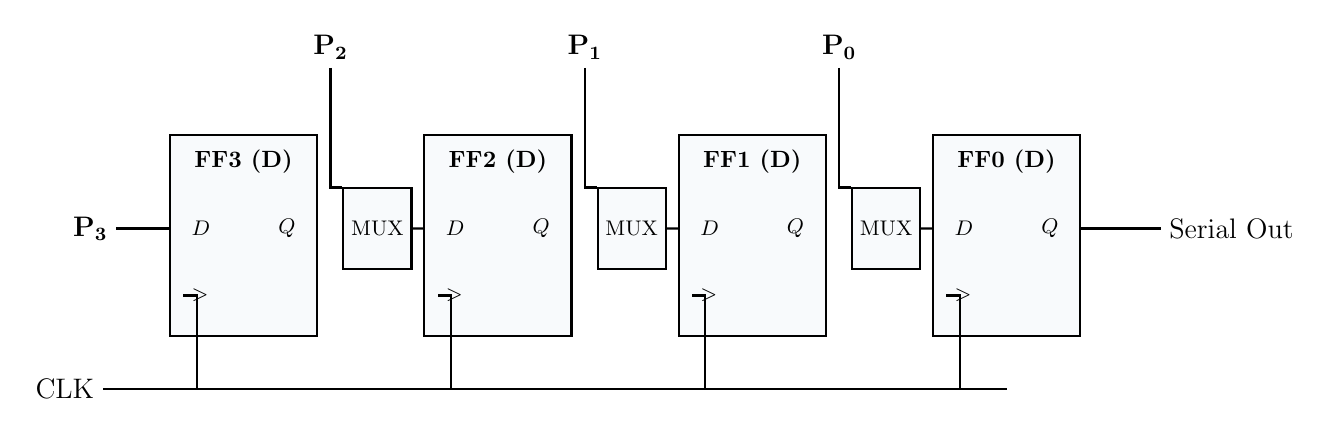
\begin{tikzpicture}[scale=0.85, transform shape]
  % 4 D Flip Flops
  \foreach \i in {3,2,1,0} {
    \draw[thick, fill=boxbg] ({3.8*(3 - \i)}, 0) rectangle ({3.8*(3 - \i) + 2.2}, 3.0);
    \node at ({3.8*(3 - \i) + 1.1}, 2.6) {\textbf{FF\i\ (D)}};
    \node[anchor=west] at ({3.8*(3 - \i) + 0.2}, 1.6) {\small $D$};
    \node[anchor=west] at ({3.8*(3 - \i) + 0.2}, 0.6) {\small $>$};
    \node[anchor=east] at ({3.8*(3 - \i) + 2.0}, 1.6) {\small $Q$};
  }

  % Serial Output from FF0
  \draw[thick] (13.6, 1.6) -- ++(1.2, 0) node[right] {\large $\mathbf{\text{Serial Out}}$};

  % Steering Multiplexers / AND-OR gates
  \foreach \i in {2,1,0} {
    \node[draw, thick, fill=boxbg, minimum width=0.8cm, minimum height=1.2cm] (mux\i) at ({3.8*(3 - \i) - 0.7}, 1.6) {\small MUX};
    \draw[thick] (mux\i.east) -- ({3.8*(3 - \i)}, 1.6);
  }

  % Parallel inputs D3, D2, D1, D0
  \draw[thick] (-0.8, 1.6) node[left] {\large $\mathbf{P_3}$} -- (0, 1.6);
  \draw[thick] (2.4, 4.0) node[above] {\large $\mathbf{P_2}$} |- (mux2.north west);
  \draw[thick] (6.2, 4.0) node[above] {\large $\mathbf{P_1}$} |- (mux1.north west);
  \draw[thick] (10.0, 4.0) node[above] {\large $\mathbf{P_0}$} |- (mux0.north west);

  % Common Clock and Mode Lines
  \draw[thick] (-1.0, -0.8) node[left] {\large $\mathbf{\text{CLK}}$} -- (12.5, -0.8);
  \foreach \i in {0,1,2,3} {
    \draw[thick] ({3.8*\i + 0.4}, -0.8) -- ({3.8*\i + 0.4}, 0.6) -- ({3.8*\i + 0.2}, 0.6);
  }
\end{tikzpicture}
\end{schematicbox}

\paragraph{Cycle-by-Cycle Shifting of Data $1101_2$ ($P_3=1, P_2=1, P_1=0, P_0=1$):}
\begin{center}
\begin{tabular}{|c|c|cccc|c|}
\hline
\textbf{Clock Cycle} & $\mathbf{\text{Shift}/\overline{\text{Load}}}$ & $\mathbf{Q_3}$ & $\mathbf{Q_2}$ & $\mathbf{Q_1}$ & $\mathbf{Q_0}$ & \textbf{Serial Output} \\ \hline
\textbf{Parallel Load} & 0 & 1 & 1 & 0 & 1 & $\mathbf{1}$ (Bit 0 available immediately) \\ \hline
\textbf{Shift 1} & 1 & 0 & 1 & 1 & 0 & $\mathbf{0}$ (Bit 1) \\ \hline
\textbf{Shift 2} & 1 & 0 & 0 & 1 & 1 & $\mathbf{1}$ (Bit 2) \\ \hline
\textbf{Shift 3} & 1 & 0 & 0 & 0 & 1 & $\mathbf{1}$ (Bit 3) \\ \hline
\end{tabular}
\end{center}

\begin{answerbox}
The data word $1101_2$ is loaded in parallel on $\text{Shift}/\overline{\text{Load}}=0$ and shifted out serially as bits $1 \to 0 \to 1 \to 1$ across 3 consecutive shift clock cycles.
\end{answerbox}

\vspace{0.6cm}

% =========================================================================
% QUESTION 7
% =========================================================================
\subsection{Question 7: Mod-12 Asynchronous Counter Schematic [3 + 3 = 6 Marks]}
\begin{questionbox}{Problem Statement (2082 Baishakh, Q7)}
Sketch the circuit diagram of mod-12 asynchronous counter having positive-edge triggering clock system implementing JK flip-flops with neat timing diagram.
\end{questionbox}

A \textbf{Mod-12 Asynchronous Counter} counts 12 states from $0000_2$ ($0_{10}$) to $1011_2$ ($11_{10}$). On the 12th count ($1100_2$, where $Q_3=1, Q_2=1$), an asynchronous active-low clear pulse resets all flip-flops to $0000_2$:
\[
\overline{\text{CLR}} = \overline{Q_3 \cdot Q_2}
\]
With positive-edge triggered flip-flops, UP counting requires ripple clocking via complementary outputs: $\text{CLK}_{i+1} = \bar{Q}_i$.

\begin{schematicbox}{Mod-12 Positive-Edge Triggered Asynchronous Counter}
\centering
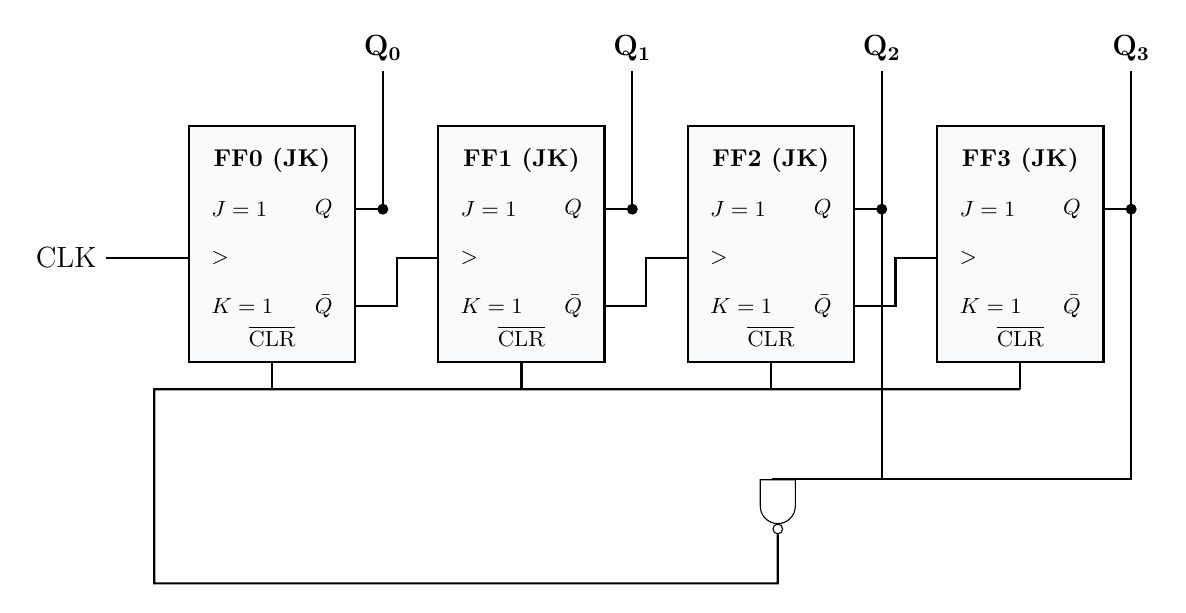
\begin{tikzpicture}[scale=0.88, transform shape]
  % 4 JK Flip Flops
  \foreach \i in {0,1,2,3} {
    \draw[thick, fill=boxbg] ({3.6*\i}, 0) rectangle ({3.6*\i + 2.4}, 3.4);
    \node at ({3.6*\i + 1.2}, 2.9) {\textbf{FF\i\ (JK)}};
    \node[anchor=west] at ({3.6*\i + 0.2}, 2.2) {\small $J=1$};
    \node[anchor=west] at ({3.6*\i + 0.2}, 1.5) {\small $>$};
    \node[anchor=west] at ({3.6*\i + 0.2}, 0.8) {\small $K=1$};
    \node[anchor=east] at ({3.6*\i + 2.2}, 2.2) {\small $Q$};
    \node[anchor=east] at ({3.6*\i + 2.2}, 0.8) {\small $\bar{Q}$};
    \node[anchor=south] at ({3.6*\i + 1.2}, 0.1) {\small $\overline{\text{CLR}}$};

    % Output lines
    \filldraw[black] ({3.6*\i + 2.8}, 2.2) circle (2pt);
    \draw[thick] ({3.6*\i + 2.4}, 2.2) -- ({3.6*\i + 2.8}, 2.2) -- ({3.6*\i + 2.8}, 4.2) node[above] {\large $\mathbf{Q_\i}$};
  }

  % External Clock
  \draw[thick] (-1.2, 1.5) node[left] {\large $\mathbf{\text{CLK}}$} -- (0, 1.5);

  % Ripple connections (Q_bar_i -> CLK_{i+1})
  \draw[thick] (2.4, 0.8) -- (3.0, 0.8) |- (3.6, 1.5);
  \draw[thick] (6.0, 0.8) -- (6.6, 0.8) |- (7.2, 1.5);
  \draw[thick] (9.6, 0.8) -- (10.2, 0.8) |- (10.8, 1.5);

  % Reset NAND Gate: Q3 and Q2
  \node[nand gate US, draw, logic gate inputs=nn, rotate=-90] (nandRst) at (8.5, -2.0) {};
  \draw[thick] (13.6, 2.2) -- (13.6, -1.2) |- (nandRst.input 1); % Q3
  \draw[thick] (10.0, 2.2) -- (10.0, -1.2) |- (nandRst.input 2); % Q2

  % Clear Rail
  \draw[thick] (nandRst.output) -- (8.5, -3.2) -- (-0.5, -3.2) -- (-0.5, -0.4) -- (12.0, -0.4);
  \foreach \i in {0,1,2,3} {
    \draw[thick] ({3.6*\i + 1.2}, -0.4) -- ({3.6*\i + 1.2}, 0);
  }
\end{tikzpicture}
\end{schematicbox}

\begin{answerbox}
Reset condition: $\mathbf{\overline{\text{CLR}} = \overline{Q_3 \cdot Q_2}}$, providing exactly 12 stable counting states from $0000_2$ to $1011_2$.
\end{answerbox}

\vspace{0.6cm}

% =========================================================================
% QUESTION 8
% =========================================================================
\subsection{Question 8: FSM Sequence Detector '010' Using D Flip-Flops [10 Marks]}
\begin{questionbox}{Problem Statement (2082 Baishakh, Q8)}
Design a sequential machine that consists of one input $X$ and one output $Z$. The machine is required to give output high ($Z=1$) whenever it detects the serial sequence of `010' from its input data stream $X$. Implement only D flip-flops for the designed circuit realization.
\end{questionbox}

\paragraph{1. State Definitions (Mealy Model with Overlapping Detection):}
\begin{itemize}
  \item $S_0 (00)$: Reset state / No matching prefix.
  \item $S_1 (01)$: Detected pattern `0'.
  \item $S_2 (10)$: Detected pattern `01'.
  \item When in $S_2$ and next bit is $X=0 \implies$ `010' detected $\implies Z=1$, next state $S_1$ (since trailing `0' can start the next sequence).
\end{itemize}

\begin{schematicbox}{State Diagram for '010' Sequence Detector}
\centering
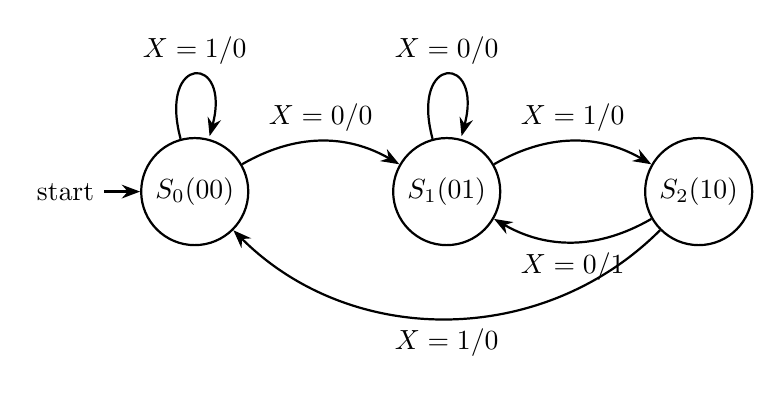
\begin{tikzpicture}[->, >=Stealth, auto, node distance=3.2cm, thick]
  \node[state, initial] (S0) {$S_0 (00)$};
  \node[state] (S1) [right of=S0] {$S_1 (01)$};
  \node[state] (S2) [right of=S1] {$S_2 (10)$};

  \path (S0) edge [loop above] node {$X=1 / 0$} (S0)
             edge [bend left] node {$X=0 / 0$} (S1)
        (S1) edge [loop above] node {$X=0 / 0$} (S1)
             edge [bend left] node {$X=1 / 0$} (S2)
        (S2) edge [bend left=45] node {$X=1 / 0$} (S0)
             edge [bend left] node {$X=0 / 1$} (S1);
\end{tikzpicture}
\end{schematicbox}

\paragraph{2. State Transition and D Excitation Table ($D_1 = Q_1^+, D_0 = Q_0^+$):}
\begin{center}
\begin{tabular}{|cc|c|cc|c|cc|}
\hline
\multicolumn{2}{|c|}{\textbf{Present State}} & \textbf{Input} & \multicolumn{2}{c|}{\textbf{Next State}} & \textbf{Output} & \multicolumn{2}{c|}{\textbf{D Inputs}} \\
$Q_1$ & $Q_0$ & $X$ & $Q_1^+$ & $Q_0^+$ & $\mathbf{Z}$ & $\mathbf{D_1}$ & $\mathbf{D_0}$ \\ \hline
0 & 0 & 0 & 0 & 1 & 0 & 0 & 1 \\ \hline
0 & 0 & 1 & 0 & 0 & 0 & 0 & 0 \\ \hline
0 & 1 & 0 & 0 & 1 & 0 & 0 & 1 \\ \hline
0 & 1 & 1 & 1 & 0 & 0 & 1 & 0 \\ \hline
1 & 0 & 0 & 0 & 1 & 1 & 0 & 1 \\ \hline
1 & 0 & 1 & 0 & 0 & 0 & 0 & 0 \\ \hline
1 & 1 & 0 & $X$ & $X$ & $X$ & $X$ & $X$ \\ \hline
1 & 1 & 1 & $X$ & $X$ & $X$ & $X$ & $X$ \\ \hline
\end{tabular}
\end{center}

\paragraph{3. Minimized Equations via K-Maps:}
\begin{align*}
D_1 &= \bar{Q}_1 Q_0 X \\
D_0 &= \bar{X} \\
Z &= Q_1 \bar{X}
\end{align*}

\begin{schematicbox}{Complete Logic Circuit Realization Using D Flip-Flops}
\centering
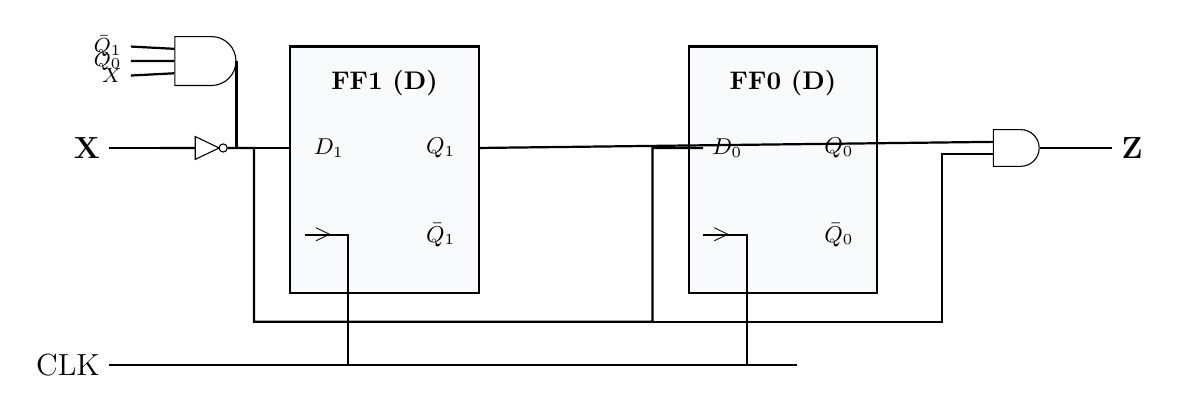
\begin{tikzpicture}[scale=0.92, transform shape]
  % 2 D Flip Flops
  \draw[thick, fill=boxbg] (1.0, 0) rectangle (3.6, 3.4);
  \node at (2.3, 2.9) {\textbf{FF1 (D)}};
  \node[anchor=west] at (1.2, 2.0) {\small $D_1$};
  \node[anchor=west] at (1.2, 0.8) {\small $>$};
  \node[anchor=east] at (3.4, 2.0) {\small $Q_1$};
  \node[anchor=east] at (3.4, 0.8) {\small $\bar{Q}_1$};

  \draw[thick, fill=boxbg] (6.5, 0) rectangle (9.1, 3.4);
  \node at (7.8, 2.9) {\textbf{FF0 (D)}};
  \node[anchor=west] at (6.7, 2.0) {\small $D_0$};
  \node[anchor=west] at (6.7, 0.8) {\small $>$};
  \node[anchor=east] at (8.9, 2.0) {\small $Q_0$};
  \node[anchor=east] at (8.9, 0.8) {\small $\bar{Q}_0$};

  % Input X and Inverter
  \draw[thick] (-1.5, 2.0) node[left] {\large $\mathbf{X}$} -- (-0.8, 2.0);
  \node[not gate US, draw, scale=0.8] (notX) at (-0.2, 2.0) {};
  \draw[thick] (-0.8, 2.0) -- (notX.input);

  % D0 = X_bar
  \draw[thick] (notX.output) -- (0.5, 2.0) -- (0.5, -0.4) -- (6.0, -0.4) |- (6.7, 2.0);

  % D1 = Q1_bar . Q0 . X
  \node[and gate US, draw, logic gate inputs=nnn] (andD1) at (-0.2, 3.2) {};
  \draw[thick] (-1.2, 3.4) node[left] {\footnotesize $\bar{Q}_1$} -- (andD1.input 1);
  \draw[thick] (-1.2, 3.2) node[left] {\footnotesize $Q_0$} -- (andD1.input 2);
  \draw[thick] (-1.2, 3.0) node[left] {\footnotesize $X$} -- (andD1.input 3);
  \draw[thick] (andD1.output) |- (1.0, 2.0);

  % Output Z = Q1 . X_bar
  \node[and gate US, draw, logic gate inputs=nn] (andZ) at (11.0, 2.0) {};
  \draw[thick] (3.6, 2.0) -- (andZ.input 1);
  \draw[thick] (0.5, -0.4) -- (10.0, -0.4) |- (andZ.input 2);
  \draw[thick] (andZ.output) -- ++(1.0, 0) node[right] {\large $\mathbf{Z}$};

  % Clock
  \draw[thick] (-1.5, -1.0) node[left] {\large $\mathbf{\text{CLK}}$} -- (8.0, -1.0);
  \draw[thick] (1.8, -1.0) -- (1.8, 0.8) -- (1.2, 0.8);
  \draw[thick] (7.3, -1.0) -- (7.3, 0.8) -- (6.7, 0.8);
\end{tikzpicture}
\end{schematicbox}

\begin{answerbox}
$$\mathbf{D_1 = \bar{Q}_1 Q_0 X, \qquad D_0 = \bar{X}, \qquad Z = Q_1 \bar{X}}$$
\end{answerbox}

\vspace{0.6cm}

% =========================================================================
% QUESTION 9
% =========================================================================
\subsection{Question 9: Two-Input CMOS NAND Gate Transistor Circuit [4 + 2 = 6 Marks]}
\begin{questionbox}{Problem Statement (2082 Baishakh, Q9)}
Draw the circuit diagram of two-input CMOS NAND gate and explain its logic operation briefly and list the characteristics of TTL logic family.
\end{questionbox}

\paragraph{Part (a): 2-Input CMOS NAND Gate Circuit and Operation [4 Marks]}
A CMOS logic gate consists of a \textbf{Pull-Up Network (PUN)} made of PMOS transistors and a \textbf{Pull-Down Network (PDN)} made of NMOS transistors:
\begin{itemize}
  \item \textbf{PUN:} Two PMOS transistors ($M_1, M_2$) connected in \textbf{parallel} between $V_{DD}$ and Output $Y$.
  \item \textbf{PDN:} Two NMOS transistors ($M_3, M_4$) connected in \textbf{series} between Output $Y$ and Ground.
\end{itemize}

\begin{schematicbox}{Transistor-Level Schematic of 2-Input CMOS NAND Gate}
\centering
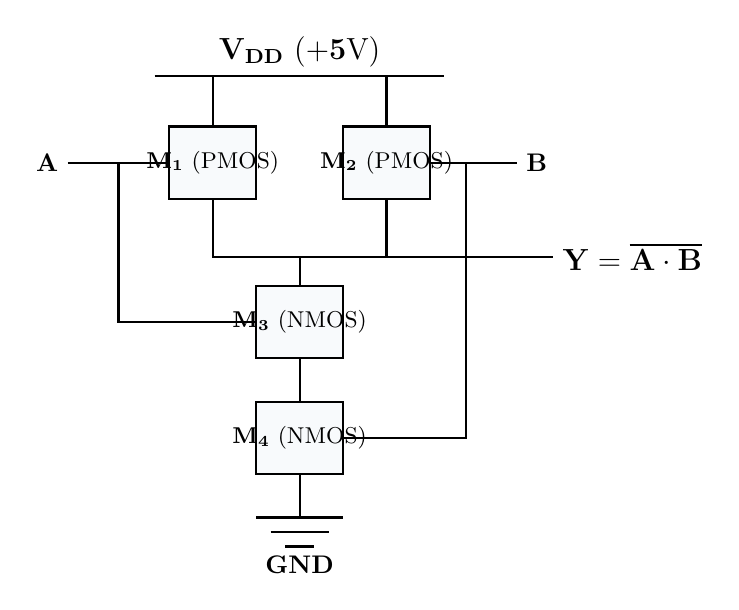
\begin{tikzpicture}[scale=0.92, transform shape]
  % VDD rail
  \draw[thick] (2.0, 5.5) -- (6.0, 5.5);
  \node[above] at (4.0, 5.5) {\large $\mathbf{V_{DD}\ (+5\text{V})}$};

  % PMOS M1 (left) and M2 (right)
  \draw[thick, fill=boxbg] (2.2, 3.8) rectangle (3.4, 4.8);
  \node at (2.8, 4.3) {\small $\mathbf{M_1}$ (PMOS)};
  \draw[thick, fill=boxbg] (4.6, 3.8) rectangle (5.8, 4.8);
  \node at (5.2, 4.3) {\small $\mathbf{M_2}$ (PMOS)};

  \draw[thick] (2.8, 5.5) -- (2.8, 4.8);
  \draw[thick] (5.2, 5.5) -- (5.2, 4.8);

  % Common output Y
  \draw[thick] (2.8, 3.8) -- (2.8, 3.0) -- (5.2, 3.0) -- (5.2, 3.8);
  \draw[thick] (4.0, 3.0) -- (7.5, 3.0) node[right] {\large $\mathbf{Y = \overline{A \cdot B}}$};

  % NMOS M3 (top) and M4 (bottom) in series
  \draw[thick, fill=boxbg] (3.4, 1.6) rectangle (4.6, 2.6);
  \node at (4.0, 2.1) {\small $\mathbf{M_3}$ (NMOS)};
  \draw[thick, fill=boxbg] (3.4, 0.0) rectangle (4.6, 1.0);
  \node at (4.0, 0.5) {\small $\mathbf{M_4}$ (NMOS)};

  \draw[thick] (4.0, 3.0) -- (4.0, 2.6);
  \draw[thick] (4.0, 1.6) -- (4.0, 1.0);
  \draw[thick] (4.0, 0.0) -- (4.0, -0.6);

  % Ground
  \draw[thick] (3.4, -0.6) -- (4.6, -0.6);
  \draw[thick] (3.6, -0.8) -- (4.4, -0.8);
  \draw[thick] (3.8, -1.0) -- (4.2, -1.0);
  \node[below] at (4.0, -1.0) {\textbf{GND}};

  % Inputs A and B
  \draw[thick] (0.8, 4.3) node[left] {$\mathbf{A}$} -- (2.2, 4.3);
  \draw[thick] (0.8, 4.3) -- (1.5, 4.3) |- (3.4, 2.1); % A to M3

  \draw[thick] (7.0, 4.3) node[right] {$\mathbf{B}$} -- (5.8, 4.3);
  \draw[thick] (7.0, 4.3) -- (6.3, 4.3) |- (4.6, 0.5); % B to M4
\end{tikzpicture}
\end{schematicbox}

\paragraph{Operation Truth Table:}
\begin{center}
\begin{tabular}{|cc||cc|cc||c|l|}
\hline
$\mathbf{A}$ & $\mathbf{B}$ & $\mathbf{M_1\ (P)}$ & $\mathbf{M_2\ (P)}$ & $\mathbf{M_3\ (N)}$ & $\mathbf{M_4\ (N)}$ & $\mathbf{Y}$ & \textbf{State} \\ \hline
0 & 0 & ON & ON & OFF & OFF & $\mathbf{1}\ (V_{DD})$ & PUN conducts to $V_{DD}$ \\ \hline
0 & 1 & ON & OFF & OFF & ON & $\mathbf{1}\ (V_{DD})$ & $M_1$ pulls output HIGH \\ \hline
1 & 0 & OFF & ON & ON & OFF & $\mathbf{1}\ (V_{DD})$ & $M_2$ pulls output HIGH \\ \hline
1 & 1 & OFF & OFF & ON & ON & $\mathbf{0}\ (\text{GND})$ & PDN pulls output to Ground \\ \hline
\end{tabular}
\end{center}

\paragraph{Part (b): Characteristics of TTL Logic Family [2 Marks]}
\begin{enumerate}
  \item \textbf{Supply Voltage:} Standard $V_{CC} = +5.0\text{V} \pm 5\%$.
  \item \textbf{Power Dissipation:} $\approx 10\text{ mW}$ per gate (Standard 7400 TTL).
  \item \textbf{Propagation Delay:} $\approx 10\text{ ns}$ (high speed bipolar technology).
  \item \textbf{Noise Margin:} $NM_H = 0.4\text{V}, NM_L = 0.4\text{V}$.
  \item \textbf{Fan-Out:} 10 standard 7400 TTL loads.
\end{enumerate}

\begin{answerbox}
CMOS NAND uses parallel PMOS pull-up and series NMOS pull-down transistors, providing near-zero static power dissipation and full rail-to-rail voltage swing.
\end{answerbox}

\vspace{0.6cm}

% =========================================================================
% QUESTION 10
% =========================================================================
\subsection{Question 10: Time Interval Measurement Block Diagram [4 Marks]}
\begin{questionbox}{Problem Statement (2082 Baishakh, Q10)}
With the help of functional diagram explain the operation of time measuring circuit.
\end{questionbox}

A \textbf{Digital Time Interval Meter} measures the elapsed time $\Delta T$ between a START trigger event and a STOP trigger event by counting the number of precision clock pulses of known period $T_0$:
\[
\Delta T = N \times T_0 = \frac{N}{f_{\text{osc}}}
\]

\paragraph{Operational Sequence:}
\begin{enumerate}
  \item \textbf{Start Pulse Conditioning:} The START signal passes through an input amplifier and Schmitt trigger, setting the \textbf{Gate Control Flip-Flop (RS Latch)}.
  \item \textbf{Gating Period:} While the latch is SET ($Q=1$), the \textbf{Main AND Gate} opens, allowing clock pulses from the crystal oscillator time base to flow into the decade counters.
  \item \textbf{Stop Pulse Conditioning:} The arrival of the STOP event resets the latch ($Q=0$), closing the AND gate and freezing the count.
  \item \textbf{Display:} The accumulated count $N$ is displayed directly on 7-segment digital readouts in microseconds ($\mu$s), milliseconds (ms), or seconds (s).
\end{enumerate}

\begin{schematicbox}{Functional Block Diagram of Digital Time Interval Measurement Circuit}
\centering
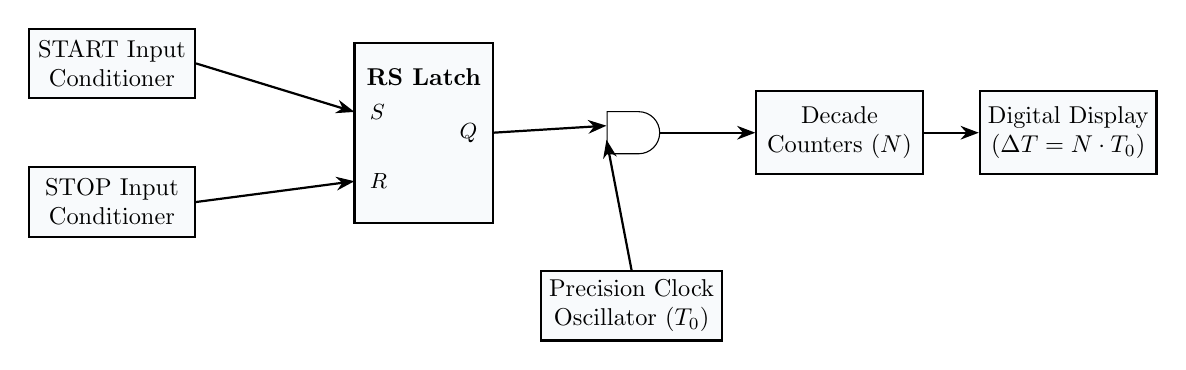
\begin{tikzpicture}[scale=0.88, transform shape, >=Stealth]
  % Start / Stop input blocks
  \node[draw, thick, fill=boxbg, minimum width=2.4cm, minimum height=1.0cm, align=center] (start) at (0, 3.5) {START Input\\Conditioner};
  \node[draw, thick, fill=boxbg, minimum width=2.4cm, minimum height=1.0cm, align=center] (stop) at (0, 1.5) {STOP Input\\Conditioner};

  % RS Flip Flop
  \draw[thick, fill=boxbg] (3.5, 1.2) rectangle (5.5, 3.8);
  \node at (4.5, 3.3) {\textbf{RS Latch}};
  \node[anchor=west] at (3.6, 2.8) {\small $S$};
  \node[anchor=west] at (3.6, 1.8) {\small $R$};
  \node[anchor=east] at (5.4, 2.5) {\small $Q$};

  \draw[thick, ->] (start.east) -- (3.5, 2.8);
  \draw[thick, ->] (stop.east) -- (3.5, 1.8);

  % Main AND Gate
  \node[and gate US, draw, logic gate inputs=nn, scale=1.2] (mainGate) at (7.5, 2.5) {};
  \draw[thick, ->] (5.5, 2.5) -- (mainGate.input 1);

  % Time base oscillator
  \node[draw, thick, fill=boxbg, minimum width=2.2cm, minimum height=1.0cm, align=center] (osc) at (7.5, 0.0) {Precision Clock\\Oscillator ($T_0$)};
  \draw[thick, ->] (osc.north) -- (mainGate.input 2);

  % Counter and Display
  \node[draw, thick, fill=boxbg, minimum width=2.4cm, minimum height=1.2cm, align=center] (counter) at (10.5, 2.5) {Decade\\Counters ($N$)};
  \node[draw, thick, fill=boxbg, minimum width=2.2cm, minimum height=1.2cm, align=center] (disp) at (13.8, 2.5) {Digital Display\\($\Delta T = N \cdot T_0$)};

  \draw[thick, ->] (mainGate.output) -- (counter.west);
  \draw[thick, ->] (counter.east) -- (disp.west);
\end{tikzpicture}
\end{schematicbox}

\begin{answerbox}
The time interval measurement system gates standard clock pulses between START and STOP triggers, computing time elapsed as $\mathbf{\Delta T = N \times T_0}$.
\end{answerbox}

\chapter{2081 Ashwin Examination Solutions}

\section*{Examination Overview}
\begin{tabular}{@{}ll@{}}
\textbf{Level:} Bachelor in Engineering (BE) & \textbf{Full Marks:} 60 \\
\textbf{Programme:} BEI, BCT & \textbf{Pass Marks:} 24 \\
\textbf{Year / Part:} I / II & \textbf{Time:} 3 Hours \\
\textbf{Subject:} Digital Logic (ENEX 152) & \textbf{Examination Type:} Regular (New Course - 2080 Batch) \\
\end{tabular}

\vspace{0.6cm}
\hrule
\vspace{0.6cm}

% =========================================================================
% QUESTION 1
% =========================================================================
\subsection{Question 1: Merits \& Demerits of Digital Signals [2 Marks]}
\begin{questionbox}{Problem Statement (2081 Ashwin, Q1)}
Mention merits and demerits of digital signal over analog signal.
\end{questionbox}

\paragraph{Merits of Digital Signals:}
\begin{enumerate}
  \item \textbf{Superior Noise Immunity:} Digital circuits distinguish only discrete voltage bands (`0' and `1'). As long as noise voltage does not exceed the logic threshold, signal integrity is perfectly regenerated by repeaters.
  \item \textbf{Lossless Storage and Reproduction:} Data stored in semiconductor memory or optical media can be retrieved and duplicated indefinitely without analog degradation.
  \item \textbf{Advanced Error Detection and Correction:} Robust mathematical codes (Parity, CRC, Hamming, Reed-Solomon) can detect and correct bit errors caused during transmission.
  \item \textbf{Programmability and Integration:} Standard digital VLSI architectures (FPGA, DSP, Microprocessors) allow flexible software reconfigurability and massive circuit density.
\end{enumerate}

\paragraph{Demerits of Digital Signals:}
\begin{enumerate}
  \item \textbf{Higher Bandwidth Requirement:} Transmitting digital square pulses requires significantly wider channel bandwidth than transmitting the raw baseband analog waveform.
  \item \textbf{Quantization Error:} Analog-to-Digital Conversion (ADC) introduces unavoidable quantization noise due to finite bit resolution.
  \item \textbf{System Complexity:} Requires ADC and DAC conversion stages at real-world physical interfaces.
\end{enumerate}

\begin{answerbox}
Digital signals provide unmatched noise immunity, lossless storage, and error correction at the expense of higher transmission bandwidth and quantization artifacts.
\end{answerbox}

\vspace{0.6cm}

% =========================================================================
% QUESTION 2
% =========================================================================
\subsection{Question 2: Radix \& Gray Code Conversions [1.5 + 1.5 = 3 Marks]}
\begin{questionbox}{Problem Statement (2081 Ashwin, Q2)}
Perform the following as indicated:
\begin{enumerate}[label=(\alph*)]
  \item $(6E.2C)_{16} = (?)_{8}$
  \item $(10110110)_{\text{Gray}} = (?)_{2}$
\end{enumerate}
\end{questionbox}

\paragraph{Part (a): Hexadecimal to Octal Conversion: $(6E.2C)_{16} \to (?)_{8}$ [1.5 Marks]}
\begin{enumerate}
  \item \textbf{Convert Hexadecimal to 4-bit Binary:}
  \[
  6_{16} = 0110_2, \quad E_{16} = 1110_2, \quad 2_{16} = 0010_2, \quad C_{16} = 1100_2
  \]
  \[
  (6E.2C)_{16} = (0110\ 1110\ .\ 0010\ 1100)_2
  \]
  \item \textbf{Regroup into 3-bit Octal Groups:}
  \begin{itemize}
    \item \textbf{Integer part (grouping leftward from radix point):}
    \[
    \underbrace{001}_{1}\ \underbrace{101}_{5}\ \underbrace{110}_{6} \implies (156)_8
    \]
    \item \textbf{Fractional part (grouping rightward from radix point):}
    \[
    \underbrace{001}_{1}\ \underbrace{011}_{3}\ \underbrace{000}_{0} \implies (.130)_8 = (.13)_8
    \]
  \end{itemize}
\end{enumerate}
Thus, $(6E.2C)_{16} = \mathbf{(156.13)_8}$.

\paragraph{Part (b): Gray Code to Binary Conversion: $(10110110)_{\text{Gray}} \to (?)_{2}$ [1.5 Marks]}
Given $g_7 g_6 g_5 g_4 g_3 g_2 g_1 g_0 = 10110110_2$:
\begin{itemize}
  \item $b_7 = g_7 = 1$
  \item $b_6 = b_7 \oplus g_6 = 1 \oplus 0 = 1$
  \item $b_5 = b_6 \oplus g_5 = 1 \oplus 1 = 0$
  \item $b_4 = b_5 \oplus g_4 = 0 \oplus 1 = 1$
  \item $b_3 = b_4 \oplus g_3 = 1 \oplus 0 = 1$
  \item $b_2 = b_3 \oplus g_2 = 1 \oplus 1 = 0$
  \item $b_1 = b_2 \oplus g_1 = 0 \oplus 1 = 1$
  \item $b_0 = b_1 \oplus g_0 = 1 \oplus 0 = 1$
\end{itemize}
Thus, $(10110110)_{\text{Gray}} = \mathbf{(11011011)_2}$.

\begin{answerbox}
\begin{align*}
\text{(a)}\quad (6E.2C)_{16} &= \mathbf{(156.13)_8} \\
\text{(b)}\quad (10110110)_{\text{Gray}} &= \mathbf{(11011011)_2}
\end{align*}
\end{answerbox}

\vspace{0.6cm}

% =========================================================================
% QUESTION 3
% =========================================================================
\subsection{Question 3: BCD to 7-Segment 'f' Segment Decoder Logic Circuit [4 Marks]}
\begin{questionbox}{Problem Statement (2081 Ashwin, Q3)}
Design the simplest logic circuit for `$f$' segment for the BCD-to-seven segment display decoder.
\end{questionbox}

A 7-segment display uses LED segments $a, b, c, d, e, f, g$. The `$f$' segment represents the upper-left vertical LED segment, which must be illuminated (HIGH) for decimal digits \textbf{0, 4, 5, 6, 8, 9}.

\paragraph{1. Truth Table for Segment $f(A, B, C, D)$ (where $A$ is MSB):}
\begin{center}
\small
\begin{tabular}{|c|cccc||c|l|}
\hline
\textbf{Decimal Digit} & $A$ & $B$ & $C$ & $D$ & $\mathbf{f}$ & \textbf{Display Appearance} \\ \hline
0 & 0 & 0 & 0 & 0 & \textbf{1} & Illuminated \\ \hline
1 & 0 & 0 & 0 & 1 & \textbf{0} & Off \\ \hline
2 & 0 & 0 & 1 & 0 & \textbf{0} & Off \\ \hline
3 & 0 & 0 & 1 & 1 & \textbf{0} & Off \\ \hline
4 & 0 & 1 & 0 & 0 & \textbf{1} & Illuminated \\ \hline
5 & 0 & 1 & 0 & 1 & \textbf{1} & Illuminated \\ \hline
6 & 0 & 1 & 1 & 0 & \textbf{1} & Illuminated \\ \hline
7 & 0 & 1 & 1 & 1 & \textbf{0} & Off \\ \hline
8 & 1 & 0 & 0 & 0 & \textbf{1} & Illuminated \\ \hline
9 & 1 & 0 & 0 & 1 & \textbf{1} & Illuminated \\ \hline
10--15 & \multicolumn{4}{c||}{\text{Invalid BCD Codes}} & $\mathbf{X}$ & Don't Cares ($d_{10} \dots d_{15}$) \\ \hline
\end{tabular}
\end{center}

\paragraph{2. 4-Variable K-Map Minimization:}
\begin{center}
\begin{tabular}{|c|c|c|c|c|}
\hline
$AB \ \backslash \ CD$ & \textbf{00} & \textbf{01} & \textbf{11} & \textbf{10} \\ \hline
\textbf{00} & $\mathbf{1}\ (m_0)$ & $0\ (m_1)$ & $0\ (m_3)$ & $0\ (m_2)$ \\ \hline
\textbf{01} & $\mathbf{1}\ (m_4)$ & $\mathbf{1}\ (m_5)$ & $0\ (m_7)$ & $\mathbf{1}\ (m_6)$ \\ \hline
\textbf{11} & $\mathbf{X}\ (d_{12})$ & $\mathbf{X}\ (d_{13})$ & $\mathbf{X}\ (d_{15})$ & $\mathbf{X}\ (d_{14})$ \\ \hline
\textbf{10} & $\mathbf{1}\ (m_8)$ & $\mathbf{1}\ (m_9)$ & $\mathbf{X}\ (d_{11})$ & $\mathbf{X}\ (d_{10})$ \\ \hline
\end{tabular}
\end{center}

\paragraph{Groupings:}
\begin{enumerate}
  \item \textbf{Group 1 (Octet in rows 11 \& 10):} $(m_8, m_9, d_{10}, d_{11}, d_{12}, d_{13}, d_{14}, d_{15}) \implies \mathbf{A}$.
  \item \textbf{Group 2 (Quad in columns 00 \& 01, rows 01 \& 11):} $(m_4, m_5, d_{12}, d_{13}) \implies \mathbf{B\bar{C}}$.
  \item \textbf{Group 3 (Quad in column 00):} $(m_0, m_4, d_{12}, m_8) \implies \mathbf{\bar{C}\bar{D}}$.
  \item \textbf{Group 4 (Quad across rows 01 \& 11, cols 00 \& 10):} $(m_4, m_6, d_{12}, d_{14}) \implies \mathbf{B\bar{D}}$.
\end{enumerate}

\paragraph{Minimal Boolean Expression:}
\[
\mathbf{f = A + B\bar{C} + B\bar{D} + \bar{C}\bar{D}}
\]

\begin{schematicbox}{Logic Circuit Realization for Segment 'f'}
\centering
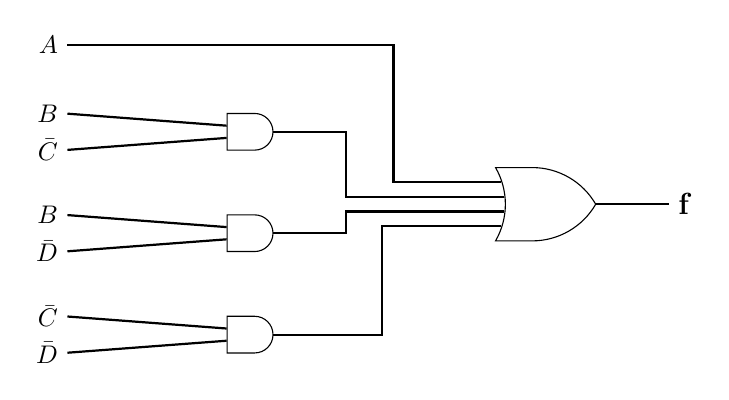
\begin{tikzpicture}[scale=0.92, transform shape]
  % 3 AND Gates
  \node[and gate US, draw, logic gate inputs=nn] (and1) at (3.5, 3.2) {};
  \node[and gate US, draw, logic gate inputs=nn] (and2) at (3.5, 1.8) {};
  \node[and gate US, draw, logic gate inputs=nn] (and3) at (3.5, 0.4) {};

  % Inputs
  \draw[thick] (1.0, 3.45) node[left] {$B$} -- (and1.input 1);
  \draw[thick] (1.0, 2.95) node[left] {$\bar{C}$} -- (and1.input 2);

  \draw[thick] (1.0, 2.05) node[left] {$B$} -- (and2.input 1);
  \draw[thick] (1.0, 1.55) node[left] {$\bar{D}$} -- (and2.input 2);

  \draw[thick] (1.0, 0.65) node[left] {$\bar{C}$} -- (and3.input 1);
  \draw[thick] (1.0, 0.15) node[left] {$\bar{D}$} -- (and3.input 2);

  % 4-input OR gate
  \node[or gate US, draw, logic gate inputs=nnnn, scale=1.2] (orgate) at (7.5, 2.2) {};
  \draw[thick] (1.0, 4.4) node[left] {$A$} -- (5.5, 4.4) |- (orgate.input 1);
  \draw[thick] (and1.output) -- ++(1.0, 0) |- (orgate.input 2);
  \draw[thick] (and2.output) -- ++(1.0, 0) |- (orgate.input 3);
  \draw[thick] (and3.output) -- ++(1.5, 0) |- (orgate.input 4);

  \draw[thick] (orgate.output) -- ++(1.0, 0) node[right] {\large $\mathbf{f}$};
\end{tikzpicture}
\end{schematicbox}

\begin{answerbox}
$$\mathbf{f = A + B\bar{C} + B\bar{D} + \bar{C}\bar{D}}$$
\end{answerbox}

\vspace{0.6cm}

% =========================================================================
% QUESTION 4
% =========================================================================
\subsection{Question 4: 4:1 MUX Realization \& Combined Adder/Subtractor [3 + 7 = 10 Marks]}
\begin{questionbox}{Problem Statement (2081 Ashwin, Q4)}
Implement $Y(A, B, C) = \sum m(0, 2, 3, 5, 7)$ using only a single $4:1$ MUX. Design a circuit which can realize both the half-adder and the half-subtractor in a single circuit.
\end{questionbox}

\paragraph{Part (a): Realize $Y(A, B, C) = \sum m(0, 2, 3, 5, 7)$ Using Single $4:1$ MUX [3 Marks]}
Let select lines be $S_1 = A, S_0 = B$:
\begin{center}
\begin{tabular}{|c|c|c|c|}
\hline
\textbf{Select Inputs} $(A, B)$ & \textbf{Minterms Included} & \textbf{Function Output $Y$} & \textbf{Data Input Line} \\ \hline
$00$ & $m_0(\bar{C}) + m_1(C) \to m_0$ & $\bar{C}$ & $\mathbf{I_0 = \bar{C}}$ \\ \hline
$01$ & $m_2(\bar{C}) + m_3(C) \to m_2, m_3$ & $\bar{C} + C = 1$ & $\mathbf{I_1 = 1\ (V_{CC})}$ \\ \hline
$10$ & $m_4(\bar{C}) + m_5(C) \to m_5$ & $C$ & $\mathbf{I_2 = C}$ \\ \hline
$11$ & $m_6(\bar{C}) + m_7(C) \to m_7$ & $C$ & $\mathbf{I_3 = C}$ \\ \hline
\end{tabular}
\end{center}

\begin{schematicbox}{4:1 Multiplexer Realization for $Y(A,B,C) = \sum m(0,2,3,5,7)$}
\centering
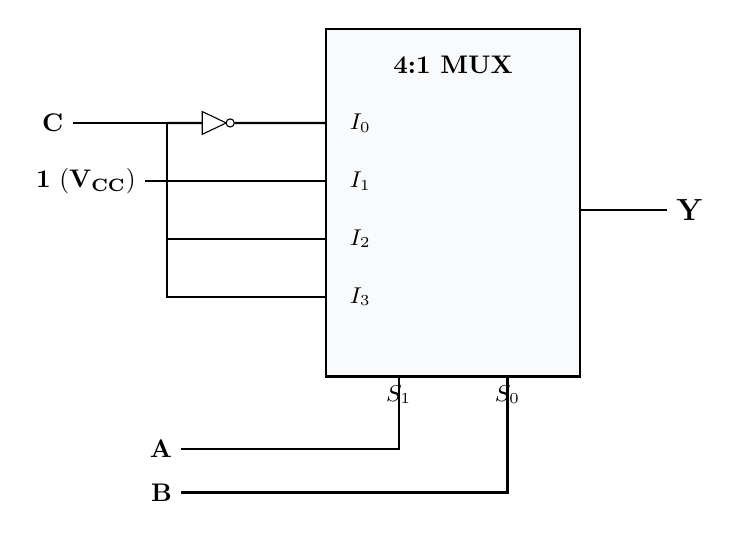
\begin{tikzpicture}[scale=0.92, transform shape]
  % 4:1 MUX Box
  \draw[thick, fill=boxbg] (3.0, 0) rectangle (6.5, 4.8);
  \node at (4.75, 4.3) {\textbf{4:1 MUX}};
  \node[anchor=west] at (3.2, 3.5) {\small $I_0$};
  \node[anchor=west] at (3.2, 2.7) {\small $I_1$};
  \node[anchor=west] at (3.2, 1.9) {\small $I_2$};
  \node[anchor=west] at (3.2, 1.1) {\small $I_3$};
  \node[anchor=north] at (4.0, 0) {\small $S_1$};
  \node[anchor=north] at (5.5, 0) {\small $S_0$};

  \draw[thick] (6.5, 2.3) -- ++(1.2, 0) node[right] {\large $\mathbf{Y}$};

  % NOT Gate for C_bar
  \draw[thick] (-0.5, 3.5) node[left] {$\mathbf{C}$} -- (0.8, 3.5);
  \node[not gate US, draw, scale=0.8] (notC) at (1.4, 3.5) {};
  \draw[thick] (0.8, 3.5) -- (notC.input);
  \draw[thick] (notC.output) -- (3.0, 3.5);

  \draw[thick] (0.5, 2.7) node[left] {$\mathbf{1\ (V_{CC})}$} -- (3.0, 2.7);
  \draw[thick] (0.8, 3.5) -- (0.8, 1.9) -- (3.0, 1.9);
  \draw[thick] (0.8, 1.9) -- (0.8, 1.1) -- (3.0, 1.1);

  % Select Inputs A, B
  \draw[thick] (1.0, -1.0) node[left] {$\mathbf{A}$} -- (4.0, -1.0) -- (4.0, 0);
  \draw[thick] (1.0, -1.6) node[left] {$\mathbf{B}$} -- (5.5, -1.6) -- (5.5, 0);
\end{tikzpicture}
\end{schematicbox}

\paragraph{Part (b): Combined Half-Adder and Half-Subtractor in a Single Circuit [7 Marks]}
Let $A$ and $B$ be the two 1-bit binary inputs, and let $M$ be the mode control line:
\begin{itemize}
  \item \textbf{Mode $M = 0$ (Half-Adder):}
  \[
  \text{Sum } S = A \oplus B, \qquad \text{Carry } C = A \cdot B
  \]
  \item \textbf{Mode $M = 1$ (Half-Subtractor):}
  \[
  \text{Difference } D = A \oplus B, \qquad \text{Borrow } B_{\text{out}} = \bar{A} \cdot B
  \]
\end{itemize}
\textbf{Key Insight:} The first output is identical in both operations: $\mathbf{\text{Sum} / \text{Difference} = A \oplus B}$.\\
The second output ($\text{Carry} / \text{Borrow}$) requires $A \cdot B$ when $M=0$ and $\bar{A} \cdot B$ when $M=1$. Using an XOR gate with mode control $M$:
\[
(A \oplus M) = \begin{cases} A \oplus 0 = A & \text{when } M = 0 \\ A \oplus 1 = \bar{A} & \text{when } M = 1 \end{cases}
\]
Therefore, the combined Carry / Borrow output equation is:
\[
\mathbf{\text{Carry} / \text{Borrow} = (A \oplus M) \cdot B}
\]

\begin{schematicbox}{Combined Half-Adder and Half-Subtractor Circuit Schematic}
\centering
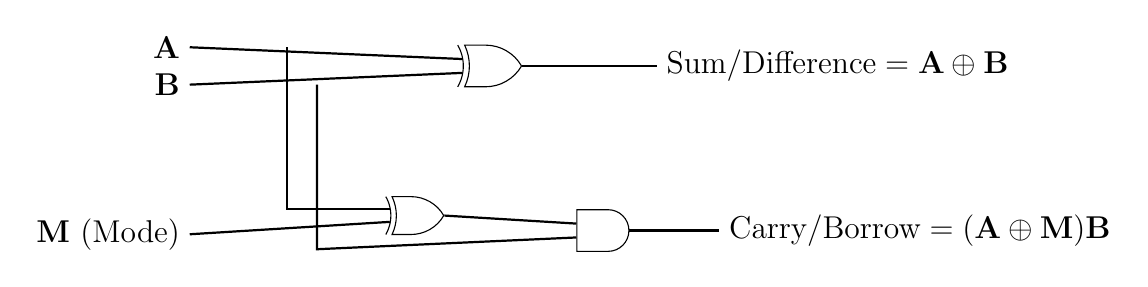
\begin{tikzpicture}[scale=0.95, transform shape]
  % XOR 1 for Sum / Difference
  \node[xor gate US, draw, logic gate inputs=nn, scale=1.1] (xorSum) at (4.5, 3.2) {};
  \draw[thick] (0.5, 3.45) node[left] {\large $\mathbf{A}$} -- (xorSum.input 1);
  \draw[thick] (0.5, 2.95) node[left] {\large $\mathbf{B}$} -- (xorSum.input 2);
  \draw[thick] (xorSum.output) -- ++(1.8, 0) node[right] {\large $\mathbf{\text{Sum} / \text{Difference} = A \oplus B}$};

  % XOR 2 for Mode Control (A XOR M)
  \node[xor gate US, draw, logic gate inputs=nn, scale=1.0] (xorM) at (3.5, 1.2) {};
  \draw[thick] (1.8, 3.45) |- (xorM.input 1);
  \draw[thick] (0.5, 0.95) node[left] {\large $\mathbf{M\ (\text{Mode})}$} -- (xorM.input 2);

  % AND Gate for Carry / Borrow
  \node[and gate US, draw, logic gate inputs=nn, scale=1.1] (andCB) at (6.0, 1.0) {};
  \draw[thick] (xorM.output) -- (andCB.input 1);
  \draw[thick] (2.2, 2.95) -- (2.2, 0.75) -- (andCB.input 2);
  \draw[thick] (andCB.output) -- ++(1.2, 0) node[right] {\large $\mathbf{\text{Carry} / \text{Borrow} = (A \oplus M)B}$};
\end{tikzpicture}
\end{schematicbox}

\begin{answerbox}
\textbf{4:1 MUX Inputs:} $I_0 = \bar{C}, I_1 = 1, I_2 = C, I_3 = C$ with $S_1 = A, S_0 = B$.\\
\textbf{Combined Adder/Subtractor Equations:}
$$\mathbf{\text{Sum} / \text{Difference} = A \oplus B, \qquad \text{Carry} / \text{Borrow} = (A \oplus M) \cdot B}$$
\end{answerbox}

\vspace{0.6cm}

% =========================================================================
% QUESTION 5
% =========================================================================
\subsection{Question 5: Mod-6 Synchronous DOWN Counter Schematic [7 Marks]}
\begin{questionbox}{Problem Statement (2081 Ashwin, Q5)}
Design a mod-6 synchronous down counter using JK flip-flops.
\end{questionbox}

A \textbf{Mod-6 Synchronous DOWN Counter} counts backward through 6 states:
\[
5 \to 4 \to 3 \to 2 \to 1 \to 0 \to 5 \quad (101_2 \to 100_2 \to 011_2 \to 010_2 \to 001_2 \to 000_2 \to 101_2)
\]
Requires $N = 3$ flip-flops ($Q_2, Q_1, Q_0$). Unused states: $110_2$ and $111_2$ (treated as Don't Cares).

\paragraph{1. State Transition and JK Excitation Table:}
\begin{center}
\begin{tabular}{|c|ccc|ccc|cccccc|}
\hline
\textbf{State} & \multicolumn{3}{c|}{\textbf{Present State}} & \multicolumn{3}{c|}{\textbf{Next State}} & \multicolumn{6}{c|}{\textbf{JK Flip-Flop Inputs}} \\
& $Q_2$ & $Q_1$ & $Q_0$ & $Q_2^+$ & $Q_1^+$ & $Q_0^+$ & $\mathbf{J_2}$ & $\mathbf{K_2}$ & $\mathbf{J_1}$ & $\mathbf{K_1}$ & $\mathbf{J_0}$ & $\mathbf{K_0}$ \\ \hline
5 & 1 & 0 & 1 & 1 & 0 & 0 & $X$ & 0 & 0 & $X$ & $X$ & 1 \\ \hline
4 & 1 & 0 & 0 & 0 & 1 & 1 & $X$ & 1 & 1 & $X$ & 1 & $X$ \\ \hline
3 & 0 & 1 & 1 & 0 & 1 & 0 & 0 & $X$ & $X$ & 0 & $X$ & 1 \\ \hline
2 & 0 & 1 & 0 & 0 & 0 & 1 & 0 & $X$ & $X$ & 1 & 1 & $X$ \\ \hline
1 & 0 & 0 & 1 & 0 & 0 & 0 & 0 & $X$ & 0 & $X$ & $X$ & 1 \\ \hline
0 & 0 & 0 & 0 & 1 & 0 & 1 & 1 & $X$ & 0 & $X$ & 1 & $X$ \\ \hline
\end{tabular}
\end{center}

\paragraph{2. Minimized JK Equations via K-Maps:}
\begin{itemize}
  \item $\mathbf{J_0 = 1, \qquad K_0 = 1}$ (LSB toggles every single clock edge).
  \item $\mathbf{J_1 = \bar{Q}_2 \bar{Q}_0, \qquad K_1 = \bar{Q}_0}$.
  \item $\mathbf{J_2 = \bar{Q}_1 \bar{Q}_0, \qquad K_2 = \bar{Q}_1 \bar{Q}_0}$ (or $K_2 = \bar{Q}_0$).
\end{itemize}

\paragraph{3. Lock-out and Self-Starting Verification:}
\begin{itemize}
  \item If counter powers up in state $110_2$: $Q_2^+=1, Q_1^+=0, Q_0^+=1 \implies \text{Next State } 101_2$ (Valid state!).
  \item If counter powers up in state $111_2$: $Q_2^+=1, Q_1^+=1, Q_0^+=0 \implies \text{Next State } 110_2 \to 101_2$ (Valid state!).
\end{itemize}

\begin{schematicbox}{Mod-6 Synchronous DOWN Counter Logic Circuit}
\centering
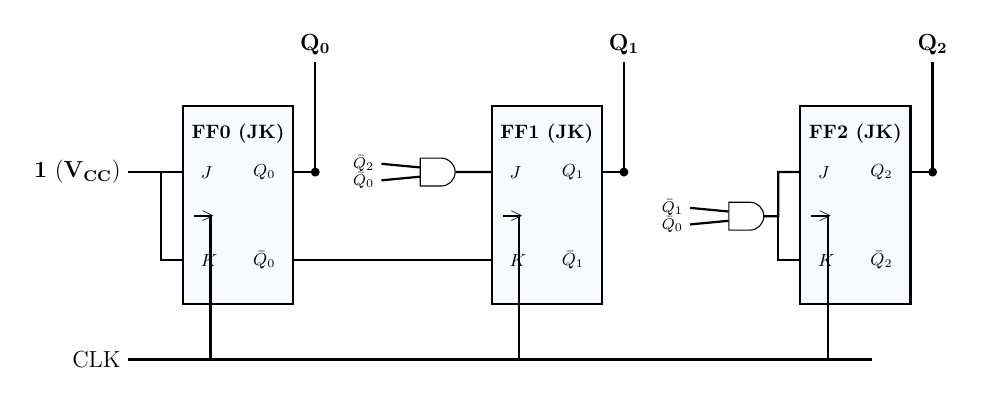
\begin{tikzpicture}[scale=0.70, transform shape]
  % 3 JK Flip Flops (Width 2.0 each, wide 3.6cm inter-stage gaps)
  % FF0: x in [0, 2.0]
  % FF1: x in [5.6, 7.6]
  % FF2: x in [11.2, 13.2]
  \foreach \i/\xpos in {0/0, 1/5.6, 2/11.2} {
    \draw[thick, fill=boxbg] (\xpos, 0) rectangle (\xpos + 2.0, 3.6);
    \node at (\xpos + 1.0, 3.1) {\textbf{FF\i\ (JK)}};
    \node[anchor=west] at (\xpos + 0.2, 2.4) {\small $J$};
    \node[anchor=west] at (\xpos + 0.2, 1.6) {\small $>$};
    \node[anchor=west] at (\xpos + 0.2, 0.8) {\small $K$};
    \node[anchor=east] at (\xpos + 1.8, 2.4) {\small $Q_\i$};
    \node[anchor=east] at (\xpos + 1.8, 0.8) {\small $\bar{Q}_\i$};

    \filldraw[black] (\xpos + 2.4, 2.4) circle (2pt);
    \draw[thick] (\xpos + 2.0, 2.4) -- (\xpos + 2.4, 2.4) -- (\xpos + 2.4, 4.4) node[above] {\large $\mathbf{Q_\i}$};
  }

  % J0 = K0 = 1 (VCC)
  \draw[thick] (-1.0, 2.4) node[left] {\large $\mathbf{1\ (V_{CC})}$} -- (0, 2.4);
  \draw[thick] (-0.4, 2.4) |- (0, 0.8);

  % Common Synchronous Clock Rail
  \draw[thick] (-1.0, -1.0) node[left] {\large $\mathbf{\text{CLK}}$} -- (12.5, -1.0);
  \foreach \xpos in {0, 5.6, 11.2} {
    \draw[thick] (\xpos + 0.5, -1.0) -- (\xpos + 0.5, 1.6) -- (\xpos + 0.2, 1.6);
  }

  % AND Gate for J1 = Q2_bar . Q0_bar (in gap [2.0, 5.6])
  \node[and gate US, draw, logic gate inputs=nn] (andJ1) at (4.6, 2.4) {};
  \draw[thick] (3.6, 2.55) node[left] {\footnotesize $\bar{Q}_2$} -- (andJ1.input 1);
  \draw[thick] (3.6, 2.25) node[left] {\footnotesize $\bar{Q}_0$} -- (andJ1.input 2);
  \draw[thick] (andJ1.output) -- (5.6, 2.4);

  % K1 = Q0_bar
  \draw[thick] (2.0, 0.8) -- (2.6, 0.8) -- (2.6, 0.8) |- (5.6, 0.8);

  % AND Gate for J2 = K2 = Q1_bar . Q0_bar (in gap [7.6, 11.2])
  \node[and gate US, draw, logic gate inputs=nn] (and2) at (10.2, 1.6) {};
  \draw[thick] (9.2, 1.75) node[left] {\footnotesize $\bar{Q}_1$} -- (and2.input 1);
  \draw[thick] (9.2, 1.45) node[left] {\footnotesize $\bar{Q}_0$} -- (and2.input 2);
  \draw[thick] (and2.output) -- (10.8, 1.6) |- (11.2, 2.4);
  \draw[thick] (10.8, 1.6) |- (11.2, 0.8);
\end{tikzpicture}
\end{schematicbox}

\begin{answerbox}
$$\mathbf{J_0 = 1, \ K_0 = 1, \quad J_1 = \bar{Q}_2\bar{Q}_0, \ K_1 = \bar{Q}_0, \quad J_2 = K_2 = \bar{Q}_1\bar{Q}_0}$$
\end{answerbox}

\vspace{0.6cm}

% =========================================================================
% QUESTION 7
% =========================================================================
\subsection{Question 7: 4-Bit SIPO Shift Register Schematic \& Waveforms [5 Marks]}
\begin{questionbox}{Problem Statement (2081 Ashwin, Q7)}
Explain the working of 4-bit SIPO shift register with timing diagram for data input `1011'.
\end{questionbox}

\paragraph{1. Circuit Configuration:}
\begin{itemize}
  \item 4 D flip-flops cascaded in series ($D_{\text{in}} \to D_3, Q_3 \to D_2, Q_2 \to D_1, Q_1 \to D_0$).
  \item Common clock shifts data one stage right on each positive clock edge.
  \item Parallel outputs $Q_3, Q_2, Q_1, Q_0$ available simultaneously after 4 pulses.
\end{itemize}

\begin{schematicbox}{4-Bit SIPO Shift Register Circuit Schematic}
\centering
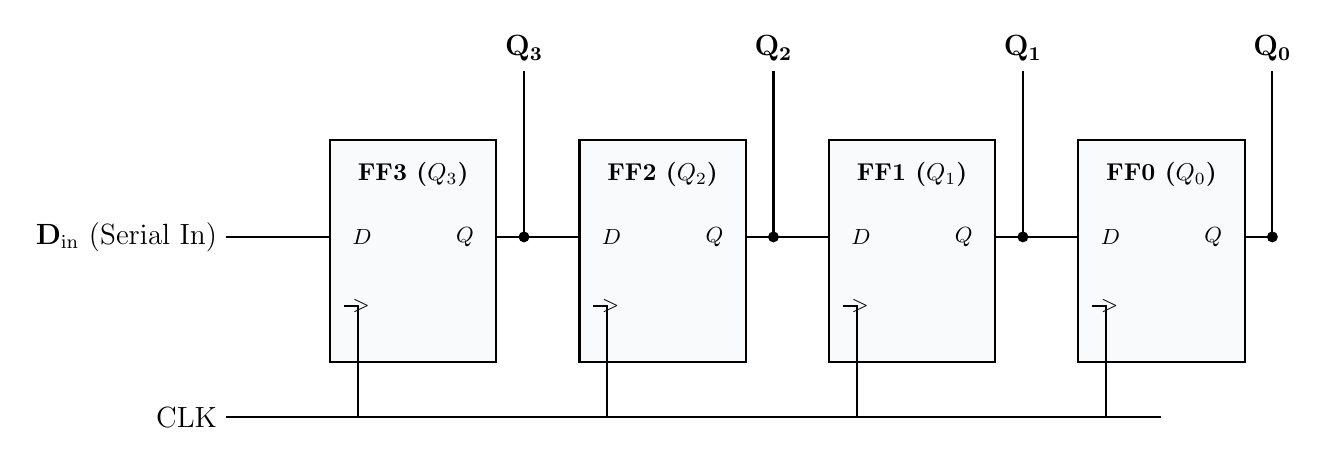
\begin{tikzpicture}[scale=0.88, transform shape]
  % 4 D Flip-Flops
  \foreach \i/\ffname in {3/FF3 ($Q_3$), 2/FF2 ($Q_2$), 1/FF1 ($Q_1$), 0/FF0 ($Q_0$)} {
    \draw[thick, fill=boxbg] ({3.6*(3 - \i)}, 0) rectangle ({3.6*(3 - \i) + 2.4}, 3.2);
    \node at ({3.6*(3 - \i) + 1.2}, 2.7) {\textbf{\ffname}};
    \node[anchor=west] at ({3.6*(3 - \i) + 0.2}, 1.8) {\small $D$};
    \node[anchor=west] at ({3.6*(3 - \i) + 0.2}, 0.8) {\small $>$};
    \node[anchor=east] at ({3.6*(3 - \i) + 2.2}, 1.8) {\small $Q$};
    
    % Parallel output taps
    \filldraw[black] ({3.6*(3 - \i) + 2.8}, 1.8) circle (2pt);
    \draw[thick] ({3.6*(3 - \i) + 2.8}, 1.8) -- ({3.6*(3 - \i) + 2.8}, 4.2) node[above] {\large $\mathbf{Q_\i}$};
  }

  % Serial Input to FF3
  \draw[thick] (-1.5, 1.8) node[left] {\large $\mathbf{D_{\text{in}}\ (\text{Serial In})}$} -- (0, 1.8);

  % Inter-stage connections
  \draw[thick] (2.4, 1.8) -- (3.6, 1.8);
  \draw[thick] (6.0, 1.8) -- (7.2, 1.8);
  \draw[thick] (9.6, 1.8) -- (10.8, 1.8);
  \draw[thick] (13.2, 1.8) -- (13.6, 1.8);

  % Common Clock Rail
  \draw[thick] (-1.5, -0.8) node[left] {\large $\mathbf{\text{CLK}}$} -- (12.0, -0.8);
  \foreach \i in {0,1,2,3} {
    \draw[thick] ({3.6*\i + 0.4}, -0.8) -- ({3.6*\i + 0.4}, 0.8) -- ({3.6*\i + 0.2}, 0.8);
  }
\end{tikzpicture}
\end{schematicbox}

\paragraph{2. Shift Sequence Table for $1011_2$ (MSB entered first):}
Assume initial contents $Q_3 Q_2 Q_1 Q_0 = 0000_2$.
\begin{center}
\begin{tabular}{|c|c|cccc|l|}
\hline
\textbf{Clock Pulse} & \textbf{Serial Input ($D_{\text{in}}$)} & $\mathbf{Q_3}$ & $\mathbf{Q_2}$ & $\mathbf{Q_1}$ & $\mathbf{Q_0}$ & \textbf{State Summary} \\ \hline
\textbf{Initial} & $-$ & 0 & 0 & 0 & 0 & Cleared state \\ \hline
\textbf{CLK 1} & $1$ (MSB) & 1 & 0 & 0 & 0 & First bit into FF3 \\ \hline
\textbf{CLK 2} & $0$ & 0 & 1 & 0 & 0 & Shift right, second bit in \\ \hline
\textbf{CLK 3} & $1$ & 1 & 0 & 1 & 0 & Shift right, third bit in \\ \hline
\textbf{CLK 4} & $1$ (LSB) & 1 & 1 & 0 & 1 & Complete word loaded ($1011_2$) \\ \hline
\end{tabular}
\end{center}

\begin{schematicbox}{Timing Waveforms for Shifting $1011_2$ into SIPO Register}
\centering
\begin{tikzpicture}[scale=0.9, transform shape]
  % Vertical grid lines
  \foreach \x in {0, 2.5, 5.0, 7.5, 10.0, 12.5} {
    \draw[dotted, gray!60] (\x, 1.2) -- (\x, -6.5);
  }
  
  % Clock Waveform
  \node[left] at (-0.3, 0.5) {\textbf{CLK}};
  \draw[thick, blue] (0,0) -- (1.25,0) -- (1.25,1) -- (2.5,1) -- (2.5,0) -- (3.75,0) -- (3.75,1) -- (5.0,1) -- (5.0,0) -- (6.25,0) -- (6.25,1) -- (7.5,1) -- (7.5,0) -- (8.75,0) -- (8.75,1) -- (10.0,1) -- (10.0,0) -- (11.25,0) -- (11.25,1) -- (12.5,1);
  \node at (1.87, 1.3) {\small Pulse 1};
  \node at (4.37, 1.3) {\small Pulse 2};
  \node at (6.87, 1.3) {\small Pulse 3};
  \node at (9.37, 1.3) {\small Pulse 4};

  % Serial In (1, 0, 1, 1)
  \node[left] at (-0.3, -0.8) {\textbf{$D_{\text{in}}$}};
  \draw[thick, red] (0, -0.3) -- (2.5, -0.3) -- (2.5, -1.3) -- (5.0, -1.3) -- (5.0, -0.3) -- (10.0, -0.3) -- (10.0, -1.3) -- (12.5, -1.3);
  \node at (1.25, -0.1) {\small '1'}; \node at (3.75, -1.5) {\small '0'}; \node at (6.25, -0.1) {\small '1'}; \node at (8.75, -0.1) {\small '1'};

  % Q3
  \node[left] at (-0.3, -2.3) {\textbf{$Q_3$}};
  \draw[thick, teal] (0, -2.8) -- (2.5, -2.8) -- (2.5, -1.8) -- (5.0, -1.8) -- (5.0, -2.8) -- (7.5, -2.8) -- (7.5, -1.8) -- (12.5, -1.8);
\end{tikzpicture}
\end{schematicbox}

\begin{answerbox}
Parallel output after 4 clock pulses is $\mathbf{Q_3 Q_2 Q_1 Q_0 = 1101_2}$ (corresponding to serial arrival sequence $1011_2$).
\end{answerbox}

\vspace{0.6cm}

% =========================================================================
% QUESTION 8
% =========================================================================
\subsection{Question 8: 3-Bit Asynchronous UP/DOWN Counter Schematic [5 Marks]}
\begin{questionbox}{Problem Statement (2081 Ashwin, Q8)}
Explain the operation of 3-bit asynchronous up/down counter with logic diagram.
\end{questionbox}

An asynchronous UP/DOWN counter uses a control line $M$ to steer either the normal output $Q$ (for DOWN counting with negative-edge clocking) or inverted output $\bar{Q}$ (for UP counting with negative-edge clocking) to the clock input of the next stage:
\[
\text{CLK}_{i+1} = \bar{M} Q_i + M \bar{Q}_i = M \oplus Q_i
\]

\begin{schematicbox}{3-Bit Negative-Edge Triggered Asynchronous UP/DOWN Counter}
\centering
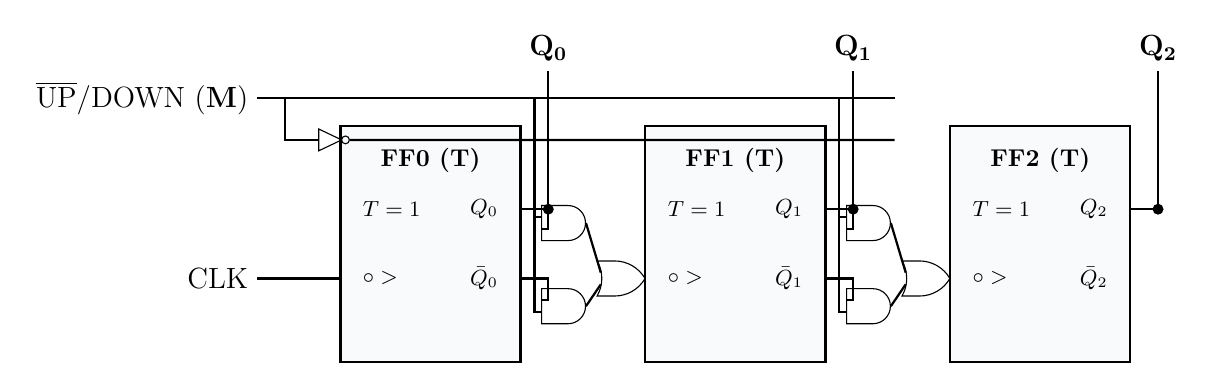
\begin{tikzpicture}[scale=0.88, transform shape]
  % 3 T Flip Flops
  \foreach \i in {0,1,2} {
    \draw[thick, fill=boxbg] ({4.4*\i}, 0) rectangle ({4.4*\i + 2.6}, 3.4);
    \node at ({4.4*\i + 1.3}, 2.9) {\textbf{FF\i\ (T)}};
    \node[anchor=west] at ({4.4*\i + 0.2}, 2.2) {\small $T=1$};
    \node[anchor=west] at ({4.4*\i + 0.2}, 1.2) {\small $\circ>$};
    \node[anchor=east] at ({4.4*\i + 2.4}, 2.2) {\small $Q_\i$};
    \node[anchor=east] at ({4.4*\i + 2.4}, 1.2) {\small $\bar{Q}_\i$};

    \filldraw[black] ({4.4*\i + 3.0}, 2.2) circle (2pt);
    \draw[thick] ({4.4*\i + 2.6}, 2.2) -- ({4.4*\i + 3.0}, 2.2) -- ({4.4*\i + 3.0}, 4.2) node[above] {\large $\mathbf{Q_\i}$};
  }

  % External Clock to FF0
  \draw[thick] (-1.2, 1.2) node[left] {\large $\mathbf{\text{CLK}}$} -- (0, 1.2);

  % Steering Logic between FF0 and FF1
  \node[and gate US, draw, logic gate inputs=nn] (and0a) at (3.2, 2.0) {};
  \node[and gate US, draw, logic gate inputs=nn] (and0b) at (3.2, 0.8) {};
  \node[or gate US, draw, logic gate inputs=nn] (or0) at (4.0, 1.2) {};
  \draw[thick] (2.6, 2.2) -- (3.0, 2.2) |- (and0a.input 2);
  \draw[thick] (2.6, 1.2) -- (3.0, 1.2) |- (and0b.input 1);
  \draw[thick] (and0a.output) -- (or0.input 1);
  \draw[thick] (and0b.output) -- (or0.input 2);
  \draw[thick] (or0.output) -- (4.4, 1.2);

  % Steering Logic between FF1 and FF2
  \node[and gate US, draw, logic gate inputs=nn] (and1a) at (7.6, 2.0) {};
  \node[and gate US, draw, logic gate inputs=nn] (and1b) at (7.6, 0.8) {};
  \node[or gate US, draw, logic gate inputs=nn] (or1) at (8.4, 1.2) {};
  \draw[thick] (7.0, 2.2) -- (7.4, 2.2) |- (and1a.input 2);
  \draw[thick] (7.0, 1.2) -- (7.4, 1.2) |- (and1b.input 1);
  \draw[thick] (and1a.output) -- (or1.input 1);
  \draw[thick] (and1b.output) -- (or1.input 2);
  \draw[thick] (or1.output) -- (8.8, 1.2);

  % Mode Control Rails (UP = M_bar, DOWN = M)
  \draw[thick] (-1.2, 3.8) node[left] {\large $\mathbf{\overline{\text{UP}}/\text{DOWN}\ (M)}$} -- (8.0, 3.8);
  \draw[thick] (2.8, 3.8) |- (and0b.input 2);
  \draw[thick] (7.2, 3.8) |- (and1b.input 2);

  \node[not gate US, draw, scale=0.8] (notM) at (-0.2, 3.2) {};
  \draw[thick] (-0.8, 3.8) |- (notM.input);
  \draw[thick] (notM.output) -- (8.0, 3.2);
  \draw[thick] (2.8, 3.2) |- (and0a.input 1);
  \draw[thick] (7.2, 3.2) |- (and1a.input 1);
\end{tikzpicture}
\end{schematicbox}

\begin{answerbox}
$$\mathbf{M=0 \implies \text{UP Counting } (Q_0 \to \text{CLK}_1, Q_1 \to \text{CLK}_2), \qquad M=1 \implies \text{DOWN Counting } (\bar{Q}_0 \to \text{CLK}_1, \bar{Q}_1 \to \text{CLK}_2)}$$
\end{answerbox}

\vspace{0.6cm}

% =========================================================================
% QUESTION 9
% =========================================================================
\subsection{Question 9: Synchronous FSM Sequence Detector '101' [7 Marks]}
\begin{questionbox}{Problem Statement (2081 Ashwin, Q9)}
Design a synchronous sequential machine that has 1-bit serial input $X$ and output $Z$ which will be high when the input contains the message `101' (Use SR Flip-Flop).
\end{questionbox}

\paragraph{1. State Definitions and State Transition Diagram (Mealy Model):}
\begin{itemize}
  \item $S_0 (00)$: Reset state.
  \item $S_1 (01)$: Sequence `1' detected.
  \item $S_2 (10)$: Sequence `10' detected.
  \item In $S_2$, when $X=1 \implies$ `101' detected $\implies Z=1$, next state $S_1$ (overlapping allowed).
\end{itemize}

\begin{schematicbox}{State Transition Diagram for '101' Sequence Detector}
\centering
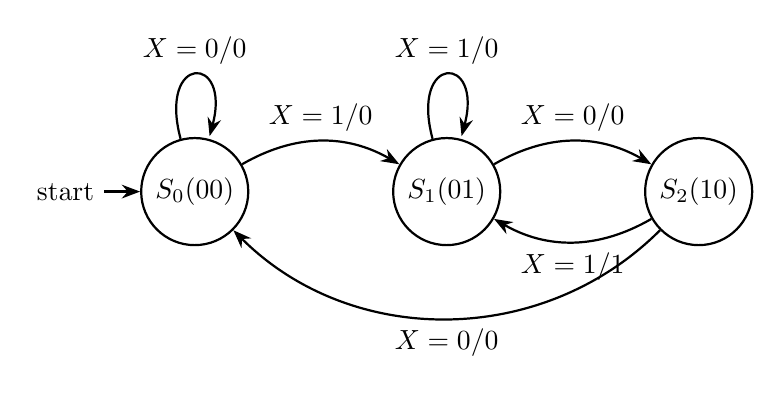
\begin{tikzpicture}[->, >=Stealth, auto, node distance=3.2cm, thick]
  \node[state, initial] (S0) {$S_0 (00)$};
  \node[state] (S1) [right of=S0] {$S_1 (01)$};
  \node[state] (S2) [right of=S1] {$S_2 (10)$};

  \path (S0) edge [loop above] node {$X=0 / 0$} (S0)
             edge [bend left] node {$X=1 / 0$} (S1)
        (S1) edge [loop above] node {$X=1 / 0$} (S1)
             edge [bend left] node {$X=0 / 0$} (S2)
        (S2) edge [bend left] node {$X=1 / 1$} (S1)
             edge [bend left=45] node {$X=0 / 0$} (S0);
\end{tikzpicture}
\end{schematicbox}

\paragraph{2. State and Excitation Table for SR Flip-Flops ($A, B$):}
\begin{center}
\begin{tabular}{|cc|c|cc|c|cccc|}
\hline
\multicolumn{2}{|c|}{\textbf{Present State}} & \textbf{Input} & \multicolumn{2}{c|}{\textbf{Next State}} & \textbf{Output} & \multicolumn{4}{c|}{\textbf{SR Inputs}} \\
$A$ & $B$ & $X$ & $A^+$ & $B^+$ & $\mathbf{Z}$ & $\mathbf{S_A}$ & $\mathbf{R_A}$ & $\mathbf{S_B}$ & $\mathbf{R_B}$ \\ \hline
0 & 0 & 0 & 0 & 0 & 0 & 0 & $X$ & 0 & $X$ \\ \hline
0 & 0 & 1 & 0 & 1 & 0 & 0 & $X$ & 1 & 0 \\ \hline
0 & 1 & 0 & 1 & 0 & 0 & 1 & 0 & 0 & 1 \\ \hline
0 & 1 & 1 & 0 & 1 & 0 & 0 & $X$ & $X$ & 0 \\ \hline
1 & 0 & 0 & 0 & 0 & 0 & 0 & 1 & 0 & $X$ \\ \hline
1 & 0 & 1 & 0 & 1 & 1 & 0 & 1 & 1 & 0 \\ \hline
1 & 1 & 0 & $X$ & $X$ & $X$ & $X$ & $X$ & $X$ & $X$ \\ \hline
1 & 1 & 1 & $X$ & $X$ & $X$ & $X$ & $X$ & $X$ & $X$ \\ \hline
\end{tabular}
\end{center}

\paragraph{3. Minimized Equations via K-Maps:}
\begin{align*}
S_A &= B\bar{X} \\
R_A &= X + \bar{B} \\
S_B &= \bar{A}X \\
R_B &= \bar{X} \\
Z &= AX
\end{align*}

\begin{schematicbox}{Complete Synchronous Logic Schematic Using SR Flip-Flops}
\centering
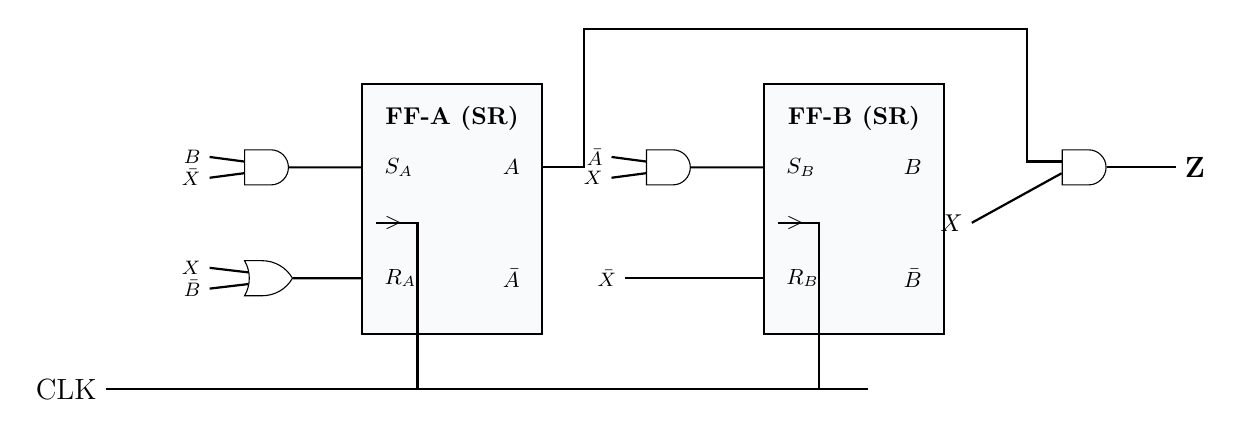
\begin{tikzpicture}[scale=0.88, transform shape]
  % 2 SR Flip Flops
  \draw[thick, fill=boxbg] (2.2, 0) rectangle (4.8, 3.6);
  \node at (3.5, 3.1) {\textbf{FF-A (SR)}};
  \node[anchor=west] at (2.4, 2.4) {\small $S_A$};
  \node[anchor=west] at (2.4, 1.6) {\small $>$};
  \node[anchor=west] at (2.4, 0.8) {\small $R_A$};
  \node[anchor=east] at (4.6, 2.4) {\small $A$};
  \node[anchor=east] at (4.6, 0.8) {\small $\bar{A}$};

  \draw[thick, fill=boxbg] (8.0, 0) rectangle (10.6, 3.6);
  \node at (9.3, 3.1) {\textbf{FF-B (SR)}};
  \node[anchor=west] at (8.2, 2.4) {\small $S_B$};
  \node[anchor=west] at (8.2, 1.6) {\small $>$};
  \node[anchor=west] at (8.2, 0.8) {\small $R_B$};
  \node[anchor=east] at (10.4, 2.4) {\small $B$};
  \node[anchor=east] at (10.4, 0.8) {\small $\bar{B}$};

  % Clock
  \draw[thick] (-1.5, -0.8) node[left] {\large $\mathbf{\text{CLK}}$} -- (9.5, -0.8);
  \draw[thick] (3.0, -0.8) -- (3.0, 1.6) -- (2.4, 1.6);
  \draw[thick] (8.8, -0.8) -- (8.8, 1.6) -- (8.2, 1.6);

  % Combinational Gates for FF-A:
  % S_A = B . X_bar
  \node[and gate US, draw, logic gate inputs=nn] (andSA) at (0.8, 2.4) {};
  \draw[thick] (0, 2.55) node[left] {\footnotesize $B$} -- (andSA.input 1);
  \draw[thick] (0, 2.25) node[left] {\footnotesize $\bar{X}$} -- (andSA.input 2);
  \draw[thick] (andSA.output) -- (2.2, 2.4);

  % R_A = X + B_bar
  \node[or gate US, draw, logic gate inputs=nn] (orRA) at (0.8, 0.8) {};
  \draw[thick] (0, 0.95) node[left] {\footnotesize $X$} -- (orRA.input 1);
  \draw[thick] (0, 0.65) node[left] {\footnotesize $\bar{B}$} -- (orRA.input 2);
  \draw[thick] (orRA.output) -- (2.2, 0.8);

  % Combinational Gates for FF-B:
  % S_B = A_bar . X
  \node[and gate US, draw, logic gate inputs=nn] (andSB) at (6.6, 2.4) {};
  \draw[thick] (5.8, 2.55) node[left] {\footnotesize $\bar{A}$} -- (andSB.input 1);
  \draw[thick] (5.8, 2.25) node[left] {\footnotesize $X$} -- (andSB.input 2);
  \draw[thick] (andSB.output) -- (8.0, 2.4);

  % R_B = X_bar
  \draw[thick] (6.0, 0.8) node[left] {\footnotesize $\bar{X}$} -- (8.0, 0.8);

  % Output Z = A . X
  \node[and gate US, draw, logic gate inputs=nn] (andZ) at (12.6, 2.4) {};
  \draw[thick] (4.8, 2.4) -- (5.4, 2.4) -- (5.4, 4.4) -- (11.8, 4.4) |- (andZ.input 1);
  \draw[thick] (11.0, 1.6) node[left] {$X$} -- (andZ.input 2);
  \draw[thick] (andZ.output) -- ++(1.0, 0) node[right] {\large $\mathbf{Z}$};
\end{tikzpicture}
\end{schematicbox}

\begin{answerbox}
$$\mathbf{S_A = B\bar{X}, \quad R_A = X + \bar{B}, \quad S_B = \bar{A}X, \quad R_B = \bar{X}, \quad Z = AX}$$
\end{answerbox}

\vspace{0.6cm}

% =========================================================================
% QUESTION 9
% =========================================================================
\subsection{Question 9: Two-Input TTL NOR Gate Transistor Circuit [5 + 2 = 7 Marks]}
\begin{questionbox}{Problem Statement (2081 Ashwin, Q9)}
Draw the circuit diagram of two-input TTL NOR gate and explain its logic operation briefly and list the characteristics of CMOS logic family.
\end{questionbox}

\paragraph{Part (a): 2-Input TTL NOR Gate Transistor Circuit \& Operation [5 Marks]}
A Transistor-Transistor Logic (TTL) NOR gate uses:
\begin{itemize}
  \item \textbf{Dual Input Stages (Parallel branches):}
  \begin{itemize}
    \item Input $A$ drives input transistor $Q_1$ (with pull-up $R_1 = 4\text{k}\Omega$) which controls phase-splitter $Q_3$.
    \item Input $B$ drives input transistor $Q_2$ (with pull-up $R_2 = 4\text{k}\Omega$) which controls phase-splitter $Q_4$.
  \end{itemize}
  \item \textbf{Parallel Phase Splitters ($Q_3 \parallel Q_4$):}
  $Q_3$ and $Q_4$ share a common collector load ($R_3 = 1.6\text{k}\Omega$) and a common emitter resistor ($R_4 = 1\text{k}\Omega$).
  \item \textbf{Output Totem-Pole Stage:}
  Upper active pull-up transistor $Q_5$ with series diode $D_1$ and current-limiting resistor $R_5 = 130\Omega$, and lower pull-down transistor $Q_6$.
\end{itemize}

\begin{schematicbox}{Transistor Schematic of 2-Input Standard TTL NOR Gate}
\centering
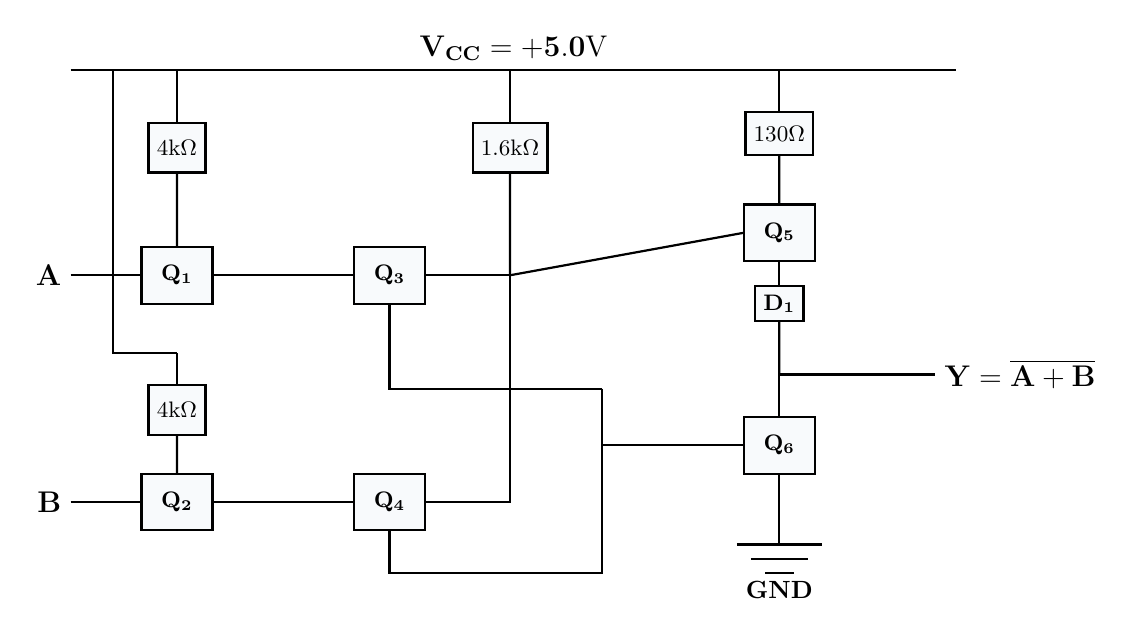
\begin{tikzpicture}[scale=0.9, transform shape]
  % VCC Rail
  \draw[thick] (0, 7.5) -- (12.5, 7.5);
  \node[above] at (6.25, 7.5) {\large $\mathbf{V_{CC} = +5.0\text{V}}$};

  % TOP BRANCH: Input A -> Q1 -> Q3
  % R1
  \draw[thick] (1.5, 7.5) -- (1.5, 6.4) node[draw, fill=boxbg, minimum width=0.6cm, minimum height=0.7cm] (r1) {\small $4\text{k}\Omega$};
  \draw[thick] (r1.south) -- (1.5, 5.0);
  % Q1
  \draw[thick, fill=boxbg] (1.0, 4.2) rectangle (2.0, 5.0); \node at (1.5, 4.6) {\small $\mathbf{Q_1}$};
  \draw[thick] (0.0, 4.6) node[left] {\large $\mathbf{A}$} -- (1.0, 4.6);
  % Q3
  \draw[thick, fill=boxbg] (4.0, 4.2) rectangle (5.0, 5.0); \node at (4.5, 4.6) {\small $\mathbf{Q_3}$};
  \draw[thick] (2.0, 4.6) -- (4.0, 4.6); % Q1 coll to Q3 base

  % BOTTOM BRANCH: Input B -> Q2 -> Q4
  % R2
  \draw[thick] (1.5, 3.5) -- (1.5, 2.7) node[draw, fill=boxbg, minimum width=0.6cm, minimum height=0.7cm] (r2) {\small $4\text{k}\Omega$};
  \draw[thick] (1.5, 7.5) -| (0.6, 3.5) -- (1.5, 3.5);
  \draw[thick] (r2.south) -- (1.5, 1.8);
  % Q2
  \draw[thick, fill=boxbg] (1.0, 1.0) rectangle (2.0, 1.8); \node at (1.5, 1.4) {\small $\mathbf{Q_2}$};
  \draw[thick] (0.0, 1.4) node[left] {\large $\mathbf{B}$} -- (1.0, 1.4);
  % Q4
  \draw[thick, fill=boxbg] (4.0, 1.0) rectangle (5.0, 1.8); \node at (4.5, 1.4) {\small $\mathbf{Q_4}$};
  \draw[thick] (2.0, 1.4) -- (4.0, 1.4); % Q2 coll to Q4 base

  % Common Phase Splitter Collector Load R3
  \draw[thick] (6.2, 7.5) -- (6.2, 6.4) node[draw, fill=boxbg, minimum width=0.6cm, minimum height=0.7cm] (r3) {\small $1.6\text{k}\Omega$};
  \draw[thick] (r3.south) -- (6.2, 4.6);
  \draw[thick] (5.0, 4.6) -- (6.2, 4.6);
  \draw[thick] (5.0, 1.4) -- (6.2, 1.4) -- (6.2, 4.6);

  % Common Phase Splitter Emitter to Q6 Base and R4
  \draw[thick] (4.5, 4.2) -- (4.5, 3.0) -- (7.5, 3.0);
  \draw[thick] (4.5, 1.0) -- (4.5, 0.4) -- (7.5, 0.4) |- (7.5, 3.0);

  % Totem Pole Stage: Q5, D1, Q6
  % R5
  \draw[thick] (10.0, 7.5) -- (10.0, 6.6) node[draw, fill=boxbg, minimum width=0.6cm, minimum height=0.6cm] (r5) {\small $130\Omega$};
  \draw[thick] (r5.south) -- (10.0, 5.6);
  % Q5
  \draw[thick, fill=boxbg] (9.5, 4.8) rectangle (10.5, 5.6); \node at (10.0, 5.2) {\small $\mathbf{Q_5}$};
  \draw[thick] (6.2, 4.6) -- (9.5, 5.2); % Base of Q5

  % D1
  \draw[thick] (10.0, 4.8) -- (10.0, 4.2) node[draw, fill=boxbg, minimum width=0.6cm, minimum height=0.4cm] (d1) {\small $\mathbf{D_1}$};
  \draw[thick] (d1.south) -- (10.0, 3.2);

  % Q6
  \draw[thick, fill=boxbg] (9.5, 1.8) rectangle (10.5, 2.6); \node at (10.0, 2.2) {\small $\mathbf{Q_6}$};
  \draw[thick] (7.5, 3.0) |- (9.5, 2.2); % Base of Q6 from phase splitters
  \draw[thick] (10.0, 3.2) -- (10.0, 2.6);

  % Output node Y
  \draw[thick] (10.0, 3.2) -- (12.2, 3.2) node[right] {\large $\mathbf{Y = \overline{A + B}}$};

  % Ground
  \draw[thick] (10.0, 1.8) -- (10.0, 0.8);
  \draw[thick] (9.4, 0.8) -- (10.6, 0.8);
  \draw[thick] (9.6, 0.6) -- (10.4, 0.6);
  \draw[thick] (9.8, 0.4) -- (10.2, 0.4);
  \node[below] at (10.0, 0.4) {\textbf{GND}};
\end{tikzpicture}
\end{schematicbox}

\paragraph{Logic Operation Table:}
\begin{center}
\begin{tabular}{|cc||cc|cc|cc||c|l|}
\hline
$\mathbf{A}$ & $\mathbf{B}$ & $\mathbf{Q_1}$ & $\mathbf{Q_2}$ & $\mathbf{Q_3}$ & $\mathbf{Q_4}$ & $\mathbf{Q_5}$ & $\mathbf{Q_6}$ & $\mathbf{Y}$ & \textbf{Logic State} \\ \hline
0 & 0 & Sat & Sat & OFF & OFF & ON & OFF & $\mathbf{1}\ (\approx 3.4\text{V})$ & High Output ($V_{OH}$) \\ \hline
0 & 1 & Sat & Inv & OFF & ON & OFF & ON & $\mathbf{0}\ (\approx 0.2\text{V})$ & Low Output ($V_{OL}$) \\ \hline
1 & 0 & Inv & Sat & ON & OFF & OFF & ON & $\mathbf{0}\ (\approx 0.2\text{V})$ & Low Output ($V_{OL}$) \\ \hline
1 & 1 & Inv & Inv & ON & ON & OFF & ON & $\mathbf{0}\ (\approx 0.2\text{V})$ & Low Output ($V_{OL}$) \\ \hline
\end{tabular}
\end{center}

\paragraph{Part (b): Characteristics of CMOS Logic Family [2 Marks]}
\begin{enumerate}
  \item \textbf{Extremely Low Static Power Consumption:} Near zero ($< 10\text{ nW}$ per gate), power is consumed only during switching transitions.
  \item \textbf{Wide Supply Voltage Range:} Operates reliably from $+3\text{V}$ to $+15\text{V}$ (4000 series) or $+2\text{V}$ to $+6\text{V}$ (74HC series).
  \item \textbf{Very High Noise Immunity:} Noise margin is typically $40\%$ to $45\%$ of $V_{DD}$ ($> 1.5\text{V}$ at $V_{DD}=5\text{V}$).
  \item \textbf{Extremely High Fan-Out:} Fan-out $> 50$ due to nearly infinite MOSFET input resistance ($R_{\text{in}} > 10^{12}\ \Omega$).
  \item \textbf{Full Rail-to-Rail Output Swing:} $V_{OH} \approx V_{DD}$ and $V_{OL} \approx 0\text{V}$.
\end{enumerate}

\begin{answerbox}
The TTL NOR gate uses parallel phase splitters ($Q_3, Q_4$) to pull the totem-pole output LOW whenever either input is HIGH. CMOS logic provides near-zero static power dissipation and high noise margins.
\end{answerbox}

\vspace{0.6cm}

% =========================================================================
% QUESTION 10
% =========================================================================
\subsection{Question 10: Digital Frequency Measurement Block Diagram [4 Marks]}
\begin{questionbox}{Problem Statement (2081 Ashwin, Q10)}
With the help of functional diagram explain the operation of frequency measurement.
\end{questionbox}

A \textbf{Digital Frequency Measurement System} determines the unknown frequency $f_x$ of an input waveform by accumulating the count of input cycles during a calibrated time gate interval $T_{\text{gate}}$:
\[
f_x = \frac{N}{T_{\text{gate}}}
\]

\paragraph{Operational Principle:}
\begin{enumerate}
  \item \textbf{Input Waveform Conditioning:} The unknown periodic analog signal is amplified and passed through a \textbf{Schmitt Trigger}, converting it into a clean train of digital clock pulses of frequency $f_x$.
  \item \textbf{Time Base Generation:} A high-precision crystal oscillator (e.g. 1 MHz, stability $\pm 1\text{ ppm}$) feeds a chain of decade frequency dividers to synthesize accurate gate open times $T_{\text{gate}} = 1\text{ s}, 0.1\text{ s}, 10\text{ ms}$.
  \item \textbf{Gating Logic:} The Main AND Gate is enabled by the gate control bistable multivibrator for exactly $T_{\text{gate}}$. Exactly $N = f_x \times T_{\text{gate}}$ pulses pass through the gate.
  \item \textbf{Decade Counting \& Readout:} The cascaded BCD counter counts $N$ pulses, transfers the result to a latch register, and illuminates the 7-segment digital display.
\end{enumerate}

\begin{schematicbox}{Block Diagram of Digital Frequency Measurement System}
\centering
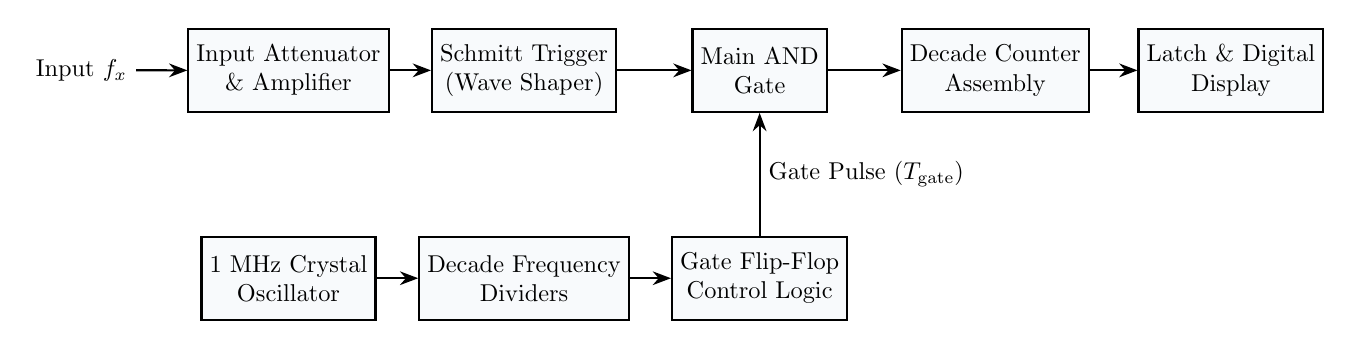
\begin{tikzpicture}[scale=0.88, transform shape, >=Stealth]
  % Input channel
  \node[draw, thick, fill=boxbg, minimum width=2.2cm, minimum height=1.2cm, align=center] (amp) at (0, 3) {Input Attenuator\\\& Amplifier};
  \node[draw, thick, fill=boxbg, minimum width=2.2cm, minimum height=1.2cm, align=center] (schmitt) at (3.4, 3) {Schmitt Trigger\\(Wave Shaper)};
  \node[draw, thick, fill=boxbg, minimum width=1.8cm, minimum height=1.2cm, align=center] (gate) at (6.8, 3) {Main AND\\Gate};
  \node[draw, thick, fill=boxbg, minimum width=2.4cm, minimum height=1.2cm, align=center] (count) at (10.2, 3) {Decade Counter\\Assembly};
  \node[draw, thick, fill=boxbg, minimum width=2.2cm, minimum height=1.2cm, align=center] (disp) at (13.6, 3) {Latch \& Digital\\Display};

  \draw[thick, ->] (-2.2, 3) node[left] {Input $f_x$} -- (amp.west);
  \draw[thick, ->] (amp.east) -- (schmitt.west);
  \draw[thick, ->] (schmitt.east) -- (gate.west);
  \draw[thick, ->] (gate.east) -- (count.west);
  \draw[thick, ->] (count.east) -- (disp.west);

  % Time Base channel
  \node[draw, thick, fill=boxbg, minimum width=2.2cm, minimum height=1.2cm, align=center] (osc) at (0, 0) {1 MHz Crystal\\Oscillator};
  \node[draw, thick, fill=boxbg, minimum width=2.4cm, minimum height=1.2cm, align=center] (div) at (3.4, 0) {Decade Frequency\\Dividers};
  \node[draw, thick, fill=boxbg, minimum width=2.2cm, minimum height=1.2cm, align=center] (ctrl) at (6.8, 0) {Gate Flip-Flop\\Control Logic};

  \draw[thick, ->] (osc.east) -- (div.west);
  \draw[thick, ->] (div.east) -- (ctrl.west);
  \draw[thick, ->] (ctrl.north) -- (gate.south) node[midway, right] {Gate Pulse ($T_{\text{gate}}$)};
\end{tikzpicture}
\end{schematicbox}

\begin{answerbox}
Frequency is measured by counting $N$ conditioned input pulses over a precision gate window $T_{\text{gate}}$ via the formula $\mathbf{f_x = N / T_{\text{gate}}}$.
\end{answerbox}

\end{document}
